\documentclass[11pt, oneside]{report}   	% use "amsart" instead of "article" for AMSLaTeX format
\usepackage[margin = 1in]{geometry}                		% See geometry.pdf to learn the layout options. There are lots.
\geometry{a4paper}                   		% ... or a4paper or a5paper or ... 
%\geometry{landscape}                		% Activate for rotated page geometry
\usepackage[parfill]{parskip}    		% Activate to begin paragraphs with an empty line rather than an indent
\usepackage{graphicx}				% Use pdf, png, jpg, or eps§ with pdflatex; use eps in DVI mode
								% TeX will automatically convert eps --> pdf in pdflatex	
\usepackage{subcaption}									
\usepackage{amsfonts, amsmath,amssymb}
\usepackage{siunitx}
\usepackage[none]{hyphenat}
\usepackage{fancyhdr}
\usepackage{setspace}
\usepackage{hyperref}
%\usepackage[nottoc, notlot, notlof]{tocbibind}		%table of contents
\usepackage{helvet}
\renewcommand{\familydefault}{\sfdefault}

\usepackage{wrapfig}

\usepackage{multirow}
\usepackage[table,xcdraw]{xcolor}
\usepackage{array}
\newcolumntype{L}{>{\centering\arraybackslash}m{6.5cm}}

\usepackage{csquotes}

\usepackage{epstopdf}
\DeclareGraphicsExtensions{.pdf,.png,.jpg,.eps}

\usepackage{titlesec}
%\titlespacing\chapter{0pt}{4pt plus 4pt minus 2pt}{4pt plus 2pt minus 2pt}
\titlespacing\section{0pt}{4pt plus 4pt minus 2pt}{0pt plus 2pt minus 2pt}
\titlespacing\subsection{0pt}{4pt plus 4pt minus 2pt}{0pt plus 2pt minus 2pt}
\titlespacing\subsubsection{0pt}{4pt plus 4pt minus 2pt}{0pt plus 2pt minus 2pt}

\AtBeginDocument{%
	\abovedisplayskip=3pt plus 3pt minus 3pt
	\abovedisplayshortskip=0pt plus 3pt
	\belowdisplayskip=3pt plus 3pt minus 3pt
	\belowdisplayshortskip=7pt plus 3pt minus 4pt
}

\titleformat{\chapter}[display]
{\normalfont\huge\bfseries}{\chaptertitlename\ \thechapter}{0pt}{\Huge}
\titlespacing*{\chapter}{0pt}{0pt}{0pt}

\usepackage{sidecap}

\pagestyle{fancy}
\fancyhead{}
\fancyfoot{}
\fancyhead[L]{\slshape \MakeUppercase{4YP Report}}
\fancyhead[R]{\slshape 355136}
\fancyfoot[C]{\thepage}
%\renewcommand{\headrulewidth}{0pt} %remove line in header

\setlength{\parskip}{1em}
\doublespacing

% alternative margin for declaration page
\newenvironment{changemargin}[3]{%
\begin{list}{}{%
\setlength{\topsep}{0pt}%
\setlength{\leftmargin}{#1}%
\setlength{\rightmargin}{#2}%
\setlength{\topmargin}{#3}%
\setlength{\listparindent}{\parindent}%
\setlength{\itemindent}{\parindent}%
\setlength{\parsep}{\parskip}%
}%
\item[]}{\end{list}}


\usepackage{mathtools}
\newcommand\SmallMatrix[1]{{%
  \big\arraycolsep=0.5\arraycolsep\ensuremath{\begin{pmatrix}#1\end{pmatrix}}}}
\DeclareMathOperator{\diag}{diag}
%\DeclareMathOperator{\f}{f}

\renewcommand{\vec}[1]{\mathbf{#1}}


\title{B1 Project Report}
\author{Candidate Number: 355136}
\date{}							% Activate to display a given date or no date

\begin{document}
\pagenumbering{Roman}

\begin{titlepage}
\begin{center}
\vspace*{1cm}
\Large {\textbf{The University of Oxford}}\\
\Large{\textbf{Engineering Science}}\\
\vfill
\noindent\rule{5in}{0.6pt}\\[1mm]
\huge{\textbf{4YP Project Report}}\\[3mm]
\Large{\textbf{- Using Machine Learning to Control Software Synthesisers  -}}\\[1mm]
\noindent\rule{5in}{0.6pt}\\[1mm]
\vfill
Candidate Number: 355136\\
\today\\
\end{center}
\end{titlepage}

%\newgeometry{left=0cm,right=0cm,top=0cm,bottom=0cm}
\begin{changemargin}{-1in}{0in}{-1.5in}

\includegraphics{Declaration_of_Authorship_form_2018.pdf}
\thispagestyle{empty}
\end{changemargin}

\begin{abstract}
\begin{flushleft}
\emph{Software synthesisers} (soft-synths) are computer applications that create sounds in response to musical input, typically in the form of \emph{MIDI} (\emph{Musical Instrument Digital Interface}) messages, and are widely used in a variety of musical contexts. Typical soft-synths have hundreds or thousands of parameters that control the sound generation algorithm, allowing the user to create sounds that suit their musical needs. This results in a high dimensional, non-linear search space that the user must navigate. Research indicates that users struggle to navigate such spaces with serial controls, and that there is a strong link between interface design and the level of creativity that the users experience. \\
This work describes a novel interface designed to help users control synthesisers in a quicker and more intuitive manner. It combines three interfaces together: a traditional `knob and slider' interface, a search space visualisation interface, and an iterative blending interface.\\
%
Suitable types of synthesiser for this interface are identified, and a purpose-built synthesiser created with a small dataset of presets.\\
Principal Component Analysis (PCA) combined with Histogram Equalisation is shown to be an effective method to create a low dimensional embedding of a synthesiser preset dataset.
An algorithm is developed to eliminate an undesirable phenomenon of PCA, in which the sign of the principal components may flip unexpectedly as more data points are added to the dataset.
An algorithm for iteratively generating new presets based off users' preferences is developed.
 A Perfect/Imperfect user model is developed to numerically evaluate syntheiser interfaces.
 Parameter selection order is identified as a key limitation of traditional interfaces.
 To verify the design of the novel interface, it is also tested in a different context - Image Filtering.

\end{flushleft}
\end{abstract}


%\newgeometry{left=1in,right=1in,top=1in,bottom=1in}
\tableofcontents
%\thispagestyle{empty}
\clearpage
\pagenumbering{arabic}
\setcounter{page}{1}


%%%%%%%%%%%%%%%%%%%%%%%%%%%%%%%%%%%%%%%%%%%%%%%%%%%%%%%%%%%%%%%%%%%%%%%%%%%%%

%
%\chapter{Introduction}
%%\section{Background Information}
%Software Synthesisers (Soft-Synths) are computer applications which create sounds in response to musical input typically in the form of \emph{MIDI} (\emph{Musical Instrument Digital Interface}) messages. They are widely used in a variety of musical contexts. Typical soft-synths have hundreds or thousands of parameters which control the sound generation algorithm, allowing the user to create sounds that suit their musical needs. This results in a high dimensional, non-linear search space which the user must navigate. The act of choosing the parameter values for a synth is commonly refered to as \emph{programming} the synth. Research indicates that humans are bad at navigating such interfaces with serial controls \cite{YeeKing}, and that there is a strong link between interface design and the level of creativity that the user with experience when using the interface \cite{TubbThesis}. \\
%This work describes a novel interface designed to help users control synthesisers in a quicker and more intuitive manner. It combines three interfaces together: a traditional 'knob and slider' interface, a search space visualisation interface, and an iterative blending interface.
%
%
%\section{Aims of the project}
%\begin{itemize}
%	\item Create a synthesiser to test the interface with.
%	\item Create dataset of synthesiser presets
%	\item Create low dimensional embedding of the preset dataset
%	\item Prototype the user interface (UI).
%	\item Determine an optimal way to generate new presets for each iteration of the Blending Interface
%	\item Compare the novel interface to a 'traditional' synth interface.
%\end{itemize}
%NEEDS WORK - MAYBE DELETE THE AIMS SECTION AND REPLACE WITH CONTRIBUTIONS, AND REPORT STRUCTURE SECTIONS.
%\section{Methodology}
%The main methodology taken in this project is that the set of preset sounds for a synthesiser contain a lot of useable information. This is because much of the parameter space of typical synthesisers creates inaudible, or terrible sounding sounds, and the presets have been designed to avoid such regions, and to highlight a diverse range of the synth's best sounds. By working to map the timbre of the presets, rather than the timbre of the entire parameter space, a much simpler, and hopefully more useful latent space can be identified, only requiring simpler statistical techniques to be used.
%
%This project aims to make use of human users' impressive abilities of spatial memory, spatial reasoning, and memory of colours to increase the effectiveness of the interface. In particular, effort will be taken to maintain visual consistency between interfaces. (REFERENCE)
%
%Studies show (REFERENCE), that users are much better at giving a preferance between several options, rather that scoring indivudual options numerically. This will be exploited in the Blending Interface, where in each iteration the user selectes between a range of sounds, which were generated based on their previous preferences. (TRY TO DESCRIBE BETTER)
%
%*---- Move to Synth justification Bit?
%The project is aimed at fixed architechure parametric synhesisers, such as FM, additive, subractive, and physical modelling synthesisers. These have a fixed number of parameters which entirely decribe the sound, making parameter-based comparisons between presets possible. 
%NEEDS MORE WORK.
%
%Mention how this work aims to create a fairly lightweight interface, due to resourse contraints of users. Also mention how typical musical interface users will use interfaces in unexpected ways, so its good to keep flexibility in the interface, and allow many different workflows.
%-----*
%
%Mention how in normal synths, the knobs are mapped such that their motion has a (relatively) linear motion though perceptual space, I.e frequency usually as exponential mapping, and time has a Log(?) mapping.


\chapter{Introduction}
The invention and subsequent development of the \emph{synthesiser} (synth) has been one of the main driving forces behind the evolution of popular and experimental music over the last century. With the current ubiquity of cheap, powerful computers, the barriers of entry to music making are lower than ever: award winning albums have been produced by teenagers, entirely on laptops and smartphones \cite{IphoneProducer}. Such productions commonly use \emph{software synthesisers} (soft synths) to produce many of the sounds.\\
Typical soft-synths require considerable technical knowledge to use, and have hundreds or even thousands of \emph{parameters} that control the sound generation algorithm. Many musicians lack the expertise required to synthesise sounds from scratch and thus rely heavily on \emph{presets}, pre-made combinations of parameters which produce useful sounds. Whilst there is nothing necessarily wrong with using presets, it makes it difficult for musicians to create unique and destinctive sounds. There is even a sizeable market for buying new presets for synths.\\
A conclusion can be drawn from this: more work needs to be done to make synths easier to use. To quote Roger Linn, a pioneer of musical interface design, in a 2016 keynote: \cite{LinnKeynote}
\begin{displayquote}
	\singlespacing
	``In the early days of automobiles, to own one you had to know the technical details of how it worked, and clubs of enthusiasts were formed around details such as carburettors and spark plugs. Once cars got more reliable these clubs disappeared, as it turned out they were actually just intersted in the ability to drive. I think this is the area we're in now [with synthesisers]. People are learning every little detail rather than focusing on making music \dots The key challenge of synth design is to find what the musician really wants, and give them controls in that space.''
\end{displayquote}
This project aims to tackle this problem by designing a radically new interface for controlling synths, and along the way hopes to find some useful insights about high-dimensional parameter spaces in general.
%
\section{Key Ideas}
Presets are widely used and very useful to musicians, and so should form a key part of the interface. Furthermore, the presets of a synth contain a lot of useable information. This is because the presets have been designed to highlight a diverse range of the synth's best sounds, avoiding the numerous regions of parameter space which create inaudible, or terrible sounds. By analysing the timbre of the presets, rather than the timbre of the entire parameter space, a simpler, and more useful control space can be identified, whilst only requiring simple statistical techniques to be used.\\
%
Humans have impressive abilities of spatial memory, spatial reasoning, and memory of colours, and this can be exploited to increase the effectiveness of the interface. In particular, effort will be taken to maintain visual consistency between throughout the interface.\\
%
Studies show \cite{RatingRanking, PreferenceGallery}, that users are much better at giving a preferance between several options, rather that scoring individual options numerically. This is exploited in the Blending Interface, where in each iteration the user selects between a range of sounds, which were generated based on their previous preferences.
%
\section{Contributions}
\begin{itemize}
	\setlength\itemsep{-1.0em}
	\item A novel interface is designed, combining a traditional synth interface with a search space visualisation interface, and an iterative blending interface.
	\item Suitable types of synth for this interface are identified, and a purpose built synth created to test the interface with.
	\item A small dataset of synth presets is created
	\item Principal Component Analysis (PCA) combined with Histogram Equalisation is shown to be an effective method to create a low dimensional embedding of a synth preset dataset.
	\item An algorithm is developed to eliminate an undesirable phenomenon of PCA, in which the sign of the principal components may flip unexpectedly as more data points are added.
	\item An algorithm for iteratively generating new presets based off users' preferences is developed.
	\item A Perfect/Imperfect user model is developed to numerically evaluate synth interfaces.
	\item Parameter selection order is identified as a key limitation of traditional interfaces.
	\item To verify the approach, the interface is tested in a different context - Image Filtering.
\end{itemize}


\chapter{Literature Review}
\section{Introduction to Synthesisers}
\emph{Synthesisers} (synths) are devices which can create a wide variety of musical sounds in response to  user input, typically in the form of notes played on a keyboard. The history of synths closely follows the evolution of electronics over the last century.\\
Early synths, 1900 - 1960, used the technologies of the time to create sound. These included steam powered electromagnetic generators, vaccum tubes, electrostatic antennae, and a variety of electro-mechanical technologies \cite{AppleSynth}.\\
In the 1960s and 70s technology from early analogue computers and laboratory test equipment was used to create sound. The invention of the transistor made many types of electronic circuit cheap and practical to use, allowing the creation of  \emph{modular synthesisers}. These consisted of many modules of electronics, such as voltage-controlled oscillators, filters and amplifiers (VCOs, VCFs and VCAs) and envelope generators, which were patched together with cables (Fig. \ref{fig:MoogSystem35}). As this technology matured, many more modules were invented, such as ring-modulators, sequencers, and effects units such as reverb.
%
%Wiki - "The earliest synthesizers used a variety of thermionic-valve (vacuum tube) and electro-mechanical technologies.". \\
%In the 1960s and 70s, after the invention of the transistor, - Wiki - "Early analogue synthesizers used technology from electronic analogue computers and laboratory test equipment. They were generally "modular" synthesizers, consisting of a number of independent electronic modules connected by patch cables into a patchbay that resembled the jackfields used by 1940s-era telephone operators. Synthesizer modules in early analog synthesizers included voltage-controlled oscillators (VCOs), voltage-controlled filters (VCFs), and voltage-controlled amplifiers (VCAs). The control voltage varied frequency in VCOs and VCFs, and attenuation (gain) in VCAs. Additionally, they used envelope generators, low-frequency oscillators, and ring modulators. Some synthesizers also had effects devices, such as reverb units, or tools such as sequencers or sound mixers. 
%Famous modular synthesizer manufacturers included Buchla \& Associates, Moog Music, ARP Instruments, Inc., and Electronic Music Studios."\\
Later \emph{analogue synthesisers} were fixed architecture (or semi-modular), and much more compact and user friendly, such as the \emph{Minimoog} and the \emph{Prophet-5}. At this time, synths began to feauture commonly in popular music, both in the studio and in live situations \cite{Synth}.\\
In the 1980s, \emph{digital syntheisers} were invented, allowing a much wider variety of synthesis techniques than is possible with analogue electronics. In particular FM synthesis defined much of the musical sound of the 1980s, and was popularised by the Yamaha \emph{DX7} synth.\\
Since the invention of personal computers, many popular synths have been recreated digitally as \emph{software synthesisers}, commonly known as \emph{plug-ins}, and are widely used in modern \emph{Digital Audio Workstations} (DAWs). As well as recreatations of hardware synths, many novel software synths have been developed solely for use on computers, making use of the flexibility, increased computing power, and interactive display capabitilies of computers.\\
A much more in depth history of synths, as well as deatiled explanation of all aspects of sound synthesis can be found in \emph{The Syntheser} by Mark Vail \cite{Synth}.

The common methods of audio synthesis are as follows: \cite{SynthTypes}
\begin{itemize}
	\vspace{-10pt}
	\setlength\itemsep{-1.2em}
	\item Wavetable Synthesis
	\item Synthesis using Oscillators
	\item Additive Synthesis
	\item Frequency Modulation (FM) Synthesis
	\item Subtractive Synthesis
	\item Granular Synthesis
	\item Physical Modelling
		\vspace{-10pt}
\end{itemize}
In addition, many synthesisers include the use of audio samples. Hybrid approaches of the above techniques are also common.

\section{Introduction to Synthesiser Interfaces}
Analogue synth interfaces, whether modular or fixed architecture, usually consist of a number of modules, such as VCOs and VCAs, controlled with potentiometers, switches, and control signals from elsewhere in the synth (Fig. \ref{fig:MoogSystem35}). \\
%
\begin{figure}[h]
	\centering
	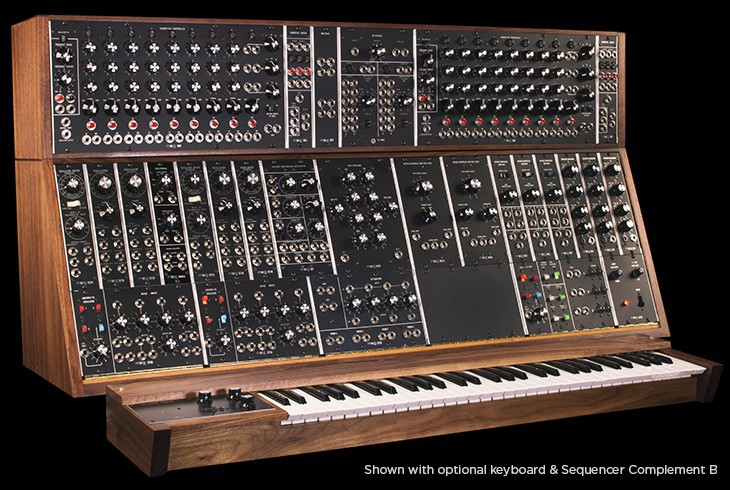
\includegraphics[width = 5in]{MoogSystem35.jpg}
	\caption{Analogue synthesiser - \emph{System 35} (Moog)}
	\label{fig:MoogSystem35}
	% https://www.moogmusic.com/products/modulars/system-35
\end{figure}
%
Digital synthesisers can be much more flexible in their interface, as the audio signals are not passing directily through the controls. Early digital synthesisers had un-user friendly interfaces consising of LCD screens and rows of buttons to alter the parameters, hidden in a series of menus (Fig. \ref{fig:YamahFS1R}). As these interfaces lacked the hands-on control that musicians loved from analogue synths, many digital synths were less popular despite being capable of producing a much wider variety of sounds. Many users found the process of programming these synths to be incredibly frustrating \cite{Synth}. To make the interfaces more user friendly, most digital synths are provided with a set of presets - parameter settings that produce useful sounds - which demonstrate a wide range of the synth's capabilities. %One of the reasons the synthesiser sounds of the 1980s were so simlar to each other, is that many musicians would entirely use the preset sounds, without altering them at all. This is in part due to the novely of the sounds at the time, and in part due to the difficult user interfaces \\
%
\begin{figure}[h] 
	\centering
	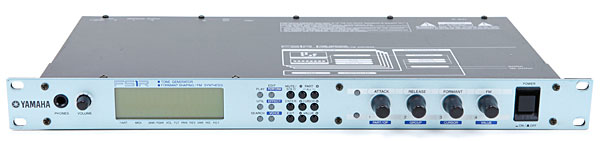
\includegraphics[trim = {0, 0.2cm, 0, 0.5cm}, clip, width = 5in]{yamaha_fs1r.jpg}
	\caption{Digital synthesiser - \emph{FS1R} (Yamaha) \cite{FS1R}}
	\label{fig:YamahFS1R}
	% http://www.vintagesynth.com/yamaha/fs1r.php
	\vspace{-10pt}
\end{figure}\\
Soft-synths have a wide variety of interfaces. Many follow similar design patterns to analogue synths, but with additional interactive elements such as user-drawable envelopes. An example of this is the very popular \emph{Massive} by Native Instruments \cite{Massive} (Fig. \ref{fig:MassiveNI}). Other soft-synths offer much more visual and interactive interfaces, such as \emph{Wavetable} by Ableton \cite{Wavetable} (Fig. \ref{fig:AbletonWavetable}).

\begin{figure}[h] 
	\centering
	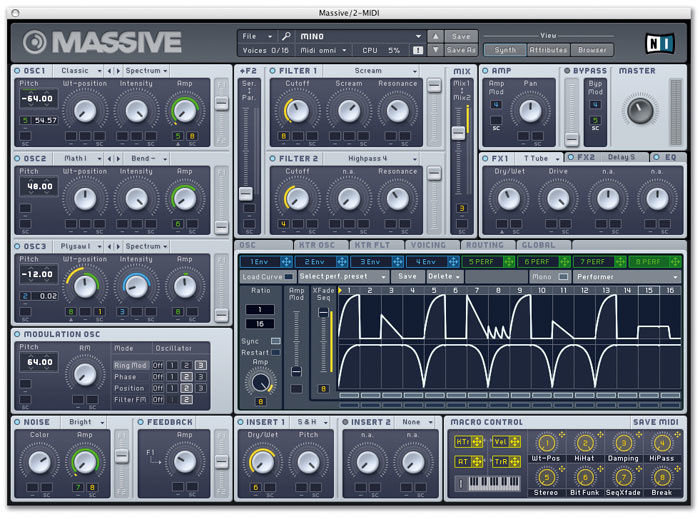
\includegraphics[width = 5in]{MassiveNI.jpg}
	\vspace{-5pt}
	\caption{Software Synthesiser - \emph{Massive} (Native Instruments) \cite{Massive}}
	\label{fig:MassiveNI}
	%https://www.soundonsound.com/reviews/native-instruments-massive
	\vspace{-10pt}
\end{figure}

\begin{figure}[h] 
	\centering
	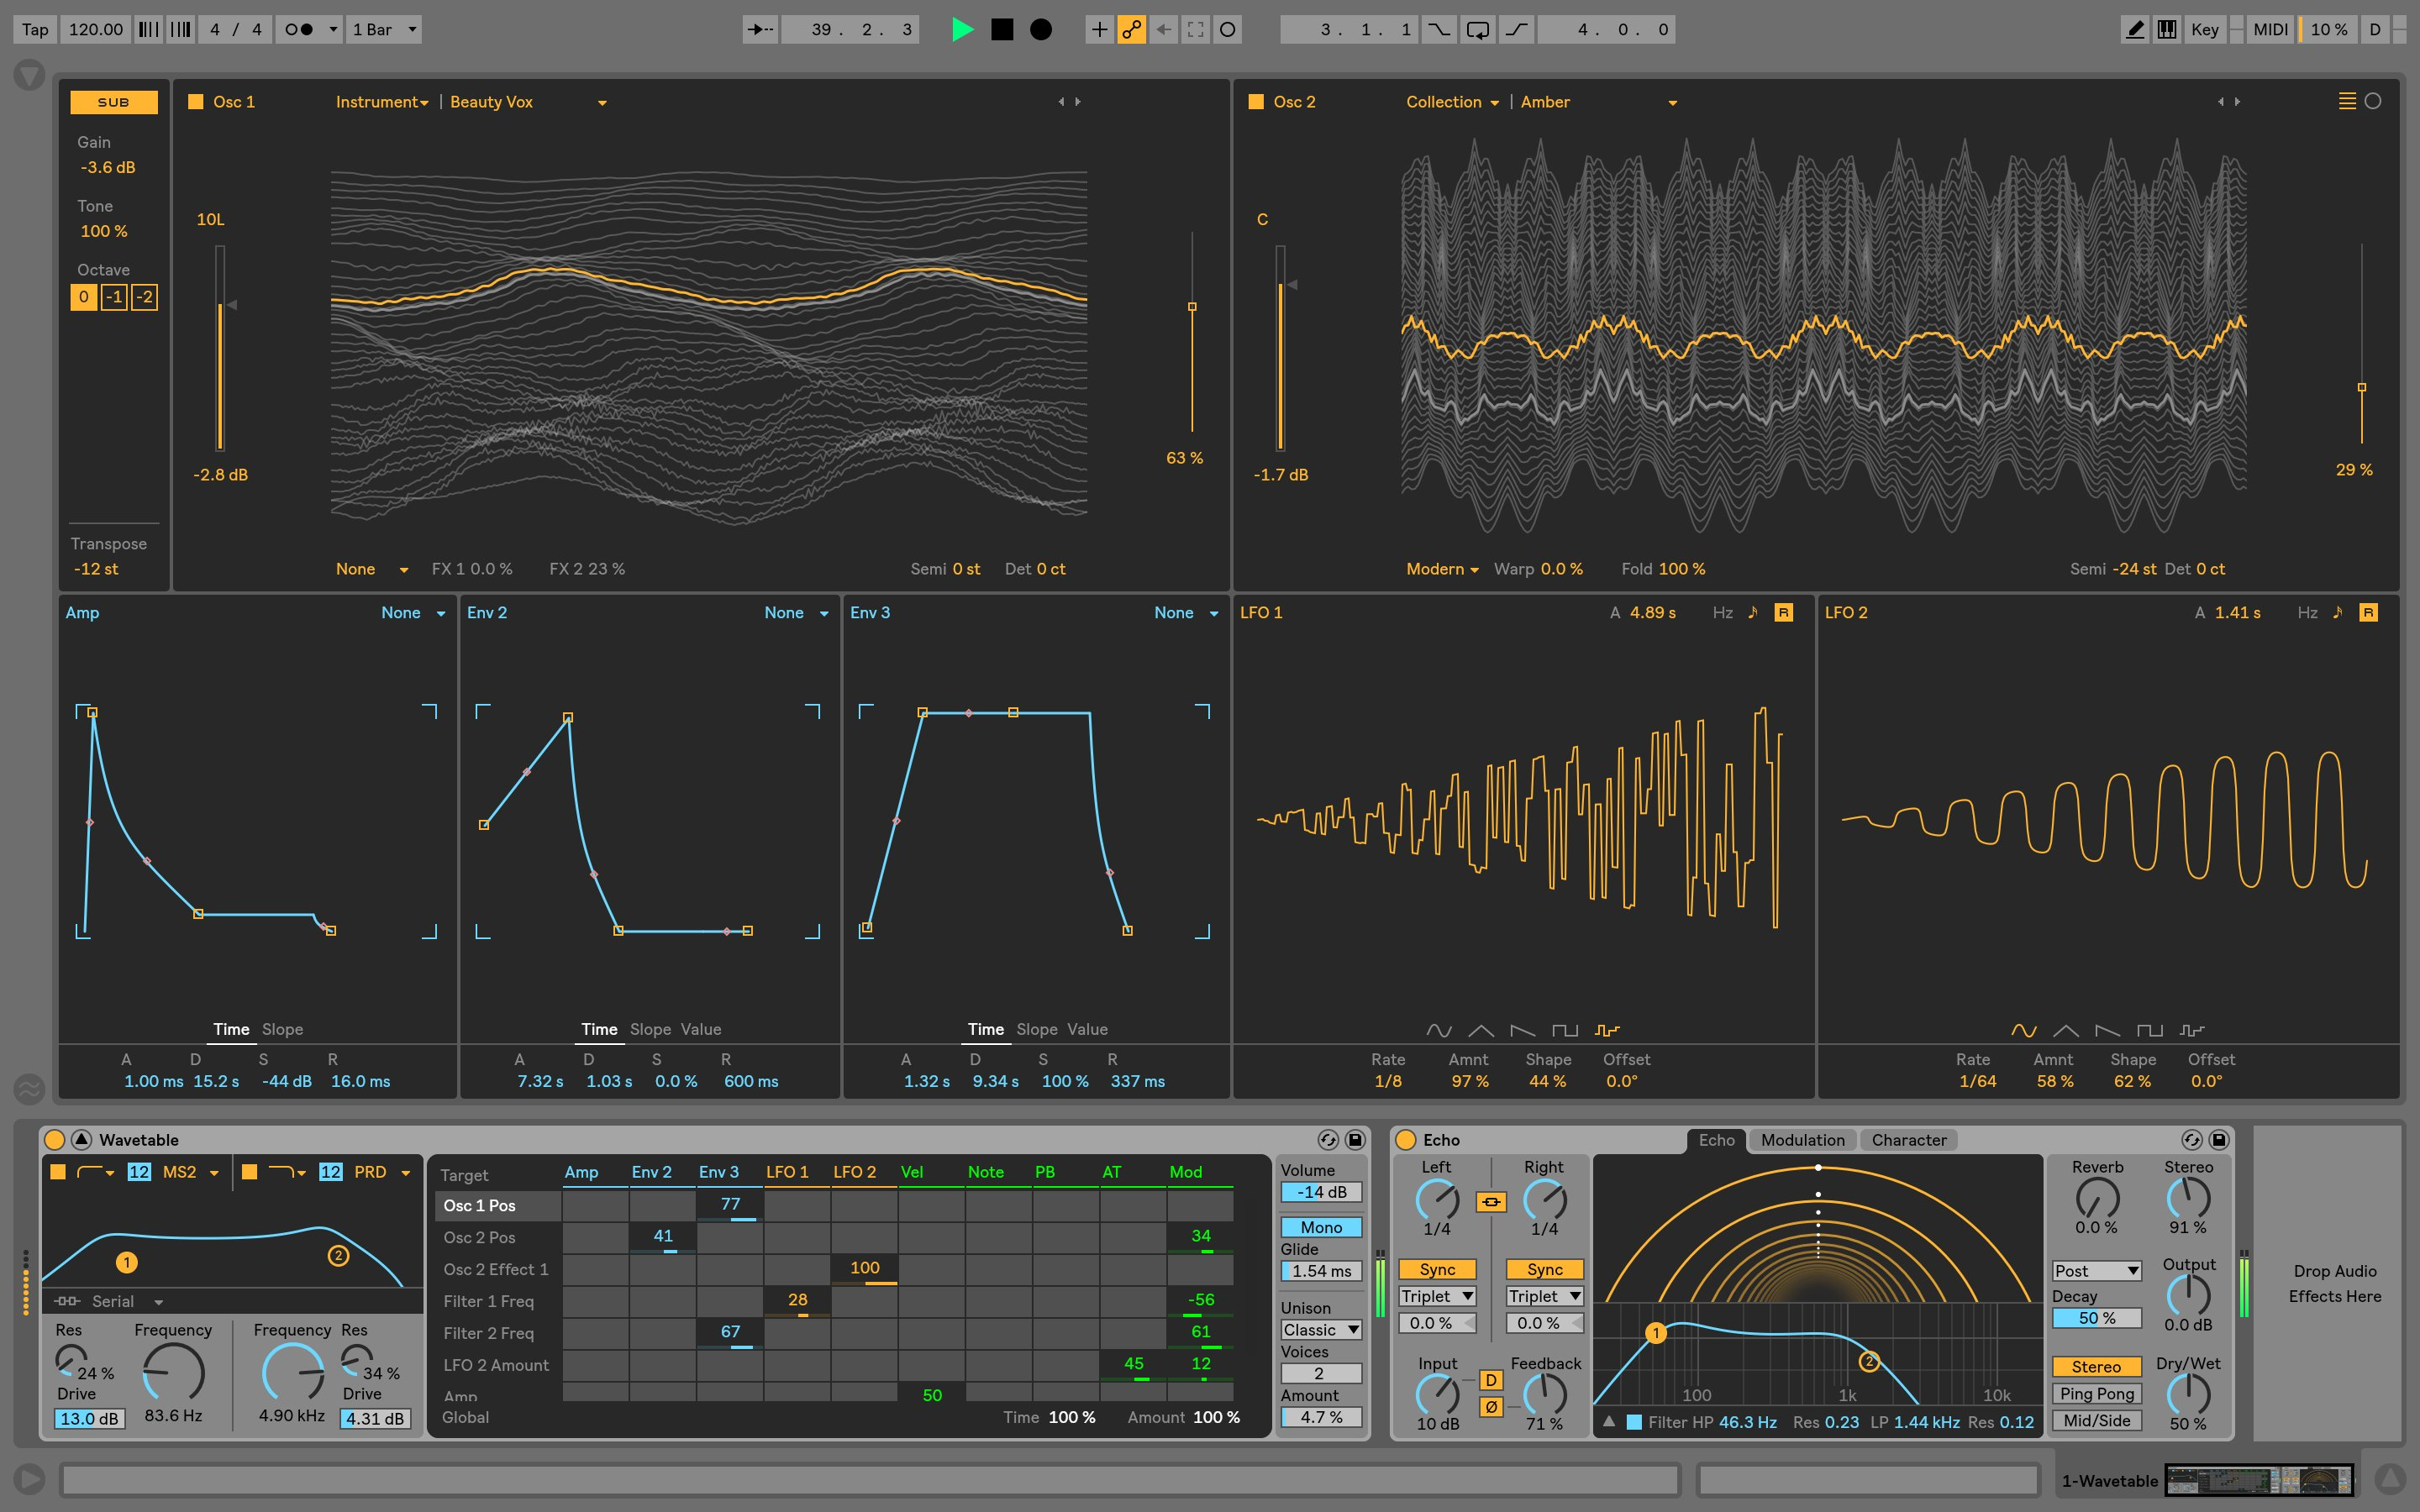
\includegraphics[width = 5in]{AbletonWavetable.jpg}
	\caption{Software Synthesiser - \emph{Wavetable} (Ableton)\cite{Wavetable} }
	\label{fig:AbletonWavetable}
	%https://www.ableton.com/en/packs/wavetable/
\end{figure}

Some soft-synths have modular designs, such as \emph{Modular} by SoftTube, %\cite{SoftTube}
and some even allow users to design synthesis modules from scratch, such as \emph{Max/MSP} and \emph{Supercollider}.

There has been a wide range of reasearch in the Computer Music field in the use of multideminsional controllers, such as the  \emph{Myo}, \emph{Leap Motion} and \emph{Microsoft Kinect}, to control synthesis parameters in real time \cite{ICMC, TubbThesis}, and research into advanced user interaction types, such as waveform blending (see \emph{wavetable synthesis} \cite{Wavetable} and \emph{vector synthesis} ), preset blending \cite{Interpolation}, randomisation of presets, and many more \cite{YeeKing, EvolvedAudioEffects}.  Several studies have applied a variety of machine learning techniques to synthesiser control, as described in the next section.

\section{Using Machine Learning to Control Synthesisers}\label{MachineLearning}
Many users have difficulties programming synths, due to the large amount of technical and creative skill necessary (\cite{YeeKing} \S 4.1.1). There have been several previous attempts to use machine learning to make programming synths easier and more expressive, from both academia and commercial products (\cite{YeeKing} \S 4.1.2).

The Google NSynth project \cite{NSynth}, develops a technique for interpolating between sampled instruments, in the latent space of a \emph{WaveNet Autoencoder} rather than operating directly on the audio recordings. This project has impressive results, but a downside is that it relies upon pre-computing a large database of audio recordings to densely sample the latent space, which are then interpolated for real time playback. Furthermore only 16 instruments were sampled.

\emph{Tone-matching} is an active area of research in which synths are automatically programmed to match a reference audio recording. Common techniques involve using global optimisation techniques, such as genetic algorithms, feed-forward neural networks and gradient methods. This either requires a system which continuously monitors the output of the synth and calculates a sound-based metric to compare to the reference recording's metric, or requires a densely sampled database of metric values over the parameter space of the synth.  The Mel Frequency Cepstrum Coefficient (MFCC) has been identified as the best metric to use, as it is based on human perception \cite{YeeKing}.

Several works have applied \emph{interactive genetic algorithms} to synth programming \cite{EvolutionaryInteractive, GenSynth, GenComparison}. Typically the genetic algorithm produces a variety of presets, and the user acts as the \emph{fitness function}, selecting the best of these to be used for the next iteration. An advantage of using genetic algorithms is that they can be applied to modular synths, allowing the synthesis architecture to mutate. The Blending Interface (\S \ref{sec:BlendingDescription}) has a similar iterative approach, but has been designed so that each iteration can be carried out a lot faster by the user. 

Dimensionality reduction was applied to audio recordings in the \emph{Infinite Drum Machine} \cite{InfiniteDrum}. In this work, \emph{t-Distributed Stochatic Neighbour Embedding} (tSNE) was used to create a two dimensional mapping of a large number of audio recording (samples). An interface based on this mapping was used for sample-selection in a drum machine. \\
The Selection Interface (\S \ref{sec:SelectionDescription}) draws inspiration from this project. It would be possible to carry out the same process for a synth if first an audio recording was taken of each preset. However, the best way to select which audio recording should be taken from each preset is not clear, as different presets respond very differently to the \emph{MIDI Note}, \emph{Velocity}, and \emph{Note Length}. Therefore the best sampling method to accurately characterise a synthesiser preset, in as few audio recordings as possible, is an open research question.\\
In this work a parameter-based approach is taken, to see if similar quality results can be obtained through a statistical analysis of the presets of a synth. This approach has many benefits such as the speed of the mapping, and the amount of storage required.

The \emph{Wekinator} \cite{Wekinator} is an infuential application of \emph{interactive machine learning} (also known as \emph{active learning}) in music, in which expressive control mappings can be generated for many different types of user interaction based on a small number of user supplied training examples. This approach could be used to allow the interface designed in this report to be controlled more expressively, and make it better suited to live performance.
\section{HCI design principles for Creative Musical Interfaces}\label{sec:Tubb}
Several results from the field of \emph{Human-Computer Interaction} (HCI) give useful insights into synth interface design.\\
There are four main types of parameter mapping in synthesier interfaces:\cite{MappingStrategies}
\begin{itemize}
\vspace{-10pt}
\setlength\itemsep{-1.2em}
\item One-to-one: each control dimension is mapped to a single synthesis parameter.
\item One-to-many: one control dimension is mapped to many synthesis parameters.
\item Many-to-one: many control parameters affect one synth parameter.
\item Many-to-many: a combination of the above (known as ‘complex’ mappings).
\end{itemize}
\vspace{-10pt}
Complex many-to-many mappings appear to be the most effective for many users, as well as being more fun and inspiring higher levels of creativity. It appears that they allow users to intuitively learn to navigate the control space. One-to-one interfaces on the other hand require the user to break the creative process into a number of subtasks, and are reported to be confusing and frustrating to use.

In \cite{TubbThesis}, number of guidelines for creative musical interfaces are presented:
\begin{enumerate}
	\vspace{-10pt}
\setlength\itemsep{-1.2em}
	\item \emph{Low dimensionality}: Control devices often have fewer parameters than synthesis algorithms. Given the brain's limited conscious multi-tasking abilities and working memory capacity, simple controllers are preferable.
	\item \emph{Locality}, or distance preservation: Distance travelled in control space, should be reflected in the distance travelled in parameter space, and ideally perceptual distance too.
	\item \emph{Revisitability}: If a point in control space is revisited, the sound should be the same. The location of preset points should be stable.
	\item \emph{Continuity}: If a point is adjacent to another point on the low-dimensional surface, they should be adjacent in the high-dimensional space.
	\item \emph{Smoothness}: Continuous higher derivatives are desirable to eliminate sudden changes in direction, this has relevance to the predictability of a control.
	\item \emph{Linearity}: When a gesture, such as a scroll, occurs it will have a certain effect on the sound. More extreme versions of the gesture should produce more of the same effect. %This property is hard to achieve with any dimensionality reduction method, however smoothness implies some linearity in the immediate neighbourhood.
	\vspace{-10pt}
\end{enumerate}
The Blending Interface (\S \ref{sec:BlendingDescription}) follows all of these design guidelines, and the Selection Interface (\S \ref{sec:SelectionDescription}) follows all except the \emph{Smoothness} condition (due to the sudden jumps between presets). Both are complex many-to many interfaces.

In \cite{TubbThesis}(\S 5.5.3), the EARS model for creative cognition is developed. It describes four modes of creative cognition which can be used to design and evaluate creative interfaces (Fig. \ref{fig:EARSmodel}).
\begin{figure}[h] 
	\centering
	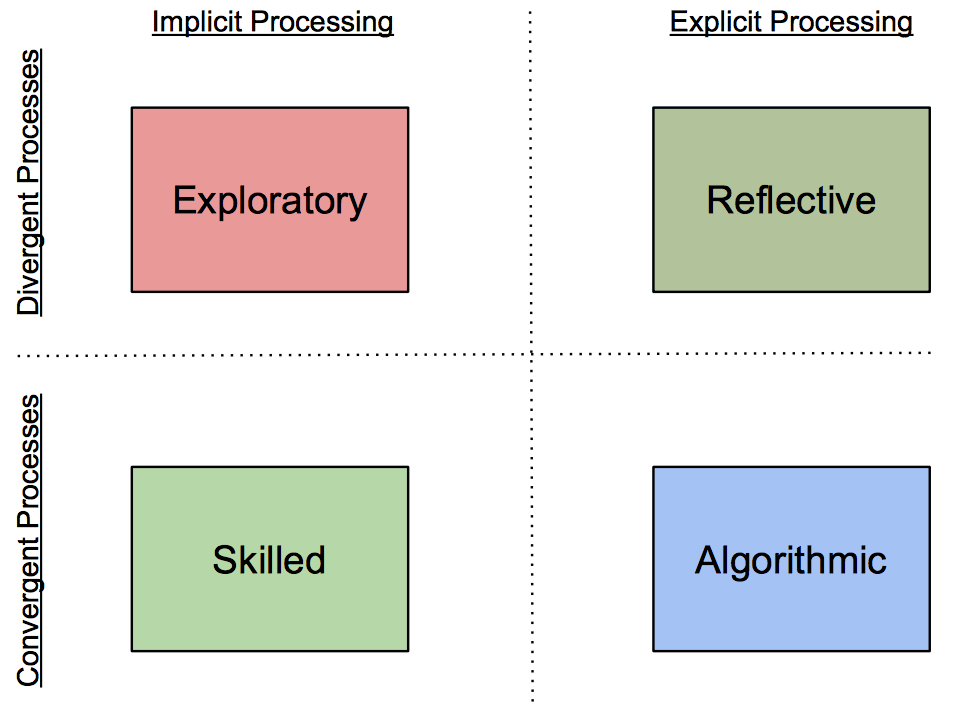
\includegraphics[width = 5in]{EARSmodel.png}
	\caption{The four quadrants formed by drawing distinctions between implicit vs. explicit thinking (left/right) and divergent vs. convergent thinking (top/bottom). \cite{TubbThesis}}
	\label{fig:EARSmodel}
\end{figure}\\
For different creative tasks, interfaces suited to an appropriate mode of creative cognition (Exploratory, Reflective, Skilled or Algorithmic) will be more effective, and it is important for users to be able to easily switch between these different modes. This project's interface is evaluated using this model in Section \ref{sec:EARS}.

%ALSO>>>>>Talk about the stuff about multidemsional controlers having higher thoroughput. - Not sure this is relevant

\chapter{Description of Synthesiser Algorithm}
\section{Description}
 It was necessary to choose a synth to use, in order to develop the interface. To remove some of the complexities of communicating with commercial synths, a purpose built synth was made in the programming language \emph{Supercollider}.
A \emph{six operator phase modulation} (PM) synth was created,\footnote{PM synthesis is very closely related to FM synthesis \cite{FM}, and the names are often used interchangeably.} loosely based on the Yamaha \emph{DX7}, and was designed to be representative of typical commercial soft-synths.
 
The synthesis algorithm uses the \emph{FM7 UGen} for Supercolldier \cite{UGen}. This implements six \emph{operators}\footnote{A general term for waveform generators in PM synthesis. In this case, sine-wave generators are used.} with independent amplitudes and frequencies, whose outputs can be used to modulate each other's phase. This is described by the following discrete-time equation: 
\begin{equation}
y_i[t+1] = a_i\sin(2\pi T f_i + \sum_{j = 1}^{6} y_j[t] m_{ij})
\end{equation}
where $T$ is the sampling interval,  $y_i[t]$ is the output of operator $i$ at time $t$, $a_i$ and $f_i$ are the amplitude and frequency of operator $i$ and $m_{ij}$ is a scalar parameter determining the level of phase modulation from operator $j$ to operator $i$. This is a very flexible sound generation algorithm which can create a large number of different sounds. \\
The full synthesis architecture (Fig. \ref{fig:SynthSchematic}) can be described as follows.\\
 A \emph{MIDI Note ON} message is received with a musical note number $N$ and a velocity $V$. This triggers the sound generations process for this particular note. the note number $N$ is converted into a base frequency $F$. The frequency of each operator is set using the equation: 
 \begin{equation}
	f_i = Ff_i^{coarse}(1+f_i^{fine})
 \end{equation}
The coarse frequency parameter $f_i^{coarse}$ for operator $i$ can take discrete values \{0.5, 1, 2, 3, \dots\}, allowing the operators to set to different harmonics of the base frequency. The fine frequency parameter $f_i^{coarse}$ can take any value in the range [0,1], and is used to detune operators away from the perfect harmonic ratios. This is the approach usually taken in typical synthesisers when setting frequencies, as the fine frequency values are typically very small.\\
The base frequency $F$ can be continually modulated by the \emph{MIDI PitchBend} control, and by a vibrato envelope (an exponential ramp from a start frequency and amplitude to an end frequency and amplitude, over a time period in the range [0, 20] seconds).

The operators are then continuously \emph{amplitude-modulated} by two \emph{low frequency oscillators} (LFOs), and a \emph{modulation envelope}, as described by the discrete-time equation:
 \begin{equation}
a_i[t] = (1 + \mathrm{LFO}^a[t]*\mathrm{lfo}^{a}_i)*(1 + \mathrm{LFO}^b[t]*\mathrm{lfo}^{b}_i)*(\mathrm{ENV}^{mod}[t]*\mathrm{env}^{mod}_i + (1-\mathrm{env}^{mod}_i))
\end{equation}
where  $a_i[t]$ is the amplitude of operator $i$, $\mathrm{LFO}^a$ and $\mathrm{LFO}^b$ are the LFOs' output values, $\mathrm{ENV}[t]$ is the modulation envelope's output value, all at time $t$. $\mathrm{lfo}^{a}_i$, $\mathrm{lfo}^{b}_i$, and $\mathrm{env}^{mod}_{i}$ are parameters which determine how much operator $i$ is modulated by the respective signals. \\
LFO A is a zero-mean \emph{triangle wave oscillator} with a frequency in the range [0, 20\si{\hertz}], amplitude in the range [0, 1], and phase spread in the range [0, 1] (a parameter which allows the LFO's initial phase to be randomly varied). LFO B is a zero-mean \emph{square wave oscillator} with a frequency in the range [0, 20\si{\hertz}], amplitude in the range [0, 1], and pulse width in the range [0, 1]. The modulation envelope is an \emph{ADSR  envelope generator}\footnote{A commonly used type of envelope generator with the parameters Attack, Decay, Sustain and Release.}, which is triggered by the MIDI Note ON message.


After amplitude modulation, the operators amplitudes and frequencies are used as inputs to the previously described phase modulation algorithm. The six outputs from this algorithm are then mixed together, and multiplied by the \emph{amplitude envelope} (another ADSR envelope generator) to form the output signal: $Y[t] = \mathrm{ENV}^{amp}[t]*\sum_{i=1}^{6}y_i[t]*a_i^{output}$, where $a_i^{output}$ is the Output Level parameter for operator $i$.

The synth has 96 parameters, as described in Table \ref{tab:Params}. All of the parameters can be easily adjusted in real time, by sending messages over \emph{Open Sound Control (OSC)} \cite{OSC}, a UDP based protocol for inter-application communication.

35 presets were created for this synth, to give a selection of the different sounds the synth can make, and to provide dataset to design the interface with.
\begin{figure}[h] 
	\centering
	\hspace*{-1cm}
	\includegraphics[width = 7in]{SynthSchematic.png}
	\caption{Software Synthesiser Schematic - a 6 operator Phase Modulation synthesiser, with two LFOs, and seperate envelope generators for modulation, amplitude and vibrato. Implemented in \emph{Supercollider} with 96 parameters controlable in real time over the \emph{OSC} protocol.}\label{fig:SynthSchematic}
\end{figure}

\def\arraystretch{1.5}
\begin{table}[]
	\hspace{-2em}
	\begin{tabular}{|l|l|l|l|l|}
		\hline
		\textbf{Parameter Group}                	 & \textbf{Parameter}     & \textbf{Domain}            & \textbf{Time/Timbre} & \textbf{Weighting} \\ \hline
		Phase Modulation         						& 36 x $m_{ij}$               & $[0, 10]$                  		& Timbre                	& 3									\\ \hline
		Coarse Frequency                            	& 6 x $f_{i}^{coarse}$     & $\{0.5, 1, 2, 3, 4, ...\}$ & Timbre                	& 10									  \\ \hline
		Fine Frequency                                 	   & 6 x $f_{i}^{fine}$         & $[0, 1]$                   		& Timbre                	& 10									  \\ \hline
		Output Level                                  		& 6 x $a_{i}^{output}$     & $[0, 1]$                   	  & Timbre                	& 3								    	\\ \hline
Modulation Envelope Amount                       & 6 x $\mathrm{ENV}_{i}^{mod}$   & $[0, 1]$                   	     & Timbre                  & 1		  \\ \hline
		LFO A Depth                                    		& 6 x $\mathrm{LFO}_{i}^{a}$         & $[0, 1]$                   	   & Timbre                  & 1				\\ \hline
		LFO B Depth                                    		& 6 x $\mathrm{LFO}_{i}^{b}$        & $[0, 1]$                   	   & Timbre                  & 1				\\ \hline
		\multirow{3}{*}{LFO A}      					& Rate                    		& $[0, 20]$ Hz               	 & \multirow{3}{*}{Time}& \multirow{3}{*}{3} \\
																	  & Amplitude               	& $[0, 1]$                   		&                      				& \\
																	  & Phase Spread         	& $[0, 1]$                   		&                       			&\\ \hline
		\multirow{3}{*}{LFO B}      					& Rate                    		& $[0, 20]$ Hz               	& \multirow{3}{*}{Time}& \multirow{3}{*}{3} \\
																	  & Amplitude               	& $[0, 1]$                   		&                       			&\\
																	  & Pulse Width                & $[0, 1]$                   		&                       			&\\ \hline
		\multirow{5}{*}{Amplitude Envelope}    & Attack (A)       				& $[0, 10]$ seconds        & \multirow{5}{*}{Time}& \multirow{3}{*}{10} \\
																	  & Decay (D)               		& $[0, 10]$ seconds         &                       			&\\
																	  & Sustain (S)             	 	 & $[0, 1]$                   		&                       			&\\
																	  & Release (R)             		& $[0, 10]$ seconds        &                       			&\\
																	  & Curve                   	   	   & $[-5, 5]$                  	&                       			&\\ \hline
		Modulation Envelope        						& Same as previous           &                            			& Time              	& 10									\\ \hline
		\multirow{6}{*}{Miscellaneous}             & Vibrato Start Amt.    		  & $[0, 1]$                   	& \multirow{6}{*}{Time}& \multirow{3}{*}{1} \\
																	  & Vibrato End Amt.	         & $[0, 1]$                   		&                       			&\\
																	  & Vibrato Start Freq.			  & $[0, 20]$ Hz               &                       			&\\
																	  & Vibrato End Freq.		      & $[0, 20]$ Hz               &                       			&\\
																	  & Vibrato Time            		& $[0, 20]$ seconds      &                       			&\\
																	  & Stereo Spread           	  & $[0, 1]$                   		&                       			&\\ \hline
	\end{tabular}
\caption{Synthesiser Parameters}
\label{tab:Params}
\end{table}

\section{Design choices and justification}\label{sec:SynthDescription}
Typical commercial synths have a large number of parameters\footnote{For example, the \emph{Yamaha DX7} has 126 parameters, and  \emph{Omnisphere 2} has several thousand parameters}, which can be discrete or continuous, and are usually constrained within a range. Some synths have Modular or Semi-Modular architectures, which allow for considerable flexibility, but due to the combinational explosion of number of parameter combinations, and difficulty blending between presets, this type of architecture is not addressed in the work.
Some synths use short audio recordings, known as samples, as part of their sound creation algorithm. This creates difficulties blending between presets, so this type of architecture will not be considered in this work. (However both of these types of synths would be interesting to try as a follow up work).

This work is aimed at analogue-style synths, in which there are a medium number of parameters with a fixed internal routing. Effects modules, such as reverb, delay and chorus have not been included in the synth, as these can easily be added to the signal chain by users. Effects modules also tend to be much easier to control than synths, as they typically have fewer, and more intuitive parameters. Effects modules are typically chained together in series, with no feedback, so each effect module is a seperate transfer funtion, with no covariance between the parameters.

The synth features a combination of continuous and discrete parameters, all of which are bounded. Common bounds are: $[0, 1]$, $[0, k]$ and $[-k, k]$, where $k \in \mathbb{R}^+ $ (See Table \ref{tab:Params}).

The DX7 was chosen as a base synth as although it is a very powerful, it is notoriously difficult to use due to the unintuitiveness of the phase modulation algorithm. An improved interface has the ability to open up FM synthesiser programming to non-expert users. %WORK ON THIS

The synth was designed to have access to as wide a range of sounds as possible with as few parameters as possible. For example instead of having a separate envelope generator for each oscillator as the  DX7 does, only two envelopes were included, with an adjustable amount per operator. The synth has 96 total parameters, compared to the 126 of the DX7, but it can replicate most of the useful sounds of a DX7. Despite aims to reduce parameter count, there are still many redundant parameters in most presets for this synth. For example, if the amplitude of one of the LFOs is set to zero, all of the other parameters to do with the LFO will have no effect on the sound. This is a common feature with synths, and presents a challenge when trying to learn useful information from the parameters.

In Yee King's thesis \cite{YeeKing}, a similar FM7 Ugen based Supercollider synthesiser was used, but no envelopes or LFOs were included, so that it was limited to producing sounds with a static timbre. Whilst this had advantages for the timbre mapping approach of the work, it resulted in a synthesiser that was not very representative of ones typically used, as envelopes are such an important part of designing sounds. 

As this synth has six identical operators which can be configured in any combination, there is lots of possible \emph{permutation ambiguity}: if two operators have all of their parameters switched, the sound will remain identical. This presents a challenge (\S \ref{sec:PermutationAmbiguity}) as two presets can have very different parameters despite having the same sound.

\chapter{Description of Full Interface}
The full interface developed in this report is a combination of three interfaces. Each has the ability to vary the entire set of parameters, and produce a wide variety of sounds, but they are designed to complement each other as well as possible. The user can easily move back and forth between the different interfaces. The interface is designed to use as little information about the synth as possible, so that it can be easily applied to other synths. A video of the full interface can be viewed at (LINK), and a working demo can be downloaded from (LINK).
%\vspace{-15pt}
\section{Traditional Interface}
The \emph{Traditional Interface} is designed to be representative of a typical soft-synth interface. It has a knob or slider for each synthesis parameter, and has interactive visualisations for some parts of the architecture (namely the envelopes and LFOs). The interface is arranged in three seperate pages, two of which are shown in Fig. \ref{fig:TraditionalInterface}. 
If the full interface were to be extended to work with any VST, the traditional interface would be replaced by the VST's user interface. 
\begin{figure}[h!] 
	\vspace{-5pt}
	\centering
	\hspace*{-0.2cm}
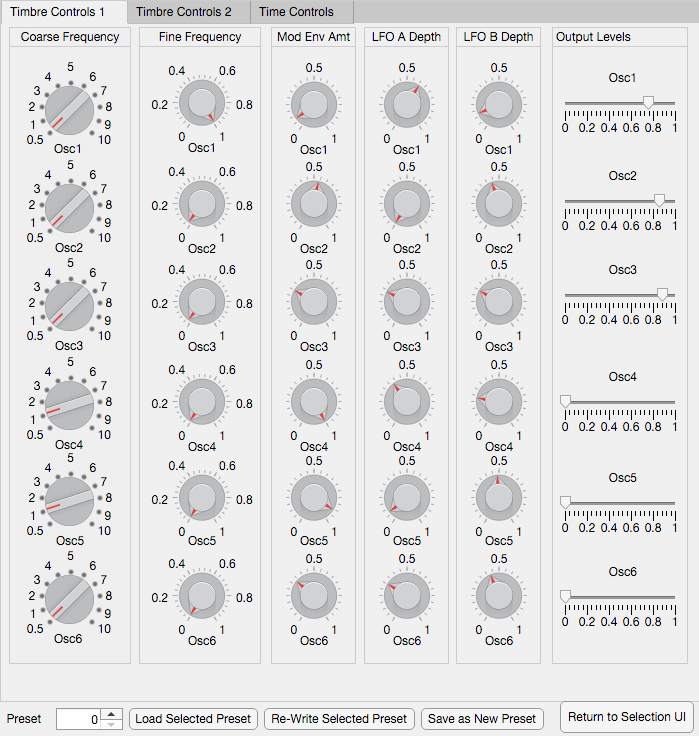
\includegraphics[width = 3in]{TraditionalUI1.png}
\hspace*{0.2cm}
	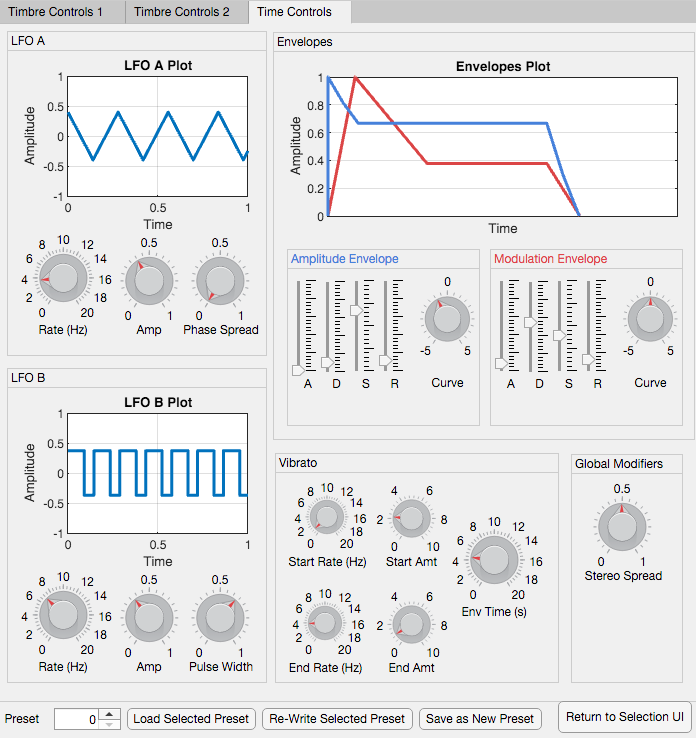
\includegraphics[width = 3in]{TraditionalUI3.png}
	\caption{Traditional Interface - `Timbre Controls 1' and `Time Controls' pages}
	\label{fig:TraditionalInterface}
	\vspace{-20pt}
\end{figure}

\section{Selection Interface}
Typical soft-synths are supplied with a large number of presets, which are usually named and arranged into categories. They are usually displayed in a list which can be searched by name, or split into category. In many soft-synths, each preset is given a set of \emph{Macro Controls} (usually eight), each of which vary one or more parameters, and aim to give the user a quick way to fine-tune the presets to their needs.\\
The \emph{Selection Interface} is a new approach to displaying presets, arranging the presets as cells of a \emph{2D Voronoi diagram} \cite{Voronoi}, such that similar presets are close to each other and coloured similarly. The presets can quickly be compared by moving the mouse around the diagram, and presets are selected by clicking on the cells. Once a preset is selected it can be edited by Macro Controls. 
The presets have been divided into a number of categories. Clicking the category buttons at the top of the interface highlights the selected category (Fig. \ref{fig:PCAInterface}). By clicking the `Display Mode' button, it is also possible to limit the presets displayed to just the selected category(s), displayed in a recalculated Voronoi diagram.\\
Both the 2D spacing of the presets, and the mapping of the Macro Controls are calculated automatically from the set of presets' parameter values using Principal Component Analysis.

\begin{figure}[h] 
	\centering
	\hspace*{-0.2cm}
	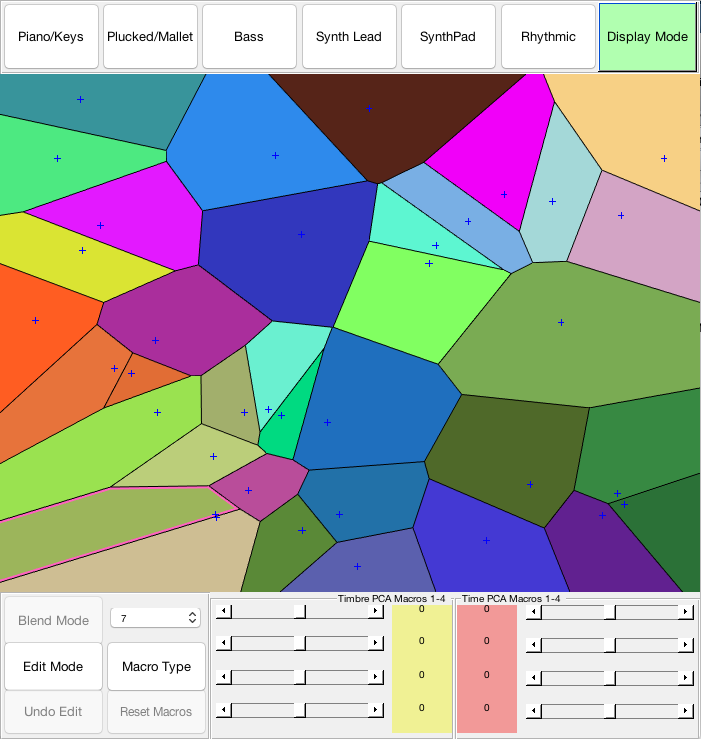
\includegraphics[width = 3.0in]{PCAInterface1.png}
	\hspace*{0.1cm}
	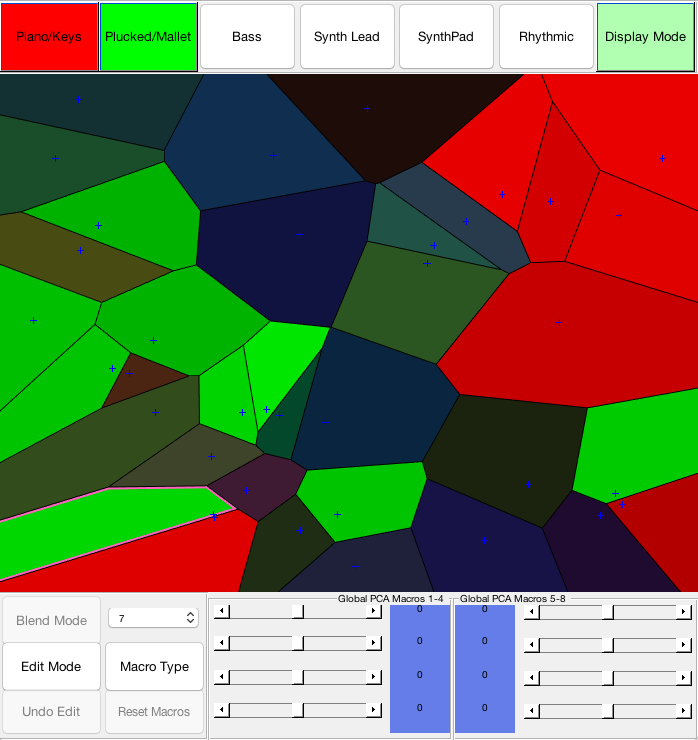
\includegraphics[width = 3.0in]{PCAInterface2.png}
	\caption{PCA Interface - Normal View, and Category Highlight View}
	\label{fig:PCAInterface}
\end{figure}

\section{Blending Interface}
Preset Blending is a popular approach in synth interface design, where new presets are created by a linear combination of presets.\footnote{For example, the \emph{Alchemy} and \emph{FM8} soft-synths allow preset blending, and the  \emph{Nodes} object in \emph{Max/MSP} is a commonly used implementation of preset blending.} The \emph{Blending Interface} extends this approach.

Three initial presets (A, B, C) are selected, and are placed on the corners of a triangle at the centre of the interface (Fig. \ref{fig:BlendingInterface}). As the cursor moves over the interface, a new preset is created as a weighted sum of the three presets, based on proximity to the corners. Once the user finds the optimal preset in the space, the user clicks. The preset clicked on then becomes the preset A (i.e is placed on the bottom corner of the triangle), and a new preset B and C are generated with a novel algorithm (\S \ref{sec:PresetGeneration}). \\
This process can repeat as many times as desired, allowing the user to keep searching through the parameter space.\\
If the user clicks on the `Pause on Selected Preset' button, they are shown an interactive display of their past preset choices, which they can use to return to previously selected settings and resume searching. It is also possible to select three of the previous presets, and assign them to preset A, B and C.
The user has the option to freeze sections of the parameter space (Fig. \ref{fig:FreezeParams}) which helps the search be more fine tuned to their needs.
The colours of the Blending Interface are calculated to be consistent with the Selection Interface.
\begin{figure}[h] 
	\centering
	\hspace*{-0.2cm}
	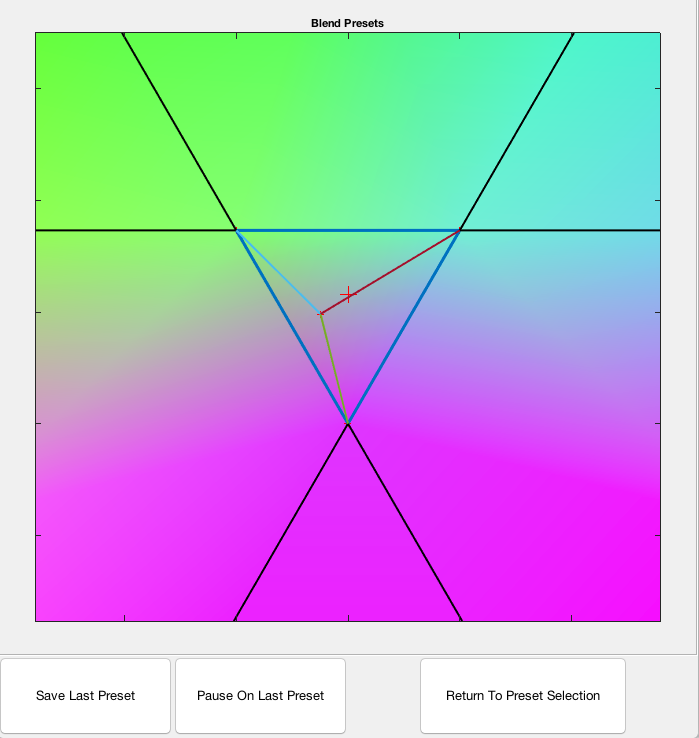
\includegraphics[width = 3.0in]{BlendingInterface1.png}
	\hspace*{0.2cm}
	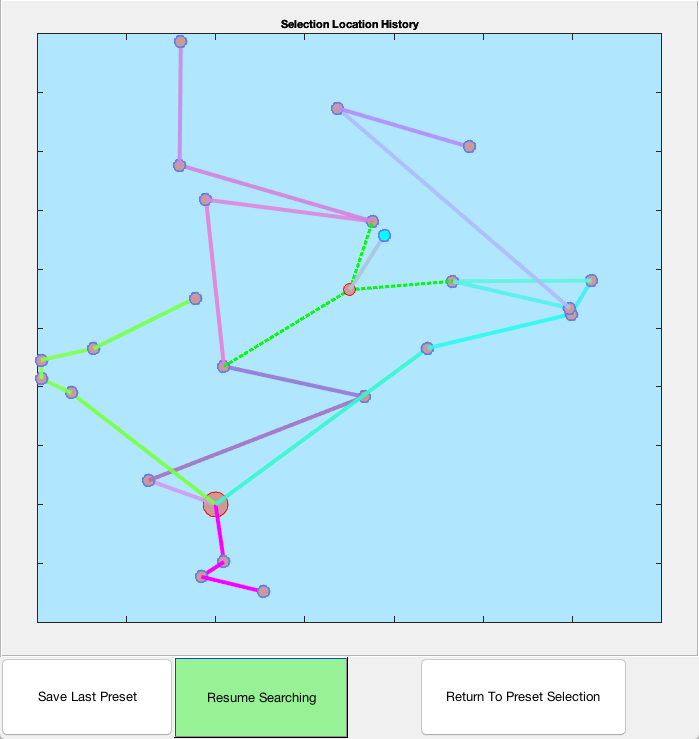
\includegraphics[width = 3.0in]{BlendingInterface2.png}
	\caption{Blending Interface - Normal View, and Selection History View}
	\label{fig:BlendingInterface}
\end{figure}

\section{How the Interfaces are Combined}
When the application is started, the Selection Interface is displayed first. Once a preset has been selected and possibly modified with the Macro Controls, the user has the option to click the `Edit Mode' button, which opens the Traditional Interface, allowing the currently selected preset to be further modified. The user can move back to the Selection Interface by clicking the `Return to Selection UI' button. The varied preset is displayed on the Selection Interface with a marker, attatched to the original preset, which is positioned and coloured to be consistent with the PCA mapping (Fig. \ref{fig:CombinedInterface}). To undo the edits made to the preset the user can click the `Undo Edit' button. In this way the user can move back and forth between the Selection and Traditional interfaces as often as desired.

Once three presets have been selected, the user has the option of clicking the `Blend Mode' button which opens the Blending Interface, and assigns the three selected presets to A, B and C. The user can then use the Blending Interface for as long as necessary, and then click the `Return to Preset Selection' button. This time another marker is created, with dotted lines to the 3 initially selected presets. 
This marker can then be used in the same way as the cells of the Voronoi diagram, i.e it can be previewed by clicking, selected by double clicking, and can be edited with the Macro Controls or the Traditional Interface.

 Parameter visualisations are displayed alongside all of the interfaces to give the user more feedback of the changes they are making with the interface, and to aid in understanding the synthesis algorithm. These are shown on the left and bottom sides of the interface in Fig. \ref{fig:CombinedInterface}.
\begin{figure}[h] 
	\centering
	\hspace*{-1.5cm}
	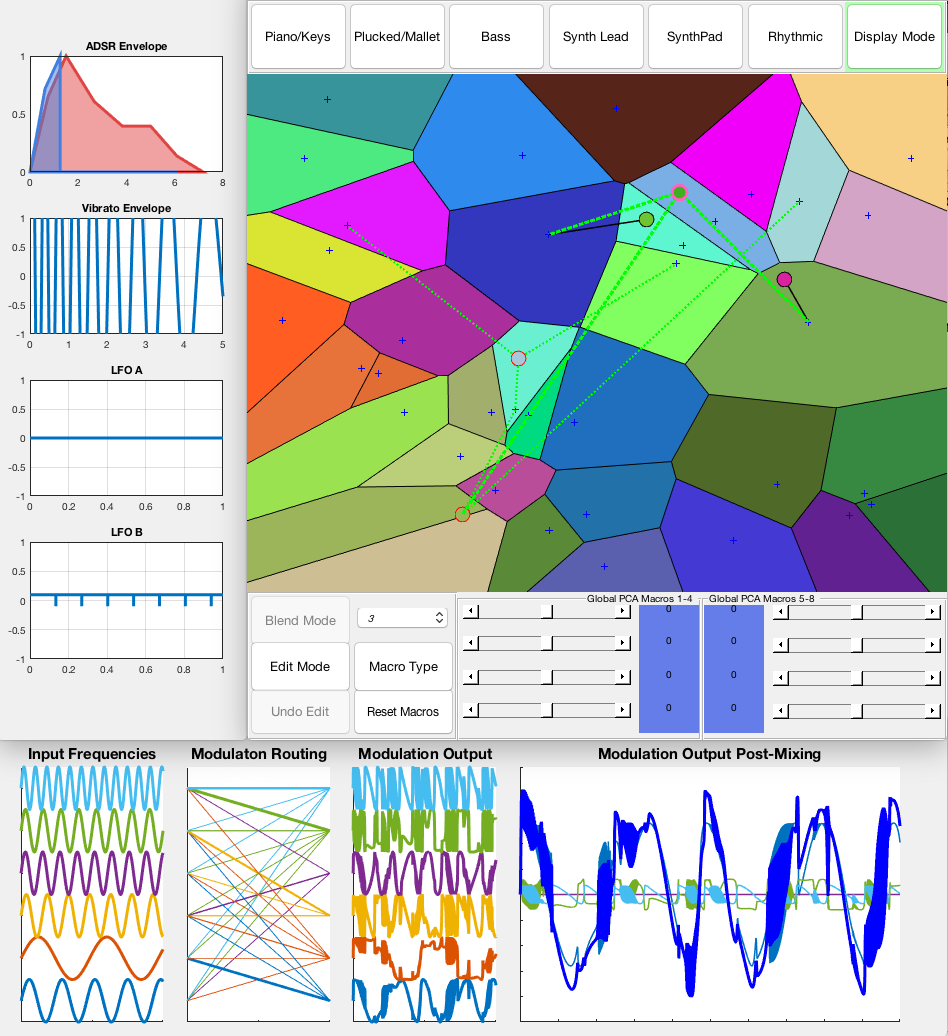
\includegraphics[width = 7.5in]{CombinedInterface1.png}
	\caption{Combined Interface - PCA view. The top right corner of the interface can be swapped for the Traditional Interface and the Blending Interface. The parameter visualisations on the left and bottom sides are common to all three interfaces. The combined preset markers are shown on the Selection Interface, as circles connected to dotted lines.}
	\label{fig:CombinedInterface}
\end{figure}

\chapter{Design and Evaluation of Interfaces}
\section{Traditional Interface}
%\subsection{Detailed Description}
\begin{wrapfigure}{r}{0.5\textwidth}
		\vspace{-30pt}
	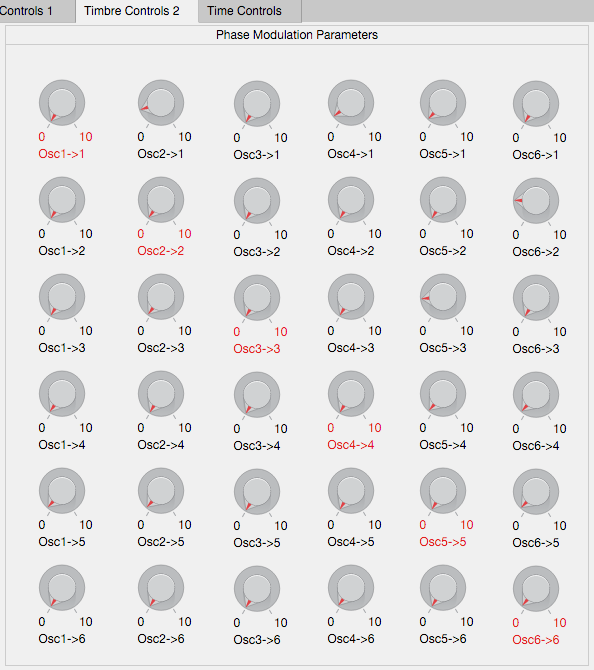
\includegraphics[width = 3.5in]{TraditionalUI2.png}
	\caption{Trad. Interface - 'Timbre Controls 2'}
	\label{fig:TraditionalInterface2}
	\vspace{-70pt}
\end{wrapfigure}
This interface was created in the MATLAB App Designer toolbox. As the parameters are varied, they are sent in real time over OSC to the synth.
\subsection{Strengths}
A skilled user can use knowledge of synthesis to construct any preset they can conceive of. The entire parameter space can be searched. Especially effective for more intuitive sections of the synth architecture, such as the LFOs and envelopes.
\subsection{Weaknesses}
Even if the user knows exactly what each parameter should be set to, it still takes several minutes to go through all of the 96 knobs and set them to the correct value. This is studied in detail in Section \ref{sec:TradEval}, which shows that the order at which the parameters are visited is crucial to the speed of the interface: if they are visited in a random order, the interface is very slow. Parts of the synthesis architecture are non-intuitive and fiddly to use, in particular the 36 phase modulation routing parameters shown in Figure \ref{fig:TraditionalInterface2}. If the user doesn't know exactly what they want, or how to acheive a particular sound, this interface can be extremely inefficient and frustrating.\footnote{For detailed evaluation of similar interfaces, see \cite{MappingStrategies, TubbThesis, YeeKing}.}
\pagebreak
\section{Selection Interface}\label{sec:SelectionDescription}
%\subsection{Detailed Description}
This interface was created as a Matlab figure-based application. A key technical detail of this interface is the choice of mapping function from the high dimensional parameter space to the 5-dimensional XY-RGB space of the interface. Many dimensionality reduction techniques could be used for this, such as \emph{tSNE} (used in \cite{InfiniteDrum}), \emph{Linear Discriminant Analysis}, and \emph{Autoencoders}. The simplest dimensionality reduction technique was chosen to try first: \emph{Principal Component Analysis} (\emph{PCA}). It is linear, non-parametric and has a closed-form solution, making it reliable and simple to implement. Other techniques could be investigated as a follow-up work.
\subsection{Principal Component Analysis}
PCA finds an optimal linear transformation of a dataset onto a set of decorrelated orthogonal basis vectors known as \emph{principal components}. This transformation is optimal in the sense that it diagonalises the covariance matrix of the transformed dataset. 
The principal components are calculated as the eigenvectors of the covariance matrix $\vec{C}_x = \frac{1}{n-1}\vec{X}\vec{X}^T$, where $\vec{X} = [\vec{P}_1, \vec{P}_2, \dots \vec{P}_n]^T$, $\vec{P}_i$ are the individual presets, and $n$ is the number of presets.\\
The eigenvalues of $\vec{C}_x$ are the variances of each component, and the principal components are arranged in order of decreasing variance.
Most of the variance of a dataset typically lies in the first few components, and hence by only using these components, dimensionality reduction is acheived \cite{PCA}. The \emph{PCA score} for a preset is calculated by projecting the preset onto a particular principal component.\\
PCA makes the assumption that directions with large variance correspond to directions of interest. In the case of a synthesiser preset dataset, this assumption is reasonable, as the data has high signal to noise ratio (although this may be affected by permutation ambiguity).\\
PCA is affected by the relative scaling of the parameters in the dataset. This can be accounted for by inversely weighting each parameter by its variance before applying PCA. However, no conclusive evidence was found to show that this is worth doing for our particular dataset.\\
There are several extensions to PCA including \emph{kernel PCA} which generalises PCA to the non-linear case. \emph{Sparse PCA} is another of such extensions, which aims to find principal components which have as few non-zero variables as possible. This is of special interest to the Macro Controls of the Selection Interface, as if each macro control only varies a subset of the parameters, it may make the Macro Controls more intuitive to users.
\subsection{Global PCA vs Time/Timbre PCA}\label{sec:GlobalTimeTimbre}
The PCA is calculated in two different ways for different sections of the interface. In \emph{Global PCA}, each of the $36$ presets' $96$ parameters arranged in a $36 \times 96$ array. PCA is carried out on this array to produce the Global principal components. 
\\
In \emph{Time/Timbre PCA}, the $96$ parameters are partitioned into two sets: $72$ which affect timbre, and $24$ which affect variation of the sound over time (I.e all of the envelope and LFO parameters). PCA is then carried out seperately on the resulting  $36 \times 72$, and $36 \times 24$ arrays to produce the Time principal components, and the Timbre principal components. 
\\
The Global principal components are used for the XY-RGB mapping of the Voronoi diagram, the Global PCA Macros, and for colouring the Blending Interface. The Time/Timbre PCA principal components are just used for the Time/Timbre Macro Controls.

The user is given the option to switch between the Global, and Time/Timbre Macro Controls. The Global controls allow a greater amount to the space to be searched, but the Time/Timbre controls can be more understandable. See Section \ref{sec:SelectionEval} for an evaluation of the two  types.\\
The Macro controls are the same for all presets, but centered on the currently selected preset. i.e. they allow a relative change of parameters not an absolute parameter change. A possible extension is to create a unique set of macro controls for each preset, which may make macro controls more useful, but at the sacrifice of consistency between presets.

Another possible extension to this approach is to allow parameter freezing (as in the Blending Interface, \S \ref{sec:BlendingDescription}), and automatically recalculate the Macro Control mapping based on the currently unfrozen parameters.


\subsection{PCA + Histogram Equalisation Description}
When using the Global PCA scores to calculate the XY-RGB position of each preset in the Voronoi diagram, there are some undesirable characteristics of the mapping produced. The sizes of the cells varies dramatically, and the majority of the presets usually get compressed into one of the corners (Fig. \ref{fig:histEqBefore}). This is because PCA is linear, and so outliers will skew the diagram. After rescaling to $[-1, 1]$ to fit in the diagram, the inliers will be compressed to a small range. A similar effect occurs with the colour mapping, causing many of the colours to be similar to each other, minimising the dynamic range of the diagram. Research in the field of user interface design shows that users usually associate larger icons with greater importance (REFERENCE), therefore it would be preferable for all the presets to be of a similar size, so as not to give uninteded meaning to particular presets.\\
To fix this issue, a variant of an image processing method known as \emph{histogram equalisation} \cite{HistogramEqualisation} was used, resulting in the mapping shown in Fig. \ref{fig:histEqAfter}.

\begin{figure}
	\centering
	\begin{subfigure}[b]{0.45\textwidth}
		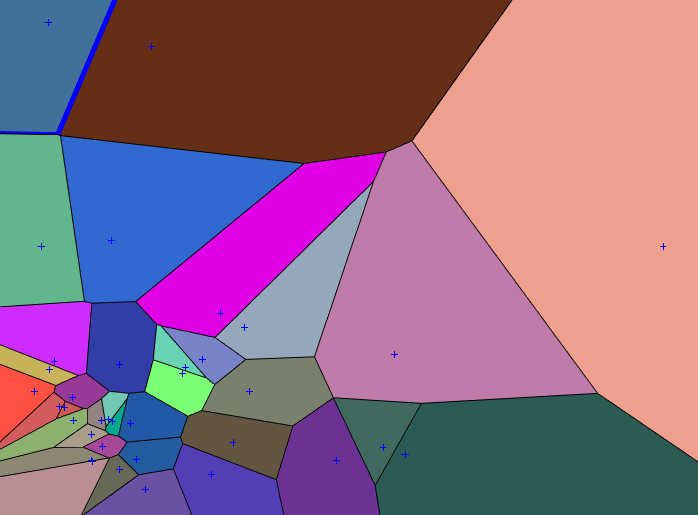
\includegraphics[width=\textwidth]{PCAInterfaceHistEqBefore.png}
		\caption{PCA alone.}
		\label{fig:histEqBefore}
	\end{subfigure}
	~ %add desired spacing between images, e. g. ~, \quad, \qquad, \hfill etc. 
	%(or a blank line to force the subfigure onto a new line)
	\begin{subfigure}[b]{0.45\textwidth}
		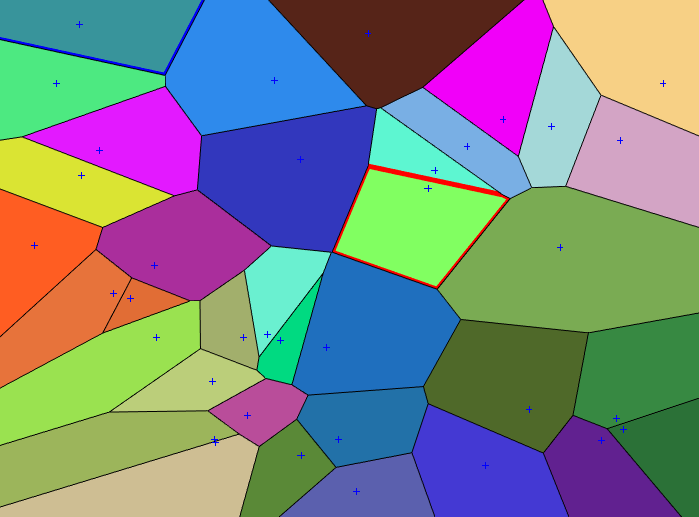
\includegraphics[width=\textwidth]{PCAInterfaceHistEqAfter.png}
		\caption{PCA + Histogram equalisation}
		\label{fig:histEqAfter}
	\end{subfigure}
	\caption{Selection Interface before and after Histogram Equalisation}\label{fig:PCAhistEq}
\end{figure}

Histogram equalisation in one dimension (Fig. \ref{fig:HistEq}) is described below.
\begin{figure}[h] 
	\vspace{-20pt}
	\centering
	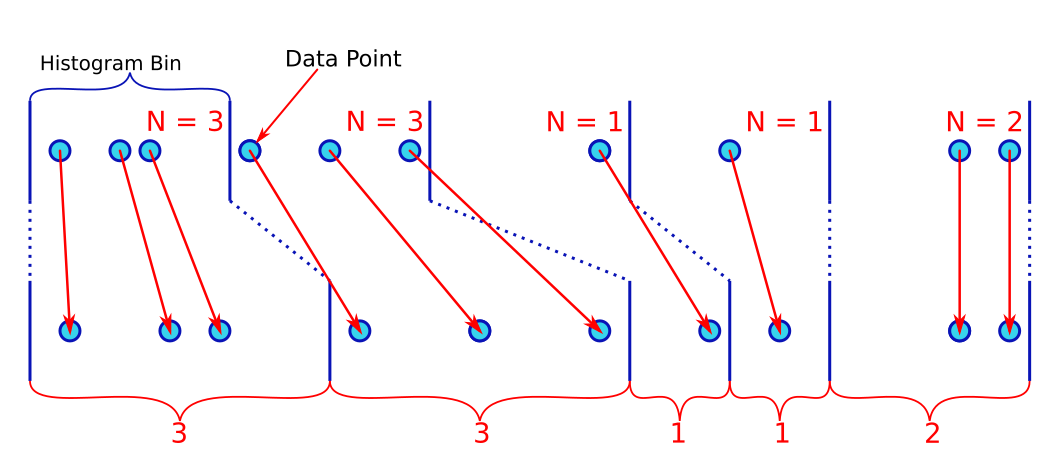
\includegraphics[trim={0, 5pt, 0, 5pt}, clip, width = 6in]{HistogramEquilisation.png}
	\caption{Histogram Equalisation in one dimension}
	\label{fig:HistEq}
\end{figure}\\
A histogram is created by splitting the data into a number of eqully spaced bins (six bins was found to work well for our dataset). The bins are then rescaled, such that the bin width is equal to the number of data points in the bin.

This process is carried out for the presets in all five of the XY-RGB dimensions, and then each dimension is mapped to the range $[-0.95, 0.95]$, such that it will fit inside the axes of $[-1, 1]$. Figures \ref{fig:PCAnumPresets} and \ref{fig:PCAnumPresets2}, show this technique applied to the first three principal components.

This approach, although simple, effectively redistributes the presets. As long as none of the bins are empty, the mapping in each dimension is peicewise-linear and continuous. This means that the Combined Preset Markers can be positioned correctly on the graph by first calculating the PCA scores, then passing these scores through the mapping function. Due to the continuity of the mapping function, the Macro Controls will cause the preset markers to move smoothly across the graph.
\subsection{Demonstrations of Preset Group Clustering}
Having divided the presets into a set of (non-exlusive) categories, the clustering nature of the PCA process can be tested by viewing where the categories are placed in the diagram (Fig. \ref{fig:Categories}). This demonstrates that \textbf{PCA clusters the categories together}, although some are better clustered than others. Part of this is due to the fact that the categories are somewhat subjective, for example the decision between Synth Lead and Synth Pad, or between Piano/Keys and Plucked/Mallet. Some of the categories also include a wide range of sounds, especially Rhythmic and Synth Lead, and so have a less consistent pattern in their parameters.\\
Key limitations of the above analysis are the small sample size of presets, and the fact that many of the presets were made by using the Blending Interface, so potentially have overly similar parameters than if they'd been made from scratch by a person. To validate this approach more thoroughly, sets of presets from several pre-existing commercial synths should be tested. Once this larger dataset has been collected, a comparision of different dimensionality reduction techniques should be carried out.

\begin{figure}
	\centering
	\begin{subfigure}[b]{0.48\textwidth}
		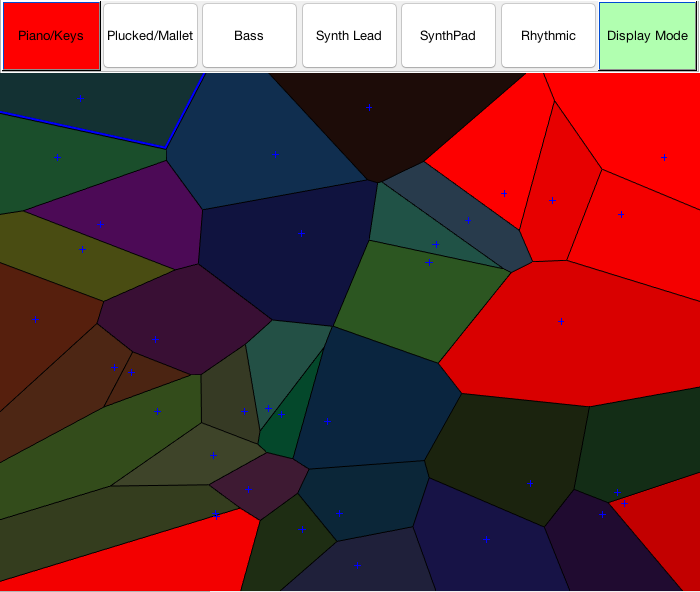
\includegraphics[width=\textwidth]{CategoryPianoKeys.png}
		\caption{Piano/Keys}
		\label{fig:categoriesPianoKeys}
	\end{subfigure}
	~ %add desired spacing between images, e. g. ~, \quad, \qquad, \hfill etc. 
	%(or a blank line to force the subfigure onto a new line)
	\begin{subfigure}[b]{0.48\textwidth}
		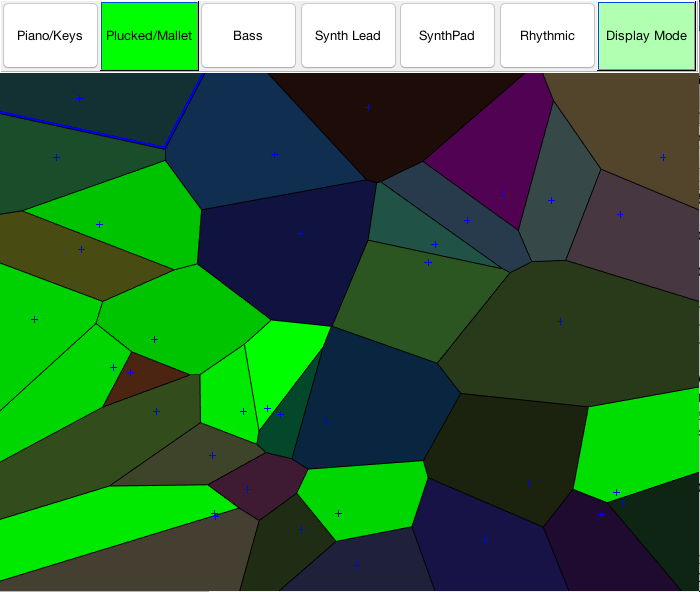
\includegraphics[trim={0 0 0.01cm 0}, clip, width=\textwidth]{CategoryPluckedMallet.png}
		\caption{Plucked/Mallet}
		\label{fig:categoriesPluckedMallet}
	\end{subfigure}
\\ 
\begin{subfigure}[b]{0.48\textwidth}
	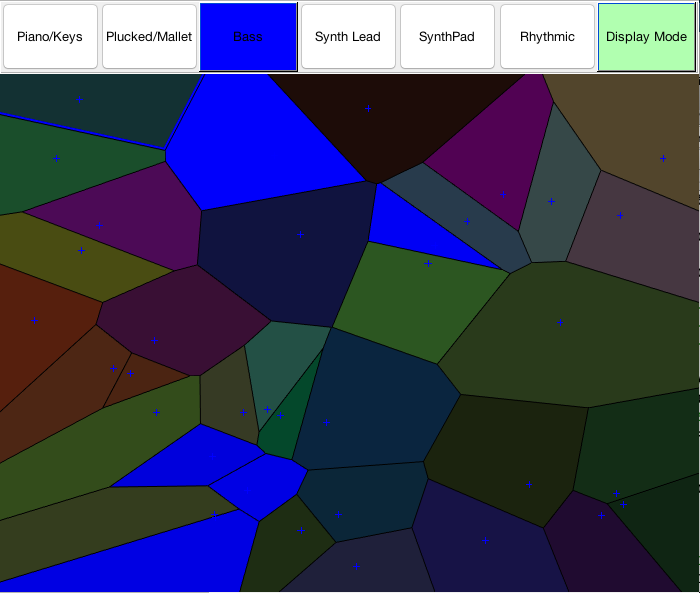
\includegraphics[width=\textwidth]{CategoryBass.png}
	\caption{Bass}
	\label{fig:categoriesBass}
\end{subfigure}
~ %add desired spacing between images, e. g. ~, \quad, \qquad, \hfill etc. 
%(or a blank line to force the subfigure onto a new line)
\begin{subfigure}[b]{0.48\textwidth}
	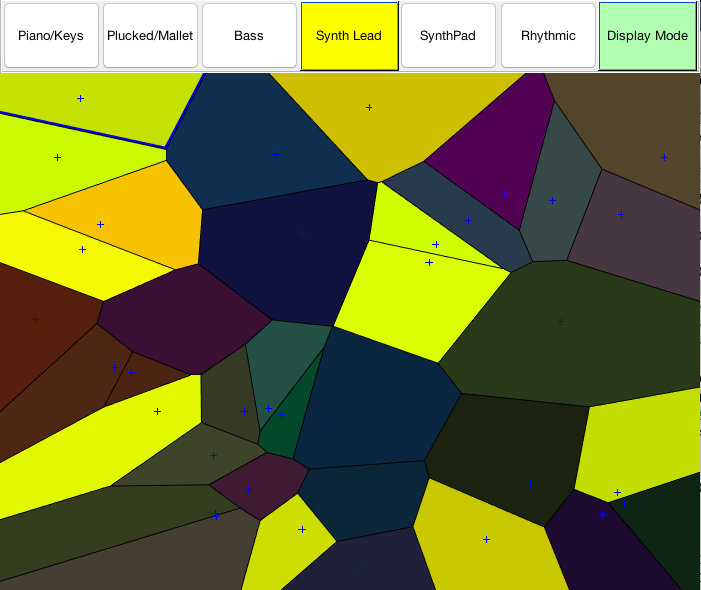
\includegraphics[trim={0 0 0.01cm 0}, clip, width=\textwidth]{CategorySynthLead.png}
	\caption{Synth Lead}
	\label{fig:categoriesSynthLead}
\end{subfigure}
\\
\begin{subfigure}[b]{0.48\textwidth}
	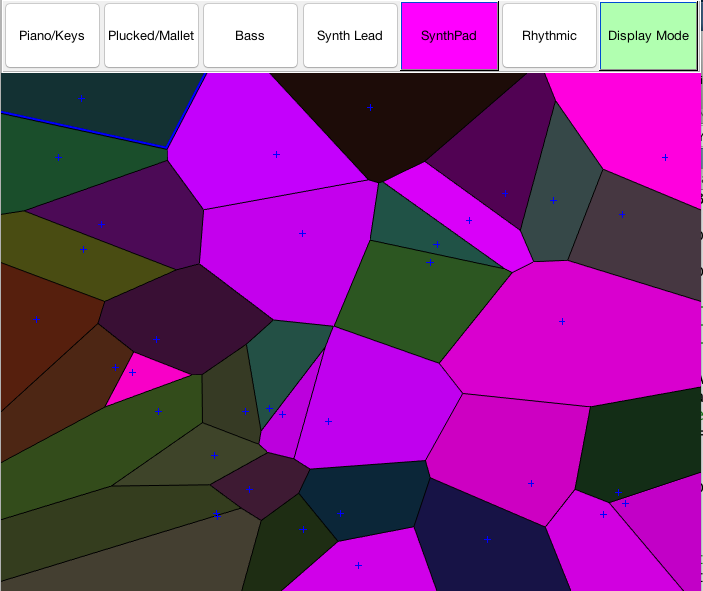
\includegraphics[trim={0 0 0.01cm 0}, clip, width=\textwidth]{CategorySynthPad.png}
	\caption{Synth Pad}
	\label{fig:categoriesSynthPad}
\end{subfigure}
~ %add desired spacing between images, e. g. ~, \quad, \qquad, \hfill etc. 
%(or a blank line to force the subfigure onto a new line)
\begin{subfigure}[b]{0.48\textwidth}
	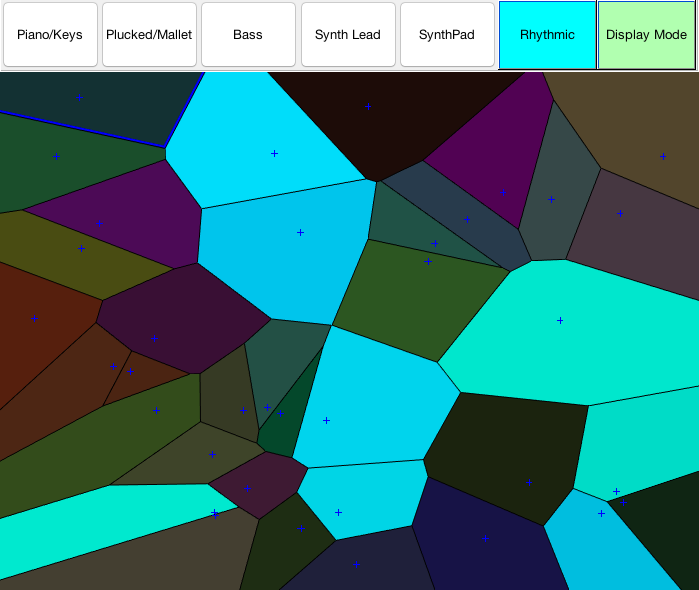
\includegraphics[width=\textwidth]{CategoryRhythmic.png}
	\caption{Rhythmic}
	\label{fig:categoriesRhythmic}
\end{subfigure}
	\caption{Preset Categories shown on Selection Interface - For ceratin categories, such as Piano/Keys and Plucked/Mallet, the PCA + Histogram Equalisation mapping has effectively clustered the presets together. Other categories, such as Synth Lead, are less clustered.}
	\label{fig:Categories}
\end{figure}

\subsection{How the PCA Mapping Scales with Number of Presets}
The consistency of the PCA mapping as more presets are added is of importance to the usefulness of the interface. If the mapping radically changes every time a new preset is added, then any intuitition the user has learned about what the different components represent will be lost. This is one of the reasons for choosing PCA, as the linearity of the technique should lead to less surprising results than stochastic, non-linear techniques such as \emph{tSNE}.\\
\begin{figure}[h]
	\hspace{-80pt}
	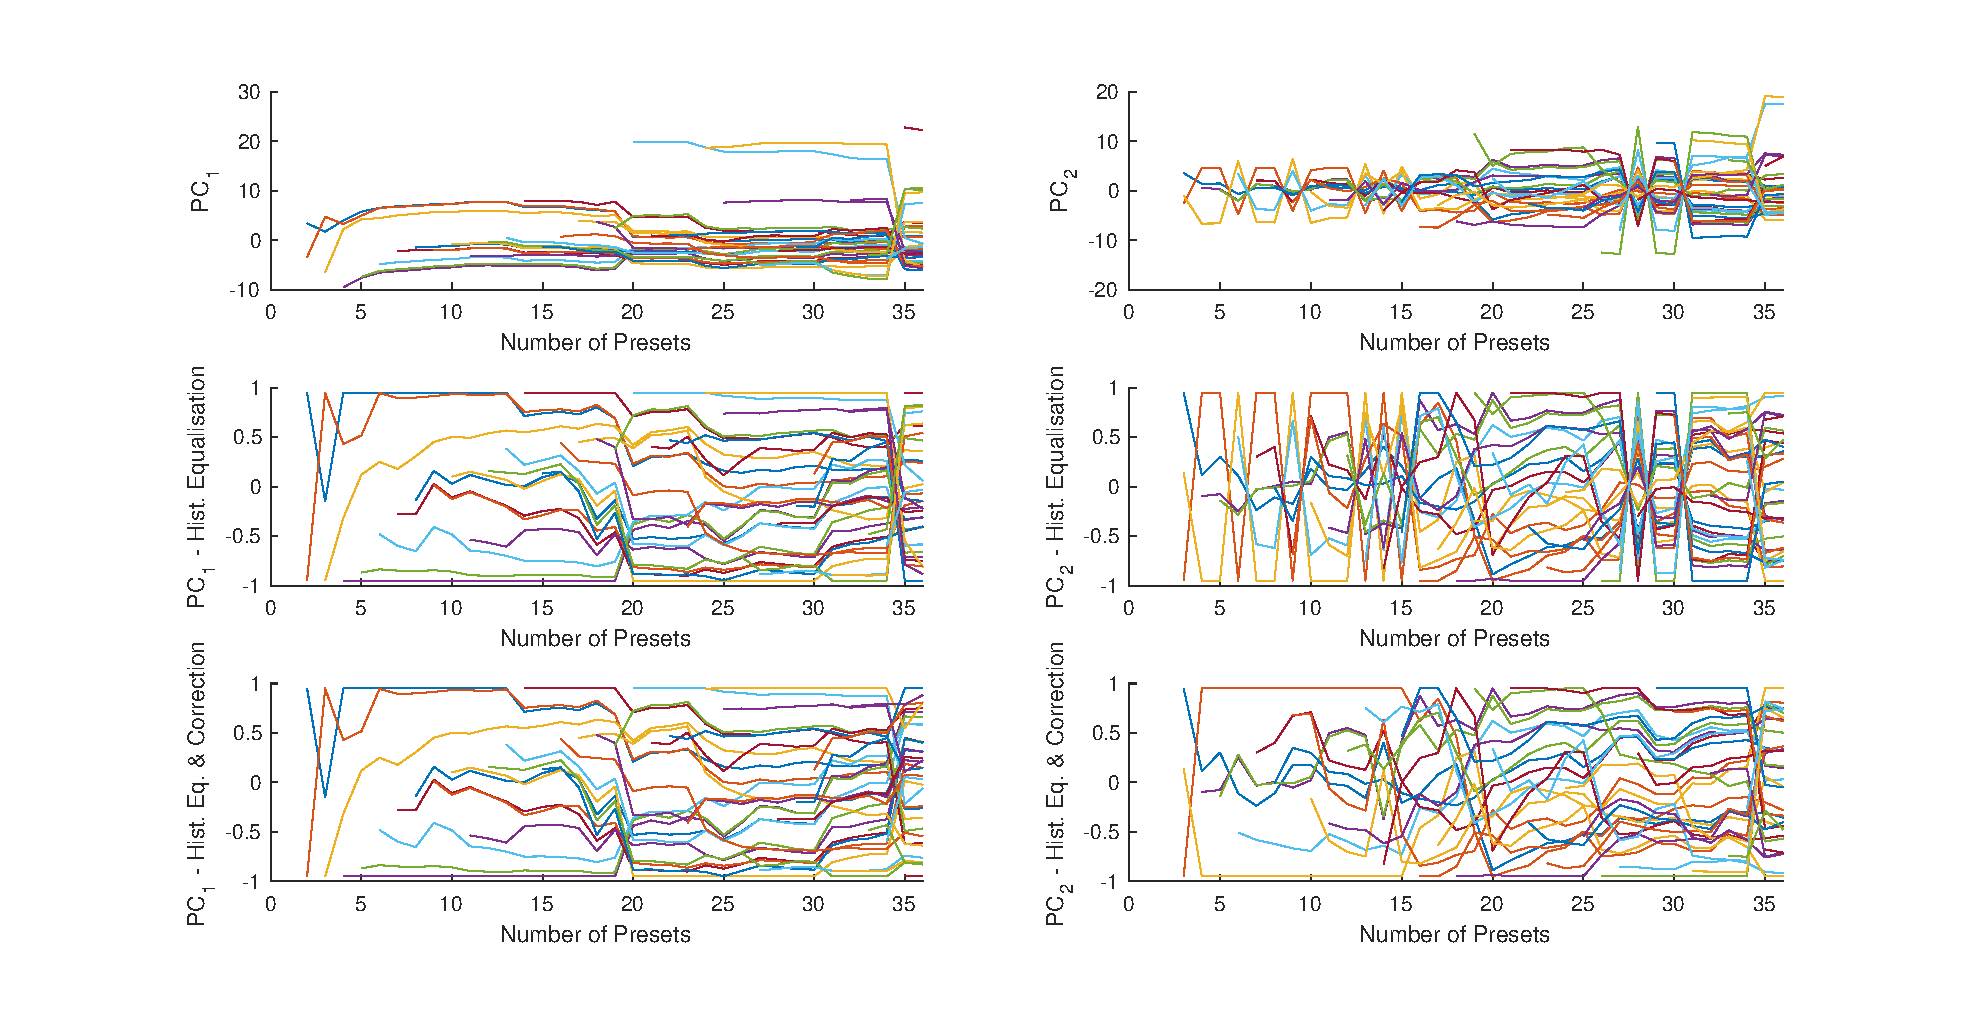
\includegraphics[trim={0, 1cm, 0, 1cm}, clip, width = 8.5in]{PCAnumPresets1.eps}
	\caption{PCA stability with number of presets. These plots show the positions of the indiviual presets when mapped onto the first and second principal components, with and without Histogram Equalisation. The mapping is recalculated each time a new preset is added. The positions are relatively stable except at discrete points where the component flips. These flips can be automatically corrected, as shown in the thrid row, with details of the correction process shown in Fig. \ref{fig:PCAnumPresets2}.}
	\label{fig:PCAnumPresets}
		\vspace{-10pt}
\end{figure}
Fig. \ref{fig:PCAnumPresets} shows the variation of the preset positions for the first two principal components as the presets are added one at a time in the order of creation. After Histogram Equalisation has been applied the components are relatively stable, except at certain points where the component flips sign. This can be seen at preset 34 for $PC_1$, and presets 6, 9, 13, 15, 28, 31:36 for $PC_2$. The bottom row of the figure shows the components after this sign flipping has been corrected. This makes a dramatic improvement in the stability of the mapping, especially for $PC_2$. This phenomenon also occurs in $PC_{3,4,5}$ used for the RGB mapping of the presets.

As PCA is very quick to compute, the necessary sign reversals to correct the components can easily be computed using dynamic programming.\\ Defining $PCA_i^k$ to be the $i$th principal component computed with $k$ presets.
\begin{itemize}
%	\vspace{-10pt}
		\setlength\itemsep{-1.2em}
	\item 
Iterate from $k = 1$, to $k = N-1$, where $N$ is the number of presets.
	\item 
If $\|PCA_i^{k+1} - PCA_i^k)\|_1 > \|PCA_i^{k+1} - (-PCA_i^k))\|_1$,  flip the sign of all remaining presets.
%\vspace{-30pt}
\end{itemize}
This algorithm is used on $PC_3$ in Fig. \ref{fig:PCAnumPresets2}. In order for this algorithm to work well, the preset mapping needs to be Histogram Normalised and centered on zero. To implement the algorithm in the interface, all that it necessary to do is keep track of which components have been flipped, and each time a new preset is added, check if $\|PCA_i^{k+1} - PCA_i^k)\|_1 > \|PCA_i^{k+1} - (-PCA_i^k))\|_1$ to determine whether to flip component $i$, and update the record of flipped components. 

\begin{figure}
	\hspace{-40pt}
	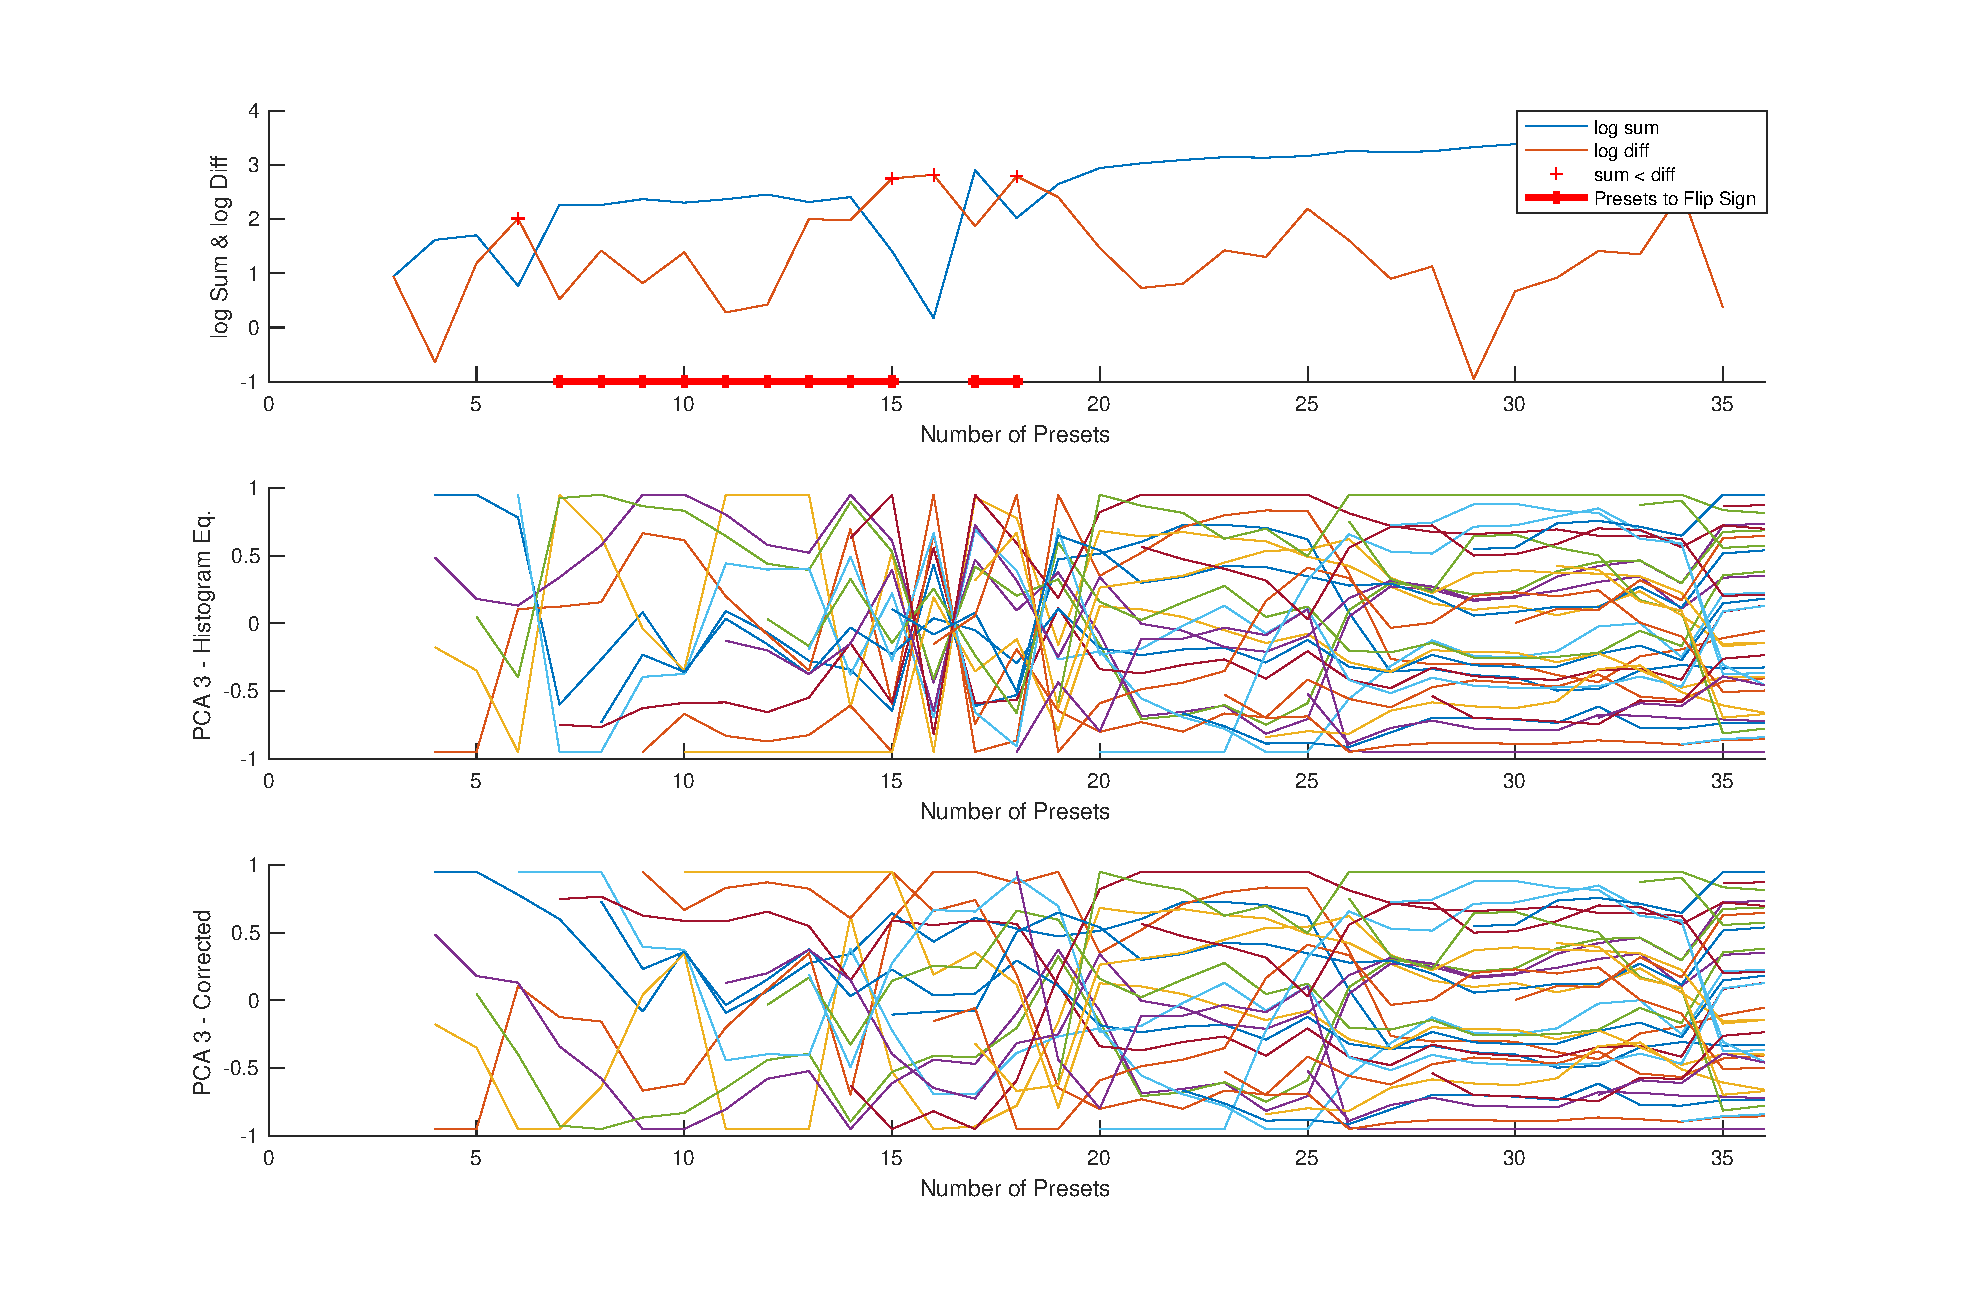
\includegraphics[trim={0, 1cm, 0, 1.5cm}, clip, width = 7in]{PCAnumPresets2.eps}
	\caption{PCA Sign Flip Correction Algorithm.}
	\label{fig:PCAnumPresets2}
	\vspace{-10pt}
\end{figure}

The variance of each principal component can be used to measure the effectiveness of the PCA mapping. If the first few components account for most of the variance of the dataset, then the dimensionality reduction has been successful.
Fig. \ref{fig:LatentOriginal} shows how the fraction of the variance associated with each principal component changes as more presets are added. Over 50\% of the variance can be accounted for by $PC_{1,2}$,  over 90\% by $PC_{1 : 10}$, and the graph assymtotes to a relatively stable state. Fig. \ref{fig:LatentRandom} is the same plot for a random dataset the same size as the original dataset. Each of the fractions is rougly exponentially decreasing. When all 36 presets are included, only 50\% of the variance can be accounted for by $PC_{1 : 10}$. \\
It appears that synth dataset has some non-random internal structure which PCA is successfully managing to find. This suggests that \textbf{PCA is an appropriate technique to use on synth datasets}, however testing on other synth datasets is necessary to validate this result.
\begin{figure}[h]
	\vspace{-5pt}
	\hspace{-40pt}
	\begin{subfigure}{3.5in}
		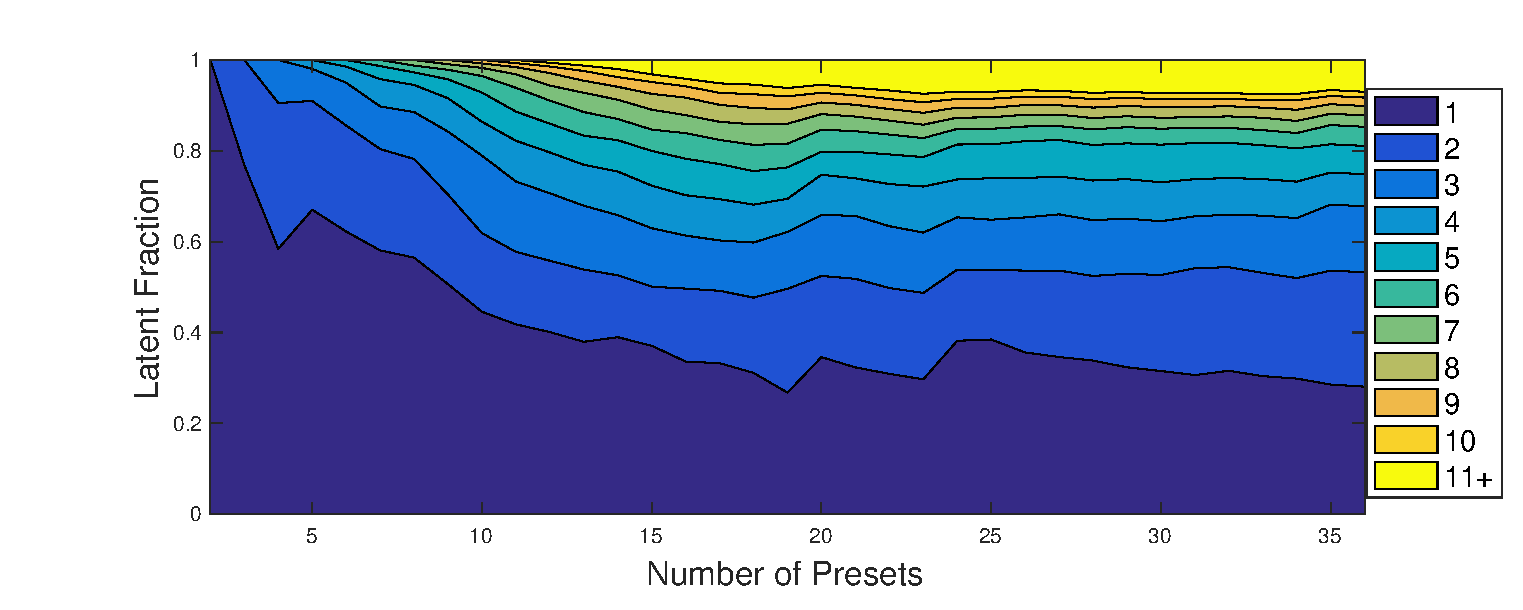
\includegraphics[trim = {0, 0.1cm, 0, 0.5cm}, clip, width = \textwidth]{LatentFraction.eps}
		\caption{Original Presets}
		\label{fig:LatentOriginal}
	\end{subfigure} 
%
	\begin{subfigure}{3.5in}
		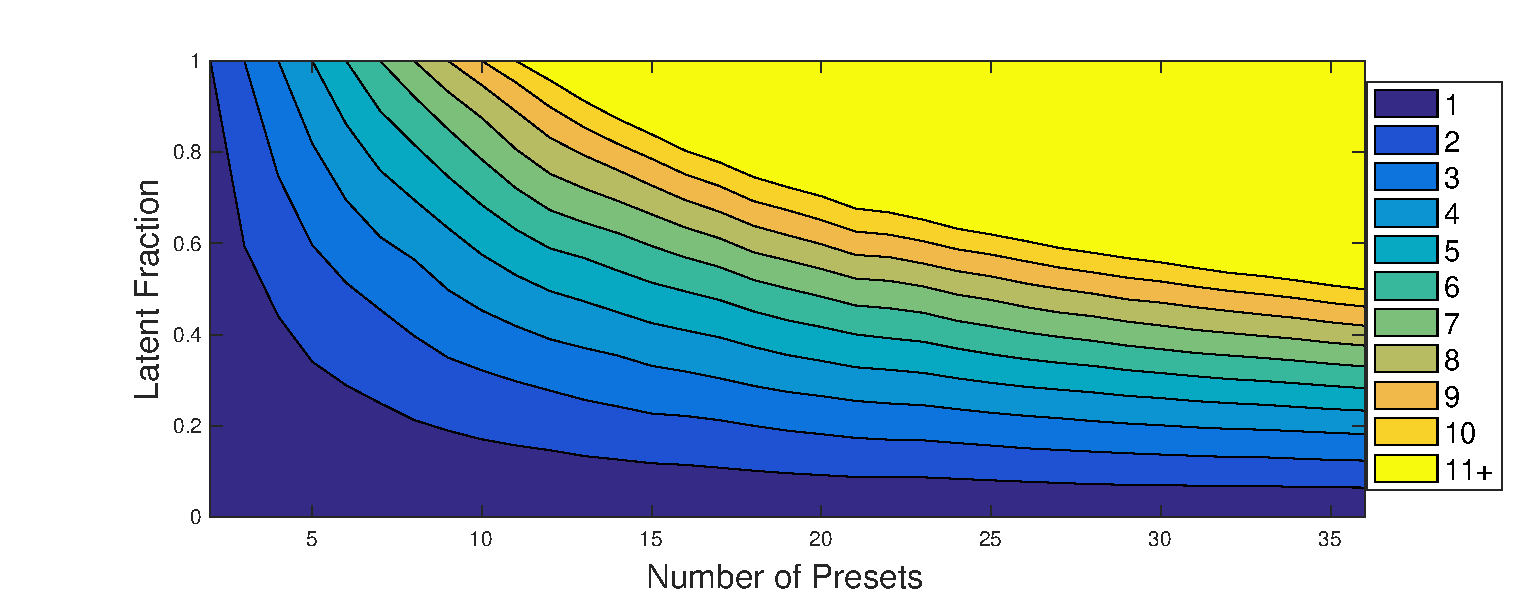
\includegraphics[trim = {0, 0.1cm, 0, 0.5cm}, clip, width = \textwidth]{LatentFractionRandom.eps}
		\caption{Randomised Presets}
		\label{fig:LatentRandom}
	\end{subfigure}
	\caption{Variance Fraction - Colour denotes Principal Component number}
	%	\vspace{-30pt}
\end{figure}


%\subsection{Quantify the extra variance the macro controls give}
%asdasdasdsa
%\subsection{Investigate Permutation Ambiguity}
%asdasdsa

\pagebreak
\section{Blending Interface}
\subsection{Detailed Description}\label{sec:BlendingDescription}
This interface was created as a Matlab figure-based application. Fig. \ref{fig:BlendingAlgorithm} shows the the key steps of the Blending Interface's algorithm.

\begin{figure}[h] 
	\centering
	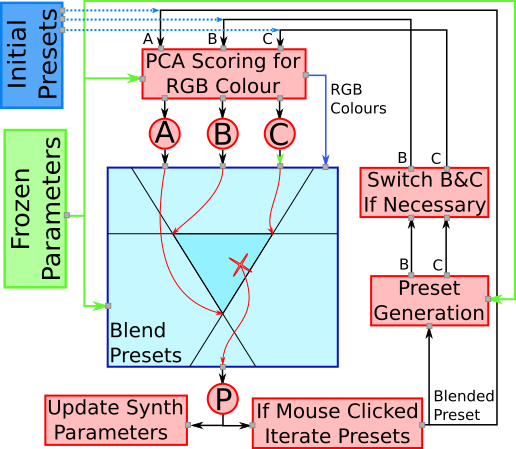
\includegraphics[width = 5in]{BlendingAlgorithm.png}
	\caption{Blending Algorithm flow chart}
	\label{fig:BlendingAlgorithm}
\end{figure}
%
The blending of presets is calculated as a non orthogonal vetor decomposition: \cite{NonOrthogonal}
\begin{equation}
	\vec{P} = f(\alpha\vec{A} + \beta\vec{B} + \gamma\vec{C})
	\label{eq:PresetMix}
\end{equation}
Where $\vec{P}$ is the blended preset, $\vec{A}$, $\vec{B}$, $\vec{C}$ are presets A, B and C, $f$ is a function which applies parameter constraints, and $\alpha$, $\beta$ and $\gamma$ are calculated from the following matrix equation:
\begin{equation}
[\beta,  \gamma]^T = (\vec{M}^T\vec{M})\vec{M}^T[x, y], 
	\hspace{1in} \alpha = 1 - (\beta + \gamma)
\end{equation}
\begin{wrapfigure}{R}{0.35\textwidth}
	\vspace{-10pt}
	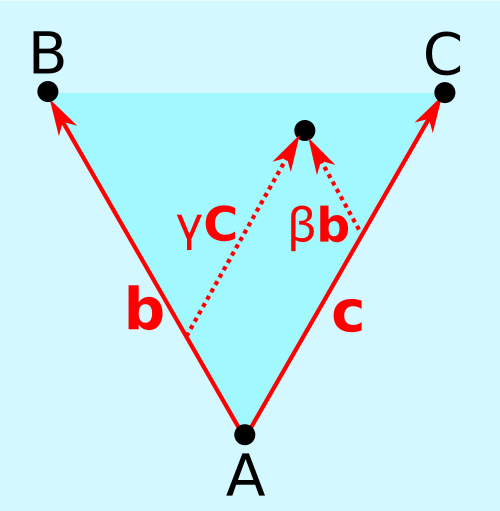
\includegraphics[width = \textwidth/3]{BlendVectors.png}
	\caption{Non-orthogonal vector decomposition}
	\label{fig:BlendingVectors}
	%\vspace{-60pt}
	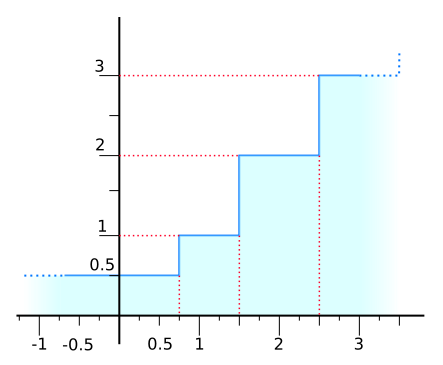
\includegraphics[width = \textwidth/3]{FreqCoarse.png}
	\caption{Mapping from continuous to coarse frequency}
	\label{fig:Freq Coarse}
	%\vspace{-60pt}
	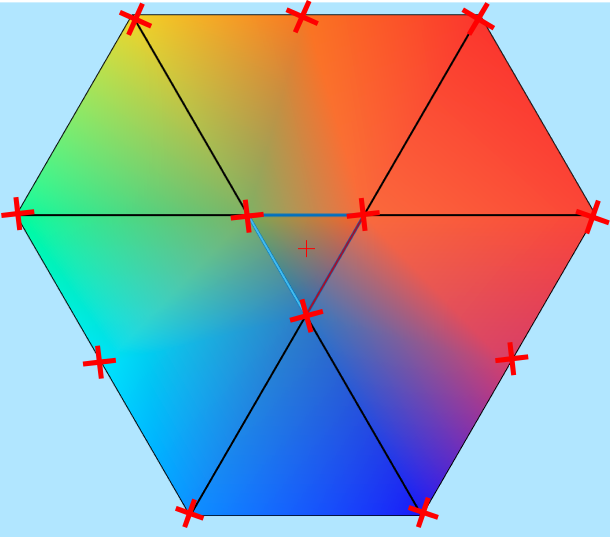
\includegraphics[width = \textwidth/3]{BlendingColours2.png}
	\caption{$PC_{3,4,5}$ applied to RGB colour of Blending Interface}
	\label{fig:BlendingColours}
	\vspace{-30pt}
\end{wrapfigure}
where $x$ and $y$ are the x and y coordinates of the current cursor position, and $\vec{M} =[\vec{b},  \vec{c}]$, where $\vec{b}$,  $\vec{c}$ are vectors from preset location A to the B and C locations (Fig. \ref{fig:BlendingVectors}). There are two reasons for blending the presets in this way. Firstly, on an $m$-dimensional control surface, it is possible to linearly interpolate between all possible combinations of $m+1$ presets, so on a 2D screen, three presets should be used.\footnote{Some implementations of preset blending in commercial synthesisers use four presets located on the corners of a square, however in this arrangement it is not possible to reach all possible combinations.} Secondly, this arrangment allows for locations both inside and outside of the central triangle to be used. Inside the triangle, $\alpha$, $\beta$ and $\gamma$ are all in the range [0, 1], giving an \emph{interpolation} between the presets. Outside of the triangle $\alpha$, $\beta$ and $\gamma$ can be less than zero and greater than one, allowing for \emph{extrapolation}.

The parameter constraint function, $f$, applies the relevant constraints to each parameter. Most parameters are continuous with an upper and lower bound, $[l, u]$. For these parameters: $f_i(P_i) = \min(\max(P_i, l), u)$, where $P_i$ is the $i$th parameter of blended preset $\vec{P}$. For the Coarse Frequency parameters, the continuous blended value is discretised to the set $\{0.5, 1, 2, 3, ...\}$, with the desicion boundary equidistant from neighbouring numbers (Fig. \ref{fig:Freq Coarse}).

To make the iterative blending process more intuitive, and to maintain consistency between the interfaces, the PCA based RGB colouring from the Selection Interface was used. Equation \ref{eq:PresetMix} is used to calculate the blended preset at each of the points marked on Fig. \ref{fig:BlendingColours}, and the PCA Scores are evaluated for each point. $PC_{3,4,5}$ are mapped to RGB colour, and colour is linearly interpolated between the points. A more detailed colour space can be acheived by using more points, but there is an associated performance tradeoff. 

\begin{wrapfigure}{R}{0.3\textwidth}
	\centering
	%\vspace{-40pt}
	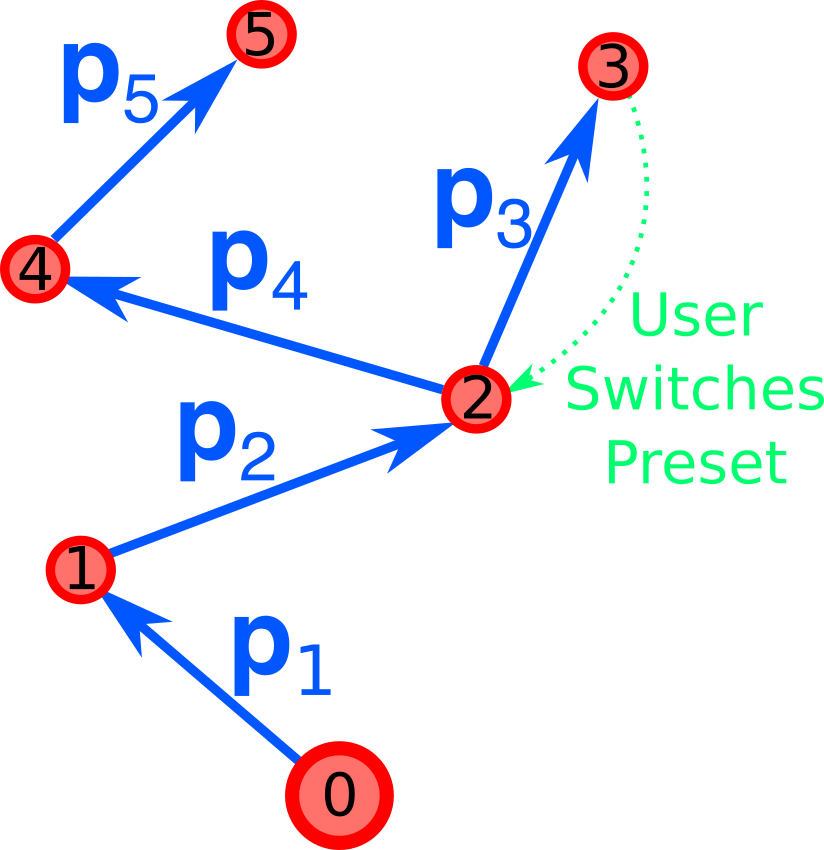
\includegraphics[width = \textwidth/3]{SelectionHistory.png}
	\caption{Selection History plot construction}
	\label{fig:SelectionHistory}
	\vspace{7pt}
	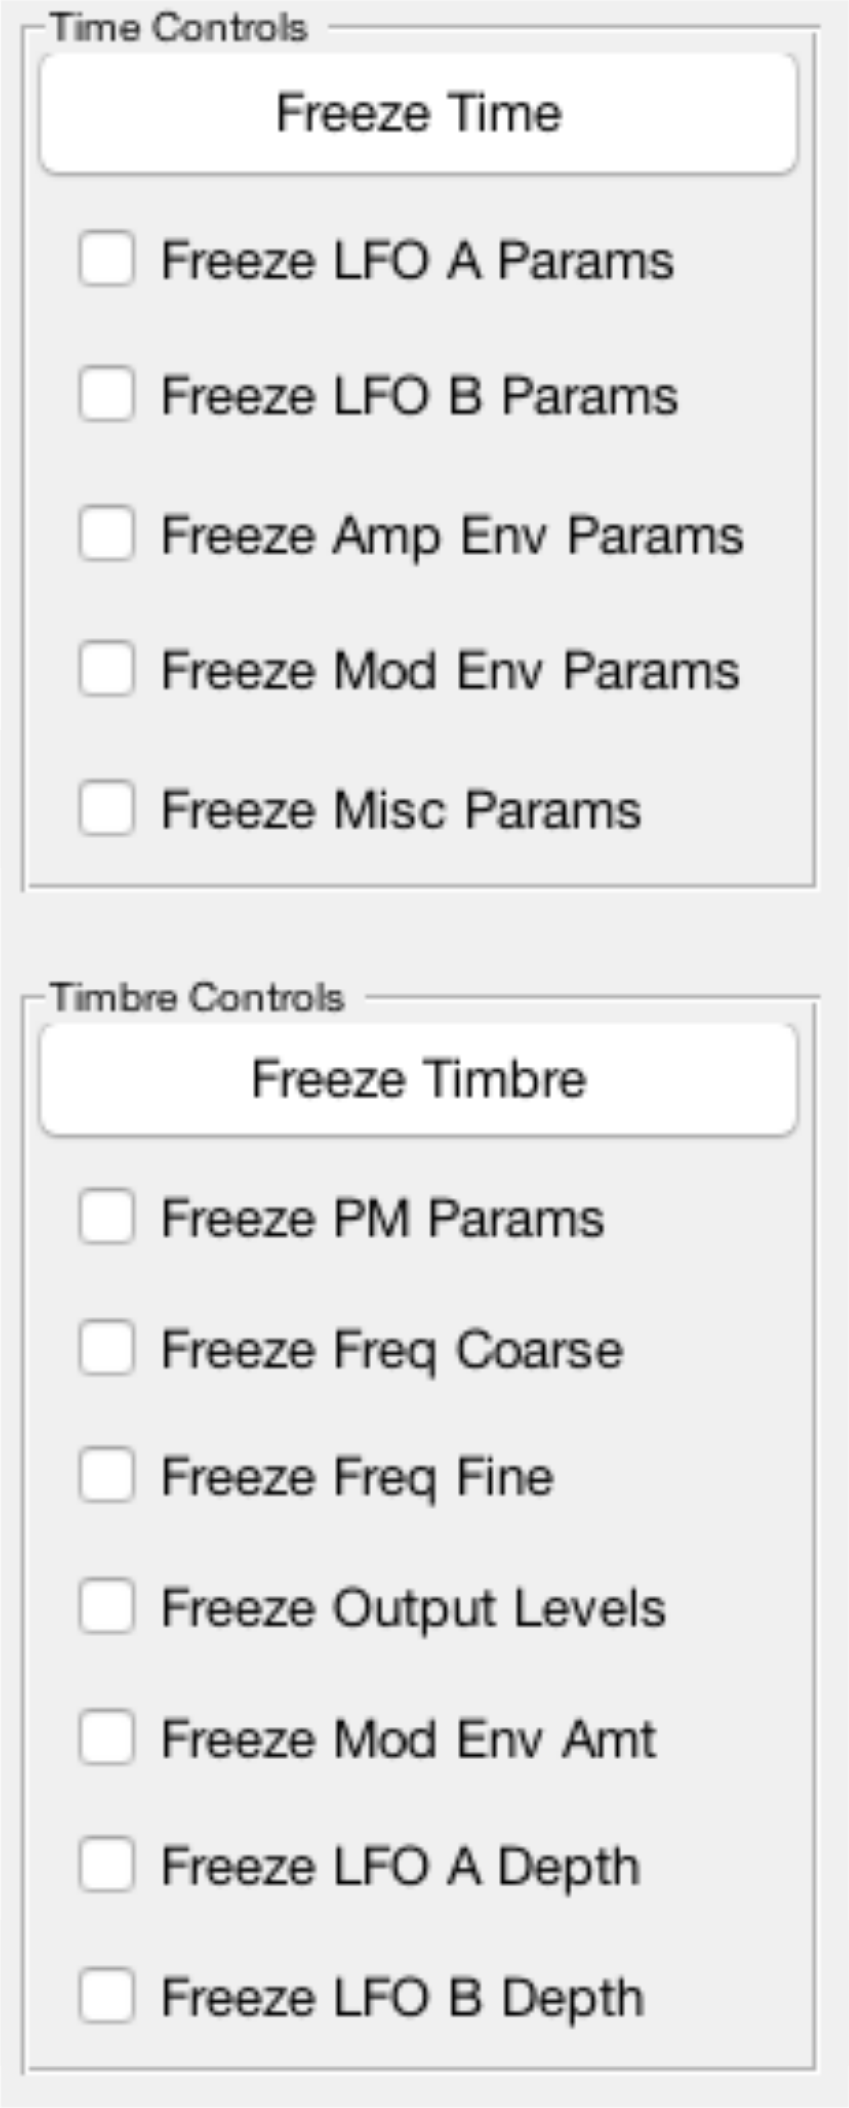
\includegraphics[width = \textwidth/3]{FreezeParams2.png}
	\caption{Parameter Freezing}
	\label{fig:FreezeParams}
	\vspace{-70pt}
\end{wrapfigure}

Each time the presets are iterated, the first principal component, $PC_{1}$ is calculated for the generated presets B and C. If $PC_{1}^B > PC_{1}^C $, then presets B and C are swapped. This makes the $x$ direction in the Blending Interface correspond to a direction of increasing $PC_{1}$. This is done to maintain consistency between the two interfaces, as $PC_{1}$ is also used in the Selection Interface for the $x$ coordinate of each preset.

The Selection History display allows the user to browse their previously selected presets, by clicking on nodes of the graph. Each time presets are iterated, the vector from A to the selelected coordinates, $\vec{p}_i$ is recorded. The graph is constucted by joining these vectors head-to-tail (Fig. \ref{fig:SelectionHistory}). The colours of each edge of the graph are chosen based on $PC_{3,4,5}$ of the presets. See Fig. \ref{fig:BlendingInterface} for a typical  Selection History plot.

It may be possible to use some of the information contained in the graph (if the data from many users is collected), as a way to refine the preset generation algorithm. If the generation algorithm is producing good presets, then most of the choices should be somewhere between A, B and C on the interface. If the algorithm is producing bad presets, most of the choices will be very close to, or below A.

The user has the option to freeze sections of the parameter space (Fig. \ref{fig:FreezeParams}). The parameters are divided into Time and Timbre parameters, and then subdivided into a total of 12 smaller categories (Table \ref{tab:Params}). This makes the Blending Interface more useful, as it allows users with knowledge of synthesisers to fine-tune the blending process to their needs. This tends to lead to more useful generated presets, as it reduces the dimensionality of the search space.

\subsection{Preset Generation Algorithm} \label{sec:PresetGeneration}
The aim of the Preset Generation Algorithm is to suggest useful new presets, based on the user's previous selections. In the field of \emph{Active Learning} \cite{ActiveLearning}, several similar problems have been adressed, the most relevant of which is a preference-gallery based approach to fine-tuning parametric procedural animations \cite{PreferenceGallery}.
In this work a user is iteratively presented with a four generated aminations, and selects their favourite. In each iteration, \emph{Bayesian optimisation} is used to learn from the previous selections, and generate four new animations. This procedure was shown to be superior to both a slider-based interface, and an interface in which the user rates each animation on a numeric scale. The gallery interface was improved by allowing the user to manually set and freeze parameters, especially for expert-users. Bayesian optimisation is well suited to this task, as it explicitely deals with the \emph{exploration-exploitation} tradeoff \cite{ExplorationExploitation} and is designed to minimise the number of user queries. However, the main limitation with this work is that traditional Bayesian Optimisation can only be used for problems with low ($<20$) dimensionality due to an the exponential increase in necessary user queries. The animation model only had 12 parameters, and this still took a considerable ammount of training data to fine-tune the hyperparameters of the learning algorithm.  Adaptations of bayesian optimisation have managed to solve certain higher-dimensional problems \cite{BayesOptDimensionality}, but it is currently non-trivial to apply these results to general problems. Therefore an alternative algorithm was developed.

The new presets are a weighted sum of the previously selected presets, with gaussian noise added.
Let $\vec{H} = [\vec{h}_1, \vec{h}_2, \dots \vec{h}_m]^T$ where $\vec{h}_i$ is the $i$th previously selected preset.
Let $w = \frac{1}{1 + exp(-a*(x-c))}$

\begin{figure}
	\centering
	%\vspace{-110pt}
	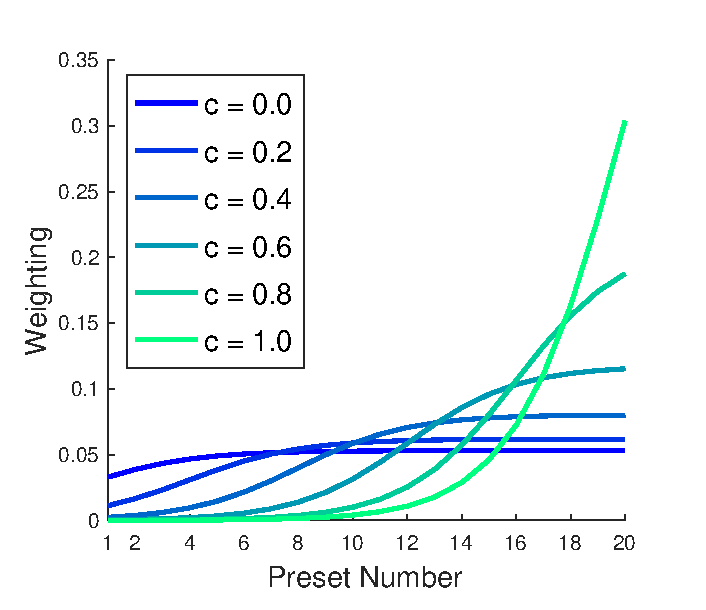
\includegraphics[width = 3.1in]{SigmoidWeights.eps}
	\caption{Sigmoid weighting function}
	\label{fig:SigmoidWeights}
	
	%	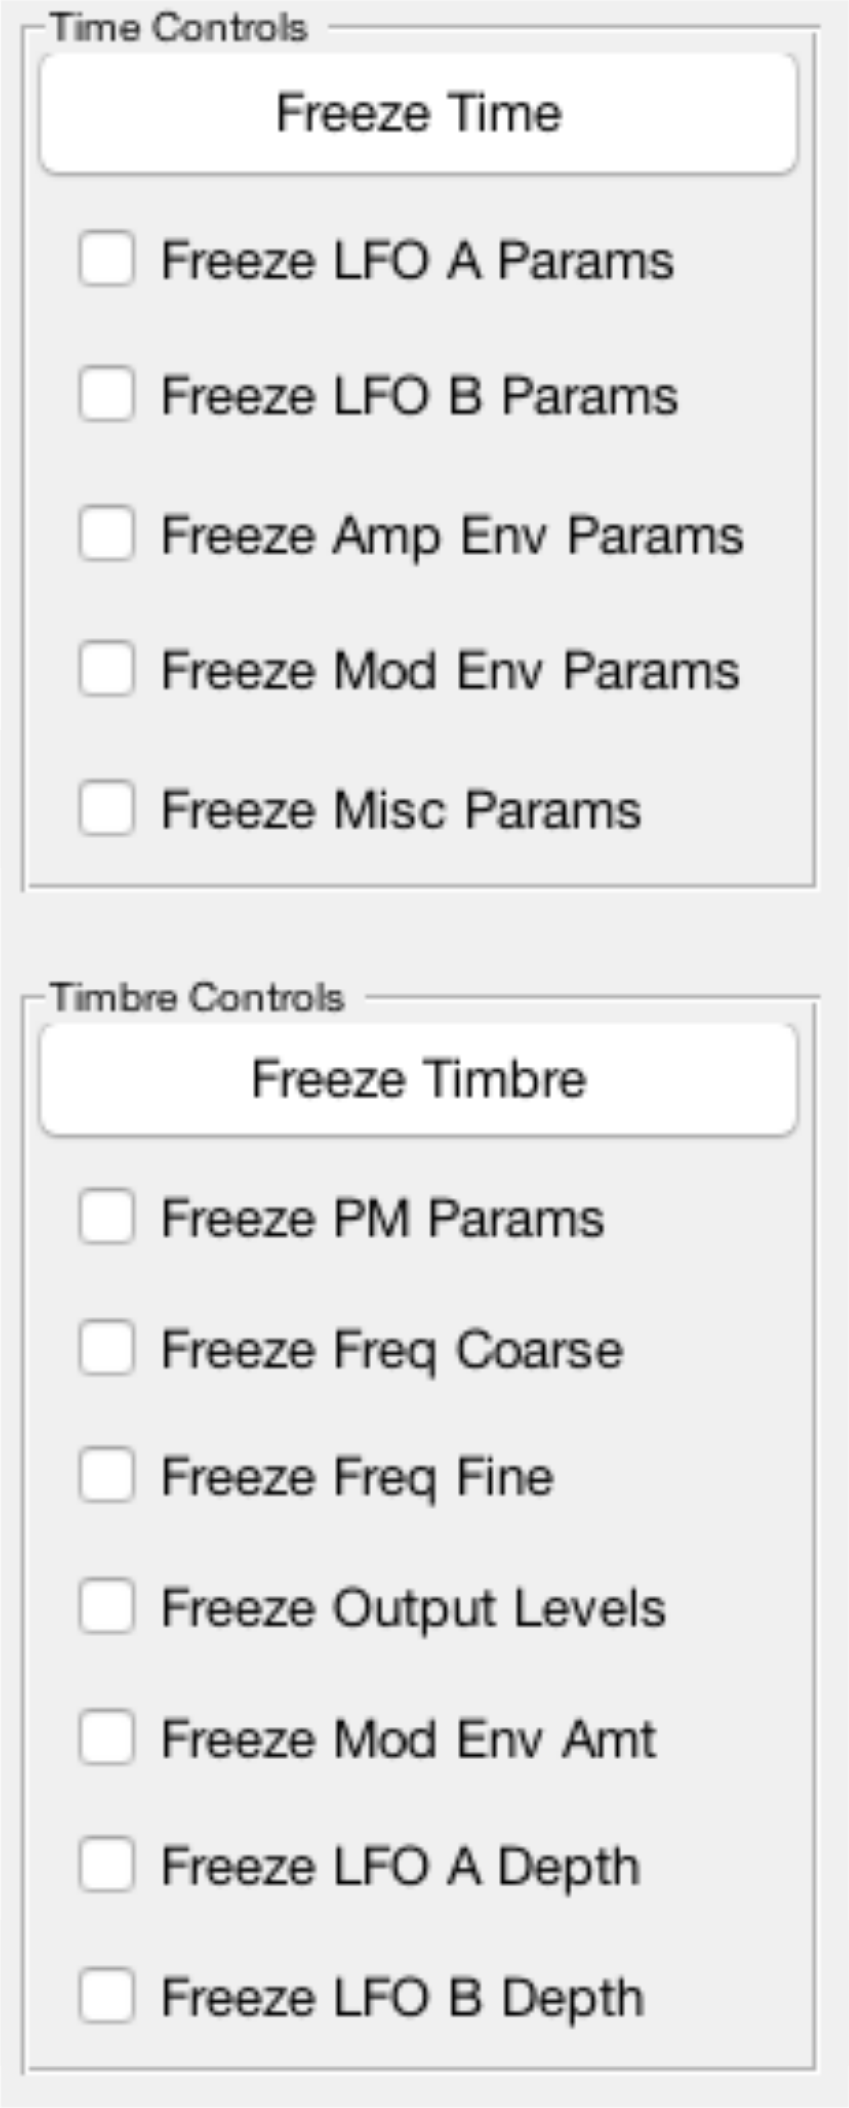
\includegraphics[width = \textwidth/3]{FreezeParams2.png}
	%	\caption{Parameter Freezing}
	%	\label{fig:FreezeParams}
	
	%\vspace{-60pt}
	
\end{figure}
\section{Investigion of Permutation Ambiguity}\label{sec:PermutationAmbiguity}
Due to the equivilance of the six operators of the synth architecture, there is the possibility of permutation ambiguity in the dataset (\S \ref{sec:SynthDescription}). However it may be possible to correct for this using knowledge of the synth architecture. Typically the operators with the loudest Output Level parameters act as \emph{modulators} and the operators with lower output levels act as \emph{carriers} (as defined in \cite{YeeKing}, Section 3.1.1). Therefore the dataset can be permutation-alligned by permuting each preset, such that the Output Level parameters are in decreasing order.\\
To determine the sucess of this approach, the original dataset was compared to the permuted dataset, and a randomly permuted dataset , using the following cost function:
\begin{equation}
	C = \sum_{i = 1}^{N}\sum_{j = i+1}^{N}\mathrm{error}(\vec{P}_i, \vec{P}_j)
\end{equation}
where $N$ is the number of presets, and $\mathrm{error}$ is the error metric defined in Section \ref{sec:ErrorMetric} with only the Timbre parameters included (As only these exhibit permutation ambiguity).\\
The results of this evaluluation is shown in Table \ref{tab:PermutationAmbiguity}. The permutation-alligned dataset has a similar cost to the original dataset, and a 15\% lower cost than the randomly permuted data. It is worth noting that when creating the original dataset, most presets were designed to minimise permutation ambiguity, and so exhibit lower levels than a typical synth preset dataset might.  The interface was tested after permutation-alligning the presets, which seemed to improve the usefulness of the Macro Controls, and made the Blending Interface create more useful sounds. Furthermore the category clustering perfomance wasn't degraded. Based on the results, permutation-allignment seems to be a worthwhile endevour, as it gives a sigificant improvement over randomly permutated dataset, and gives potential improvements to the usefulness of the interface. More work needs to be done to thoroughly evaluate this technique, and to determine if incorporating more knowledge of the synth architecture can make the process more effective.
\begin{table}[h]
	\centering
	\begin{tabular}{l|l|l|l}
		& Original Dataset & Permutation-Alligned & Randomly Permuted \\ \hline
		Cost $\times 10^4$ & 2.427            & 2.452                 & 2.8264  (mean of 50 runs, $\sigma = 0.0098$)
	\end{tabular}
\caption{Permutation Ambiguity Evaluation Results}
\label{tab:PermutationAmbiguity}
\end{table}


\chapter{Numerical Evaluation of Interfaces}
Due to the subjectivity of interface design, and as the three interfaces have quite different purposes, there are not many obvious metrics to use to compare the interfaces with each other. However, the key challenge is to make the combined interface better than the traditional interface alone. MORE WRITING - PRIOR WORK? MEASURE OF REGRET>?
\section{Perfect/Imperfect User Model}
A way of evaluating the performance of the interface is to simulate a Perfect User, and an Imperfect User carying out a range of tasks. These simulated users must use the interface to move from initial presets to goal presets. This analysis won't account for any creativity based goals of the interface, but will help evaluate some of the practical considerations of the interface. (BAD WORDING< WORK ON THIS SECTION).
 
The Perfect User has perfect knowledge of the synth and the interface, so can always choose the optimum position for a particular knob, or choose the optimum blend of presets in the Blending Interface.

The Imperfect User has imperfect knowledge of the synth and the interface, so chooses interactions similarly to the Perfect User, but misses by a certain amount: $\Delta P_i = \Delta P_i^0 * (1 + \varepsilon)$, where $\Delta P_i^0$ is the Perfect parameter change, and $\varepsilon$ is a zero-mean Gaussian random variable with variance $\sigma^2$. Various values of $\sigma$ will be considered to account for the varying skill levels of users.

A key consideration for the Traditional Interface is the order which parameters are varied. In the Perfect Order, parameters are visited in decreasing order of importance. In the Random Order, parameters are visited in a completely random order. Real users most likely operate somewhere in the middle of these regimes. (REFERENCE FOR THIS>???)

\section{Error Metric}\label{sec:ErrorMetric}
A parameter-based error metric is used for these tasks due to the complexity of using a sound based comparisons of presets (\S \ref{MachineLearning}).
%COULD USE THE Index of Search Space Reduction (ISSR) Approach from Robert Tubbs thesis.
For each parameter, $p_i$, a weighted $L_1$ norm is used. The parameters are weighted based on an approximate measure of importance, and normalised by their parameter ranges. The total error is calculated as:
\begin{equation}
E = \sum_{i=1}^{N}\frac{w_i}{r_i} \| p_i - p_i^{goal} \|_1 
\end{equation}
where $w_i$ is the scalar importance weighting for the $i$th parameter, and $r_i$ is the range of values that parameter $i$ can take (see Table \ref{tab:Params}).

The $L_1$ norm was chosen over the $L_2$ norm so that a few large parameter errors don't dominate the error metric and as no gradients are necessary.
It may be possible to incorporate more knowledge of the synth into the error metric to explicitely remove the effect of permutation ambiguity, and to better approximate the results of a sound-based error metric. A similar parameter based metric is the \emph{Index of Search Space Reduction} \cite{TubbThesis}.

\section{Comparison of Isolated Interfaces}
\subsection{Traditional Interface}\label{sec:TradEval}
\begin{wrapfigure}{r}{0.4\textwidth}
	\centering
	\vspace{-110pt}
	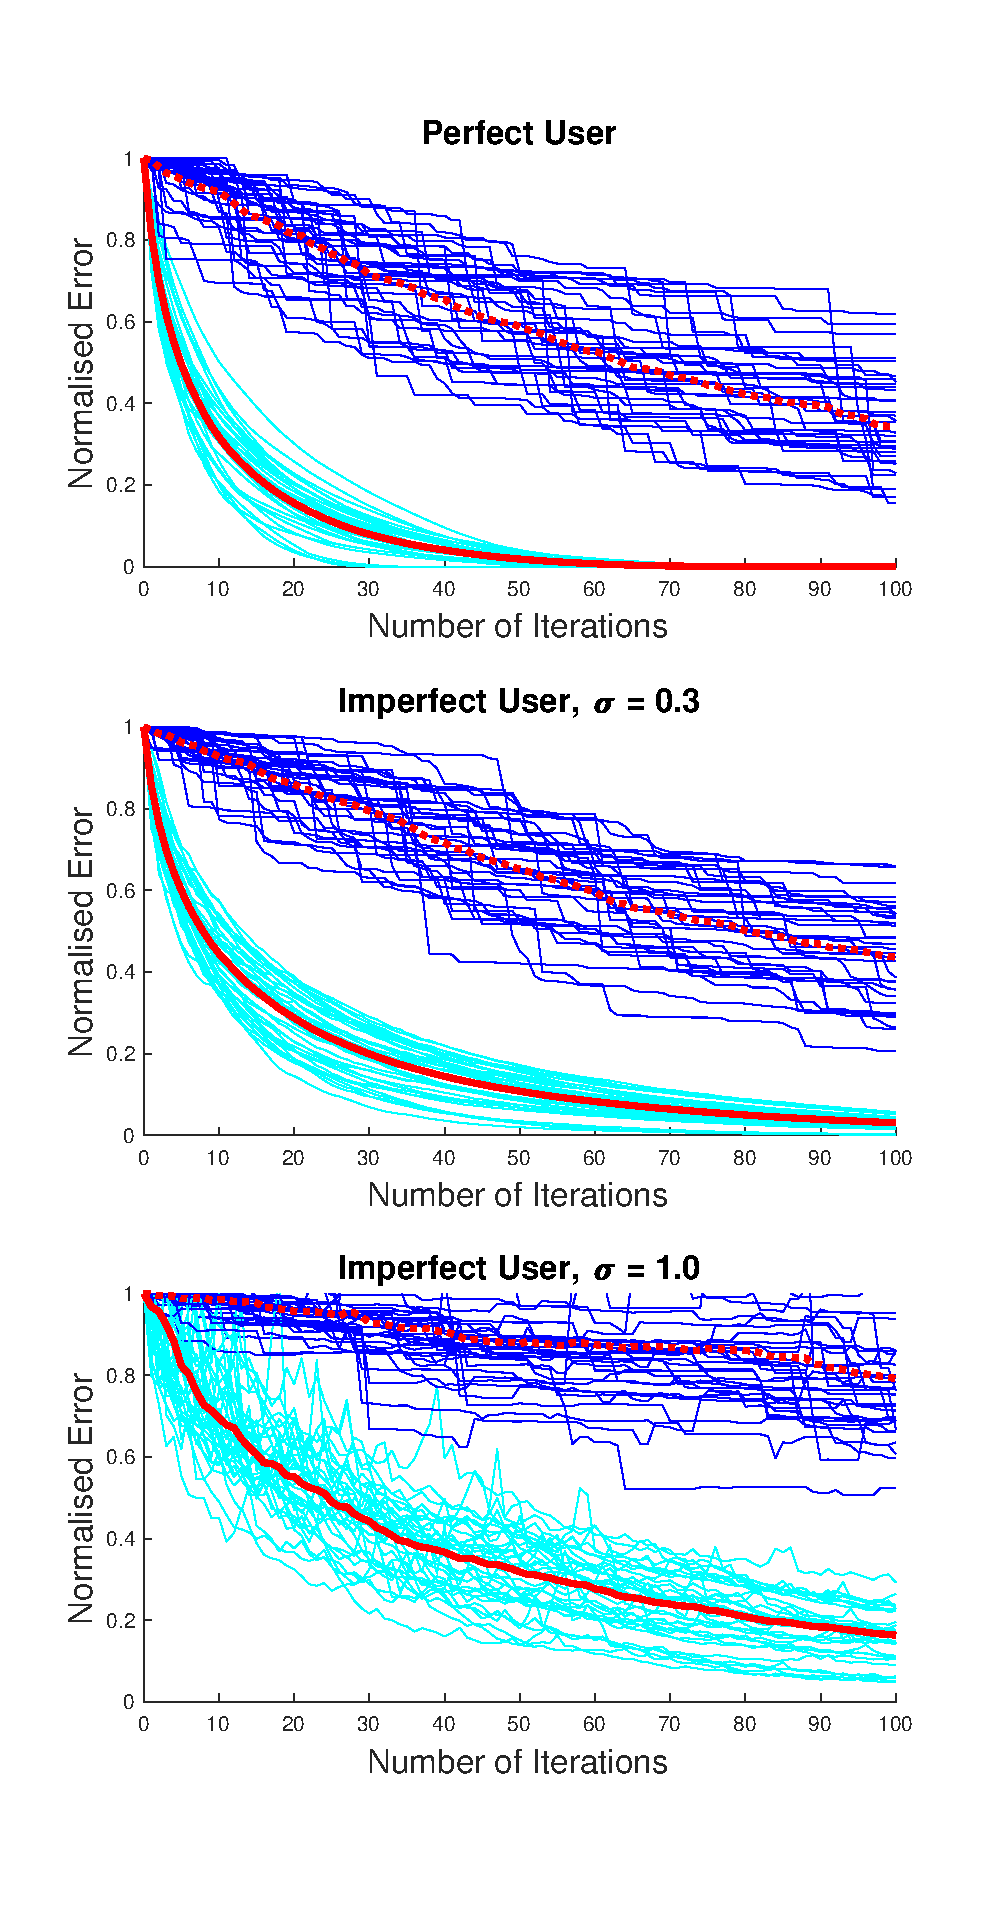
\includegraphics[trim  ={0, 2.3cm, 0, 1.5cm}, clip, width = 3.1in]{TradInterfaceTests1.eps}
	\caption{Perfect/Imperfect user tests for Traditional Interface}
	\label{fig:TradTest1}
	
%	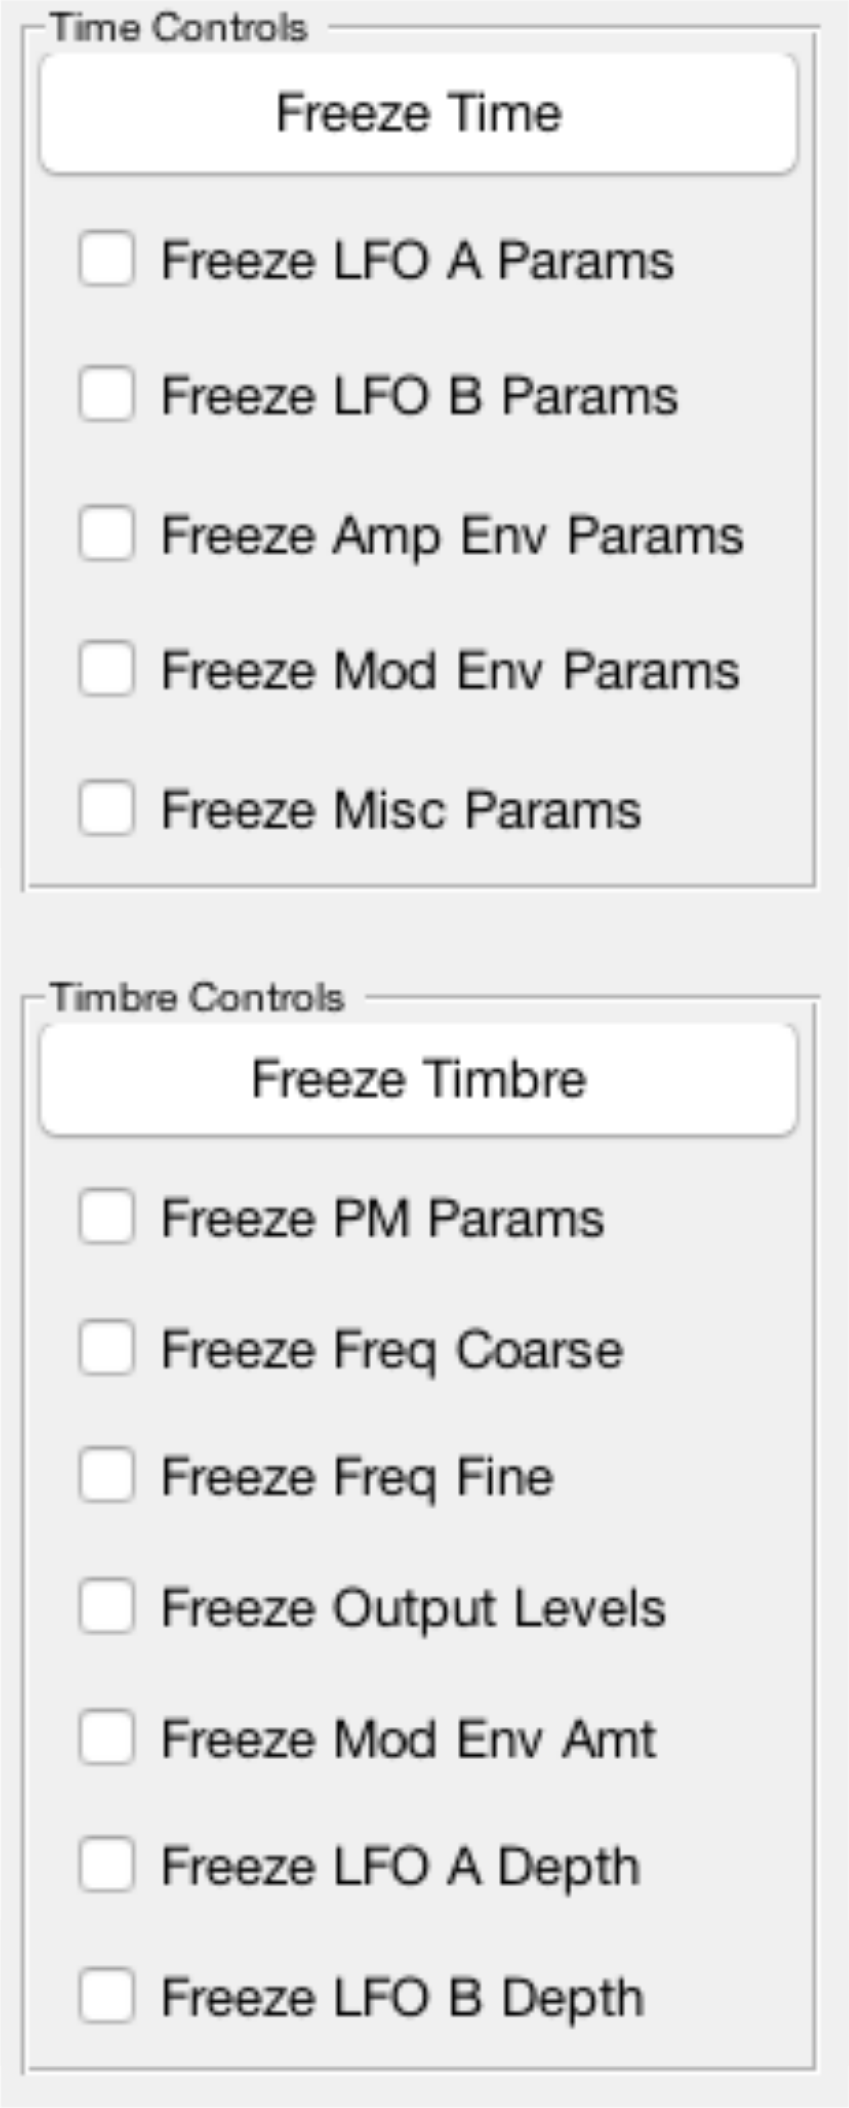
\includegraphics[width = \textwidth/3]{FreezeParams2.png}
%	\caption{Parameter Freezing}
%	\label{fig:FreezeParams}
	
	\vspace{-60pt}
	
\end{wrapfigure}
Perfect/Imperfect user tests were carrried out on the Blending Interface, using each of the 36 presets as a goal preset, and starting from the closest preset to the goal preset. The results of these tests are shown in Fig. \ref{fig:TradTest1}. The cyan lines are individual instances of the Perfect Order test. The blue lines are individual instances of the Random Order test. The solid red lines are the mean of the Perfect Order tests (solid), and the Random Order tests (dotted). 

For low values of $\sigma$, the Perfect Order tests folllows a smooth, approximately exponentially decreasing, curve. For high values of $\sigma$, and when the Random Order is used, the error decreases in a much less smooth manner. In all cases the Perfect Order gives a substantially faster convergence time. A comparison of the mean error for various values of $\sigma$ is shown in Fig. \ref{fig:TradTest2}. These results suggest that \textbf{the main limitation when using a Traditional Interface is not the accuracy with which the parameters are set, but the choice of parameter}.
\begin{figure}
	\centering
%	\vspace{-40pt}
	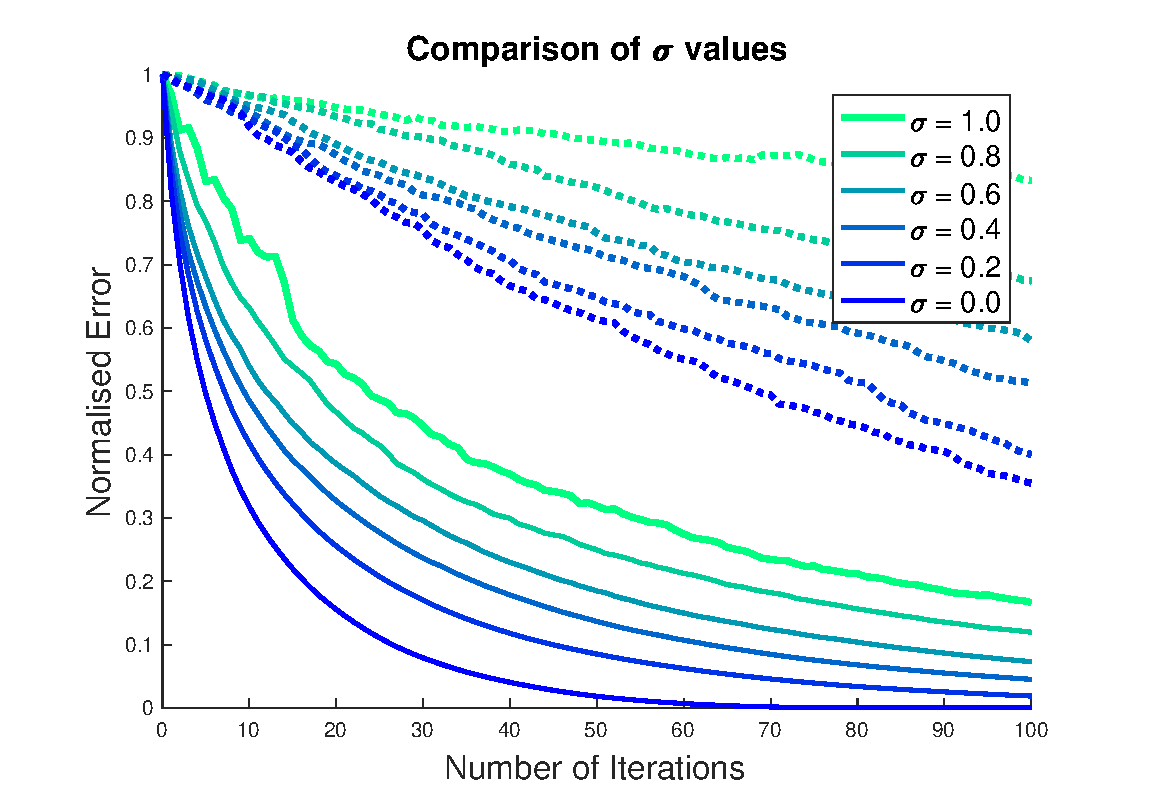
\includegraphics[width = 5in]{TradInterfaceTests2.eps}
	\caption{Perfect/Imperfect user tests for Traditional Interface. Perfect Order shown with solid lines, Random Order shown with dotted lines. The Parameter order has a much more significant effect than the Imperfectness of the user.}
	\label{fig:TradTest2}
%	\vspace{-30pt}
	
\end{figure}

\subsection{Selection Interface}\label{sec:SelectionEval}
A similar evaluation was carried out with the selection interface. Again all 36 presets were used as goal presets, with the closest preset used each time as the starting point. For each test, the PCA values were calculated for the remaining 35 presets, simulating the situation where the PCA Macros were being used to find a brand new preset. As before, two parameter orders were tested: the Macro Controls were visited cyclically in order of PCA number, or visited in a random order. For each iteration of the test, the MATLAB 'Patternsearch' search algorithm was used to minimise the cost function for a particular Macro Control. (WHY WAS THIS USED?)\\ 
A key question with the interface is whether the 'Global' or 'Time/Timbre' version of the PCA Macro Controls should be used. The results for a test with the combination of both sets of macros is shown in Fig. \ref{fig:PCAtest1}, and a comparison of the mean results for the different macro configurations is shown in Fig. \ref{fig:PCAtest2}.
\begin{figure}

\hspace{-60pt}
	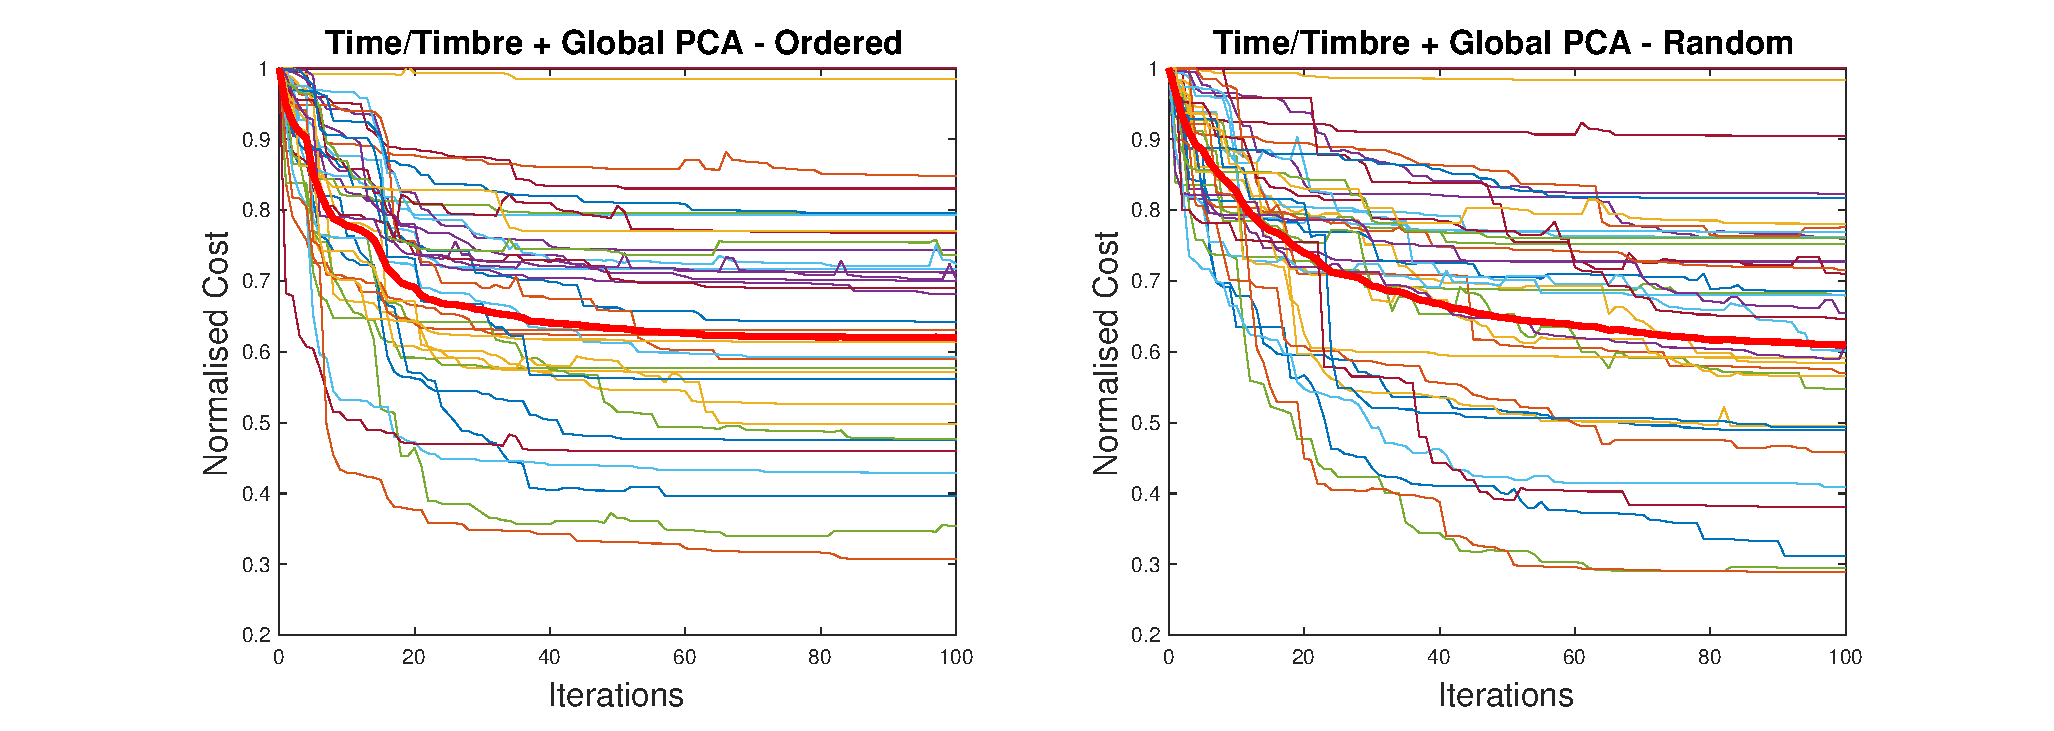
\includegraphics[width = 8in]{PCAInterfaceTests1.eps}
	\caption{Ordered/Random user tests for Selection Interface}
	\label{fig:PCAtest1}
	%	\vspace{-30pt}
\end{figure}
\begin{figure}
	\centering
		\vspace{-40pt}
	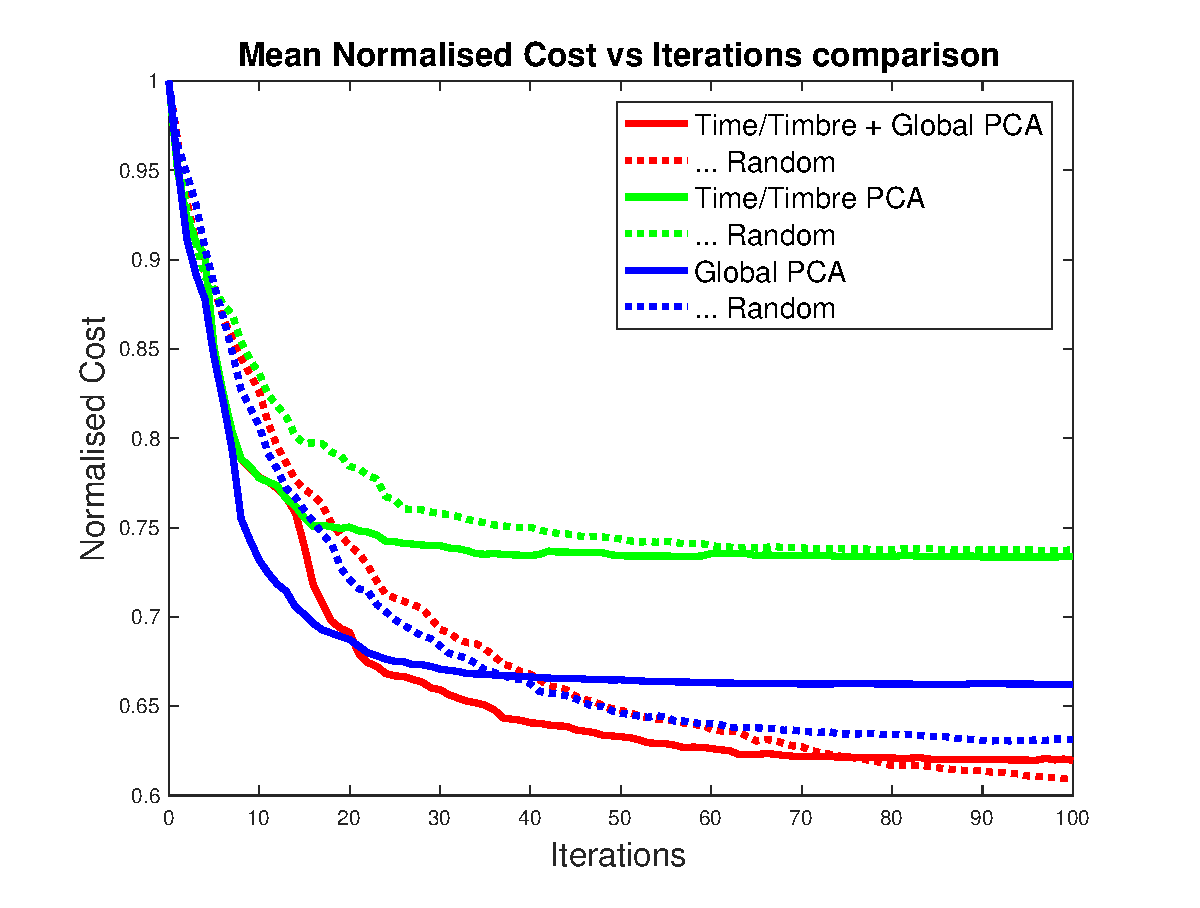
\includegraphics[width = \textwidth]{PCAInterfaceTests2.eps}
	\caption{Comparison of Macro Types - All of the Macro Controls have a similar initial rate of cost reduction, but the Global Macro Controls have a better steady state value than the Time/Timbre Macro Controls.}
	\label{fig:PCAtest2}
	%	\vspace{-30pt}
\end{figure}
%MAYBE NEED TO DO THE IMPRERFECT USER TESTS ON THE MACRO CONTROLS.

Some points to note from these results:

As shown in Fig. \ref{fig:PCAtest1}, for different preset goals, the effectiveness of the PCA Controls varies significantly. In the best case the error drops very rapidly, falling 50\% in the first 10 iterations. In the worst case the error doesn't decrease at all. This suggests that, for this particlar task at least, having the same Macro Controls for each preset may not be ideal, and so a new approach which in some way optimises the Macro Controls per preset would be worth pursuing. However this comes at the cost of the user being less familiar with what the Macro Controls are actually doing (\S \ref{sec:GlobalTimeTimbre}).

In all cases the mean error converges to a non-zero steady state value. This is due to the limited degrees of freedom when using the Macro Controls. This means that the Macro Controls alone cannot be used to perfectly match a goal preset.

When the Global Macro Controls are being used, after a large number of iterations, the random order manages to decrease the error past the cyclic order. It is likely that this is due to the cyclic order getting stuck in a local optimum due to the naive 'one parameter at a time' (BETTER NAME FOR THIS) search algorithm.

Finally, each of the combinations of controls has a similar initial rate of error reduction, but the 'Global' Macro Controls appear to have a significant advantage over the 'Time/Timbre' Macro Controls over larger numbers of iterations. This is likely due to the fact that the Global Macro Controls have access to principal components 1 to 8, whereas the 'Time/Timbre' Macro Controls on have access to two sets of principal components 1 to 4. The combination of both sets of Macro Controls gives the lowest mean error overall, which is unsurprising as it has the most degrees of freedom, and it has a comparable error reduction rate as the 'Global' Controls.

Based on this it is concluded that it is worth keeping both sets of macro controls for the user to be able to select between, especially as the Time/Timbre Macro Controls may lead to more semantically meaningful controls due to the seperation of Time and Timbre. (JUSTIFY THIS MORE)

\subsection{Blending Interface} \label{sec:BlendingEval}
The Blending interface was evaluated in a similar manner. For each of the 36 possible goal presets, the closest three presets to it were found, and these used as preset A, B and C in the blending algorithm. MATLAB's Patternsearch was again used in each iteration to optimise the position of the mouse in the Blending Interface to minimise the parameter based error metric. 

Results of this test are shown in Figure \ref{fig:BlendingTest1}
\begin{figure}
	%\centering
	\hspace{-70pt}
	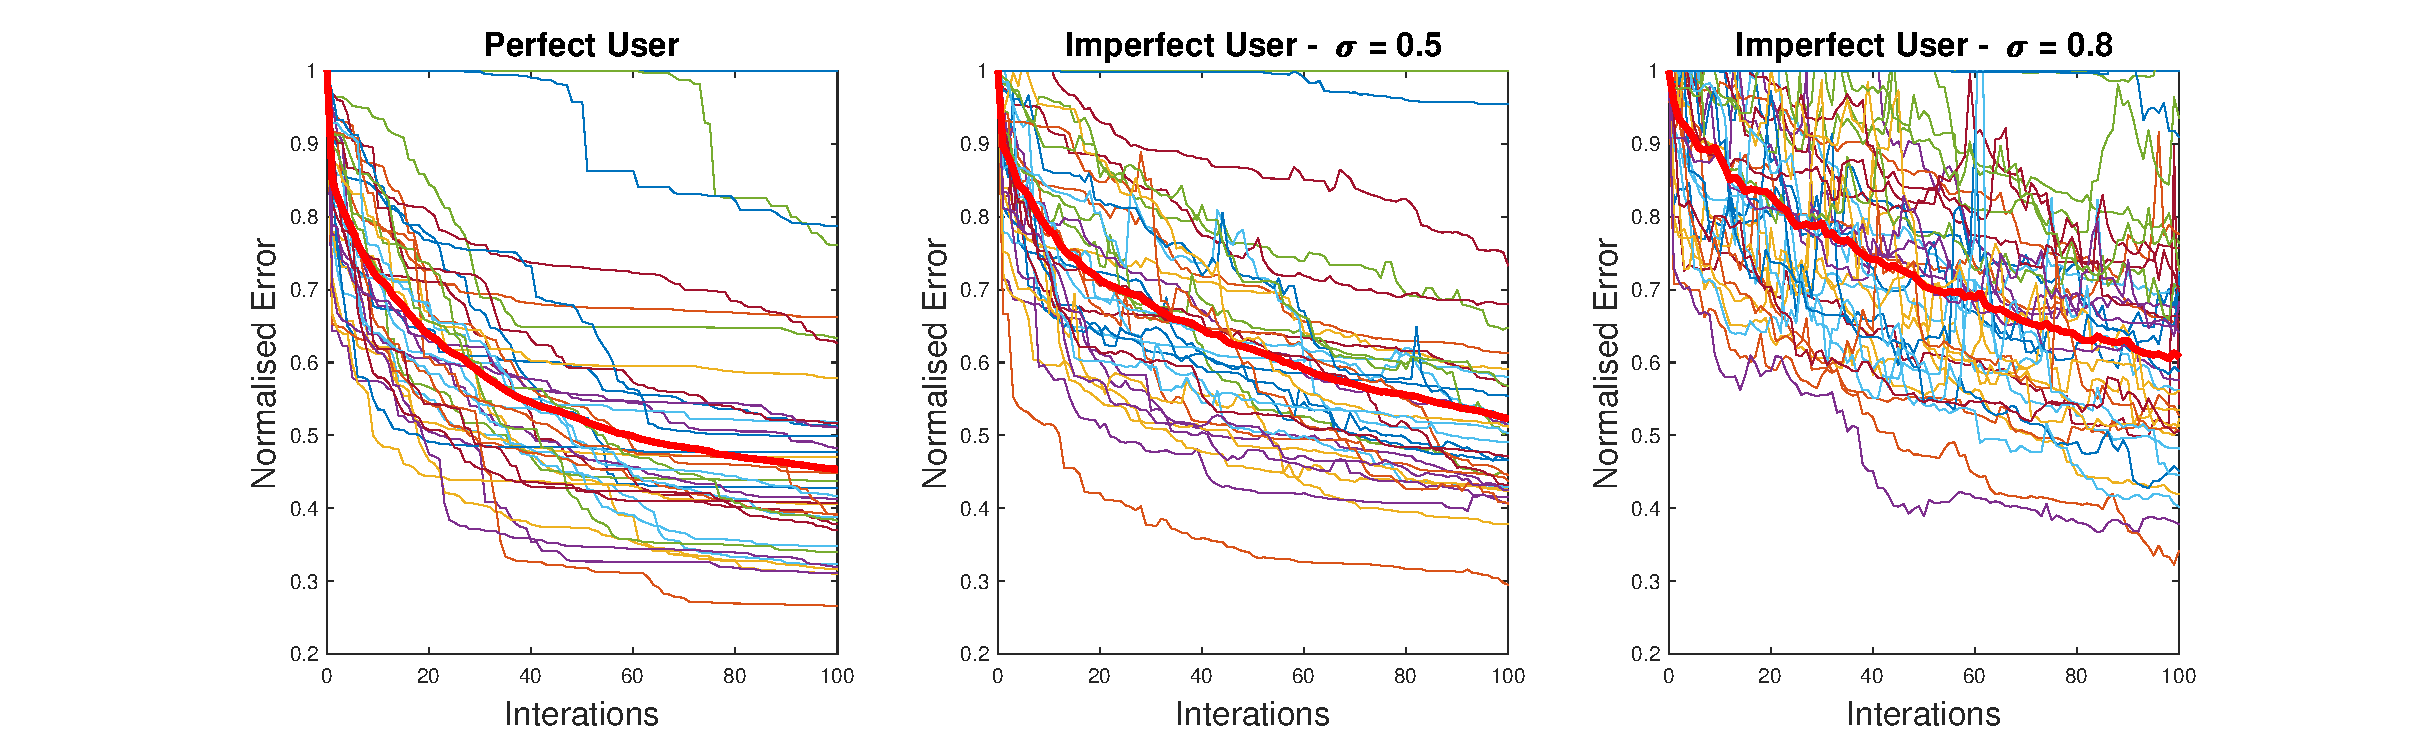
\includegraphics[width = 8in]{BlendingInterfaceTests1.eps}
	\caption{Perfect/Imperfect User tests for Blending Interface}
	\label{fig:BlendingTest1}
	%	\vspace{-30pt}
\end{figure}
On average, there is n rapid decrease in error during the first iteration, followed by an approximately expenential decrease in error.
As in the Selection Interface, there are some tests in which the error barely decreases at all, and some in which the error decreases very quickly, however the variance of the different tests is less than in the PCA interface. For the Perfect User, error is monotoically decreasing, but this is not always the case for the imperfect user, and for real users of the system(EVIDENCE?). This reinforces the need for the Selection History Plot (See Section \ref{sec:BlendingDescription}), which allows users to select several of the local minima in the error plot to resume blending with. (MAYBE MORE DETAIL)

\section{Comparison of Interfaces}
A comparison of the test results from all three interfaces is shown in Figure \ref{fig:CombinedTest1}.  COULD DO A TABLE OF INITIAL RATE OF ERROR REDUCTION
\\
The fastest converging test is the Perfect User with Perfect Order on the Traditional Interface, and the slowest converging test is the Imperfect User with Random Order on the Tradtional interface. Interestingly, the order at which the parameters are visited has a much more significant affect than the perfectness of the user. This is due to the Imperfect user model having a zero mean error, so after visiting a parameter several times, the value will converge to the correct value. This result demonstrates that the Traditional Interface can simultaneously be the best possible, and worst possible interface to control a synth with, depending on the experience level of the user, and the intuitiveness of the parameters.

The initial error reduction rate of the Blending Interface is very fast, comparable with the Perfect User of the Traditional interface. The main reason for the initial speed of the Blending Interface is that in the first iteration, it blends between 3 presets, all close to the goal preset, allowing the first iteration to be a lot less random than subsequent steps. (EXPLAIN BETTER)\\
A key advantage of the Blending Interface is that it removes the need for the user to choose which order to alter the parameters which, as previously described, is the main factor in speed of the Traditional Interface. (MORE DETAIL?)\\
 Over a larger number of iterations, Blending Interface is supassed by the Traditinonal interface with random order. This suggests that the preset generation algoithm is not optimal, as after a while it becomes faster to just sequentially offer the user a random parameter. However, as the user has the option to freeze parameters, and the option to switch to the other interfaces at any point, this may not be an issue. \\
Before converging to their steady state value, the macro controls have quite a fast rate of error reduction - halfway betwen the Perfect User with Perfect or Random Order. This can be partially explained as the Macro Contols allow all of the synthesiser parameters to be varied at once. This also suggests that, as the PCA was carried out on a set of presets, it is likely that the principal components are pointed in a more useful direction than if they'd been selected randomly. (WRITE BETTER)\\
These results suggest that a good workflow for editing synthesis parameters is as follows:
\vspace{-3em}
\begin{itemize}
	\setlength\itemsep{-1.2em}
	\item Find closest 3 presets to desired sound
	\item Use Macro Controls to refine these presets further ($\approx$ 5 iterations per preset)
	\item Use Blending Interface to combine these presets together and further refine ($\approx$ 10 iterations)
	\item Use Traditional interface for final refining of preset. ($\approx$ 20 iterations)
\end{itemize}
\vspace{-0.5em}
The full Interface allows such a process to be carried out, and allows the user to swicth back and forth between the interfaces as often as necessary.

As these tests have only been carried out on one set of presets for one particular synthesiser, an important follow-up work to this project is to validate these results on other synthesisers. As these tests are purely parameter based, the tests could potentially be carried out before doing a full integration of the interface with other synthesisers, as only the set of presets for each synth are needed.

\begin{figure}
	\hspace{-50pt}
	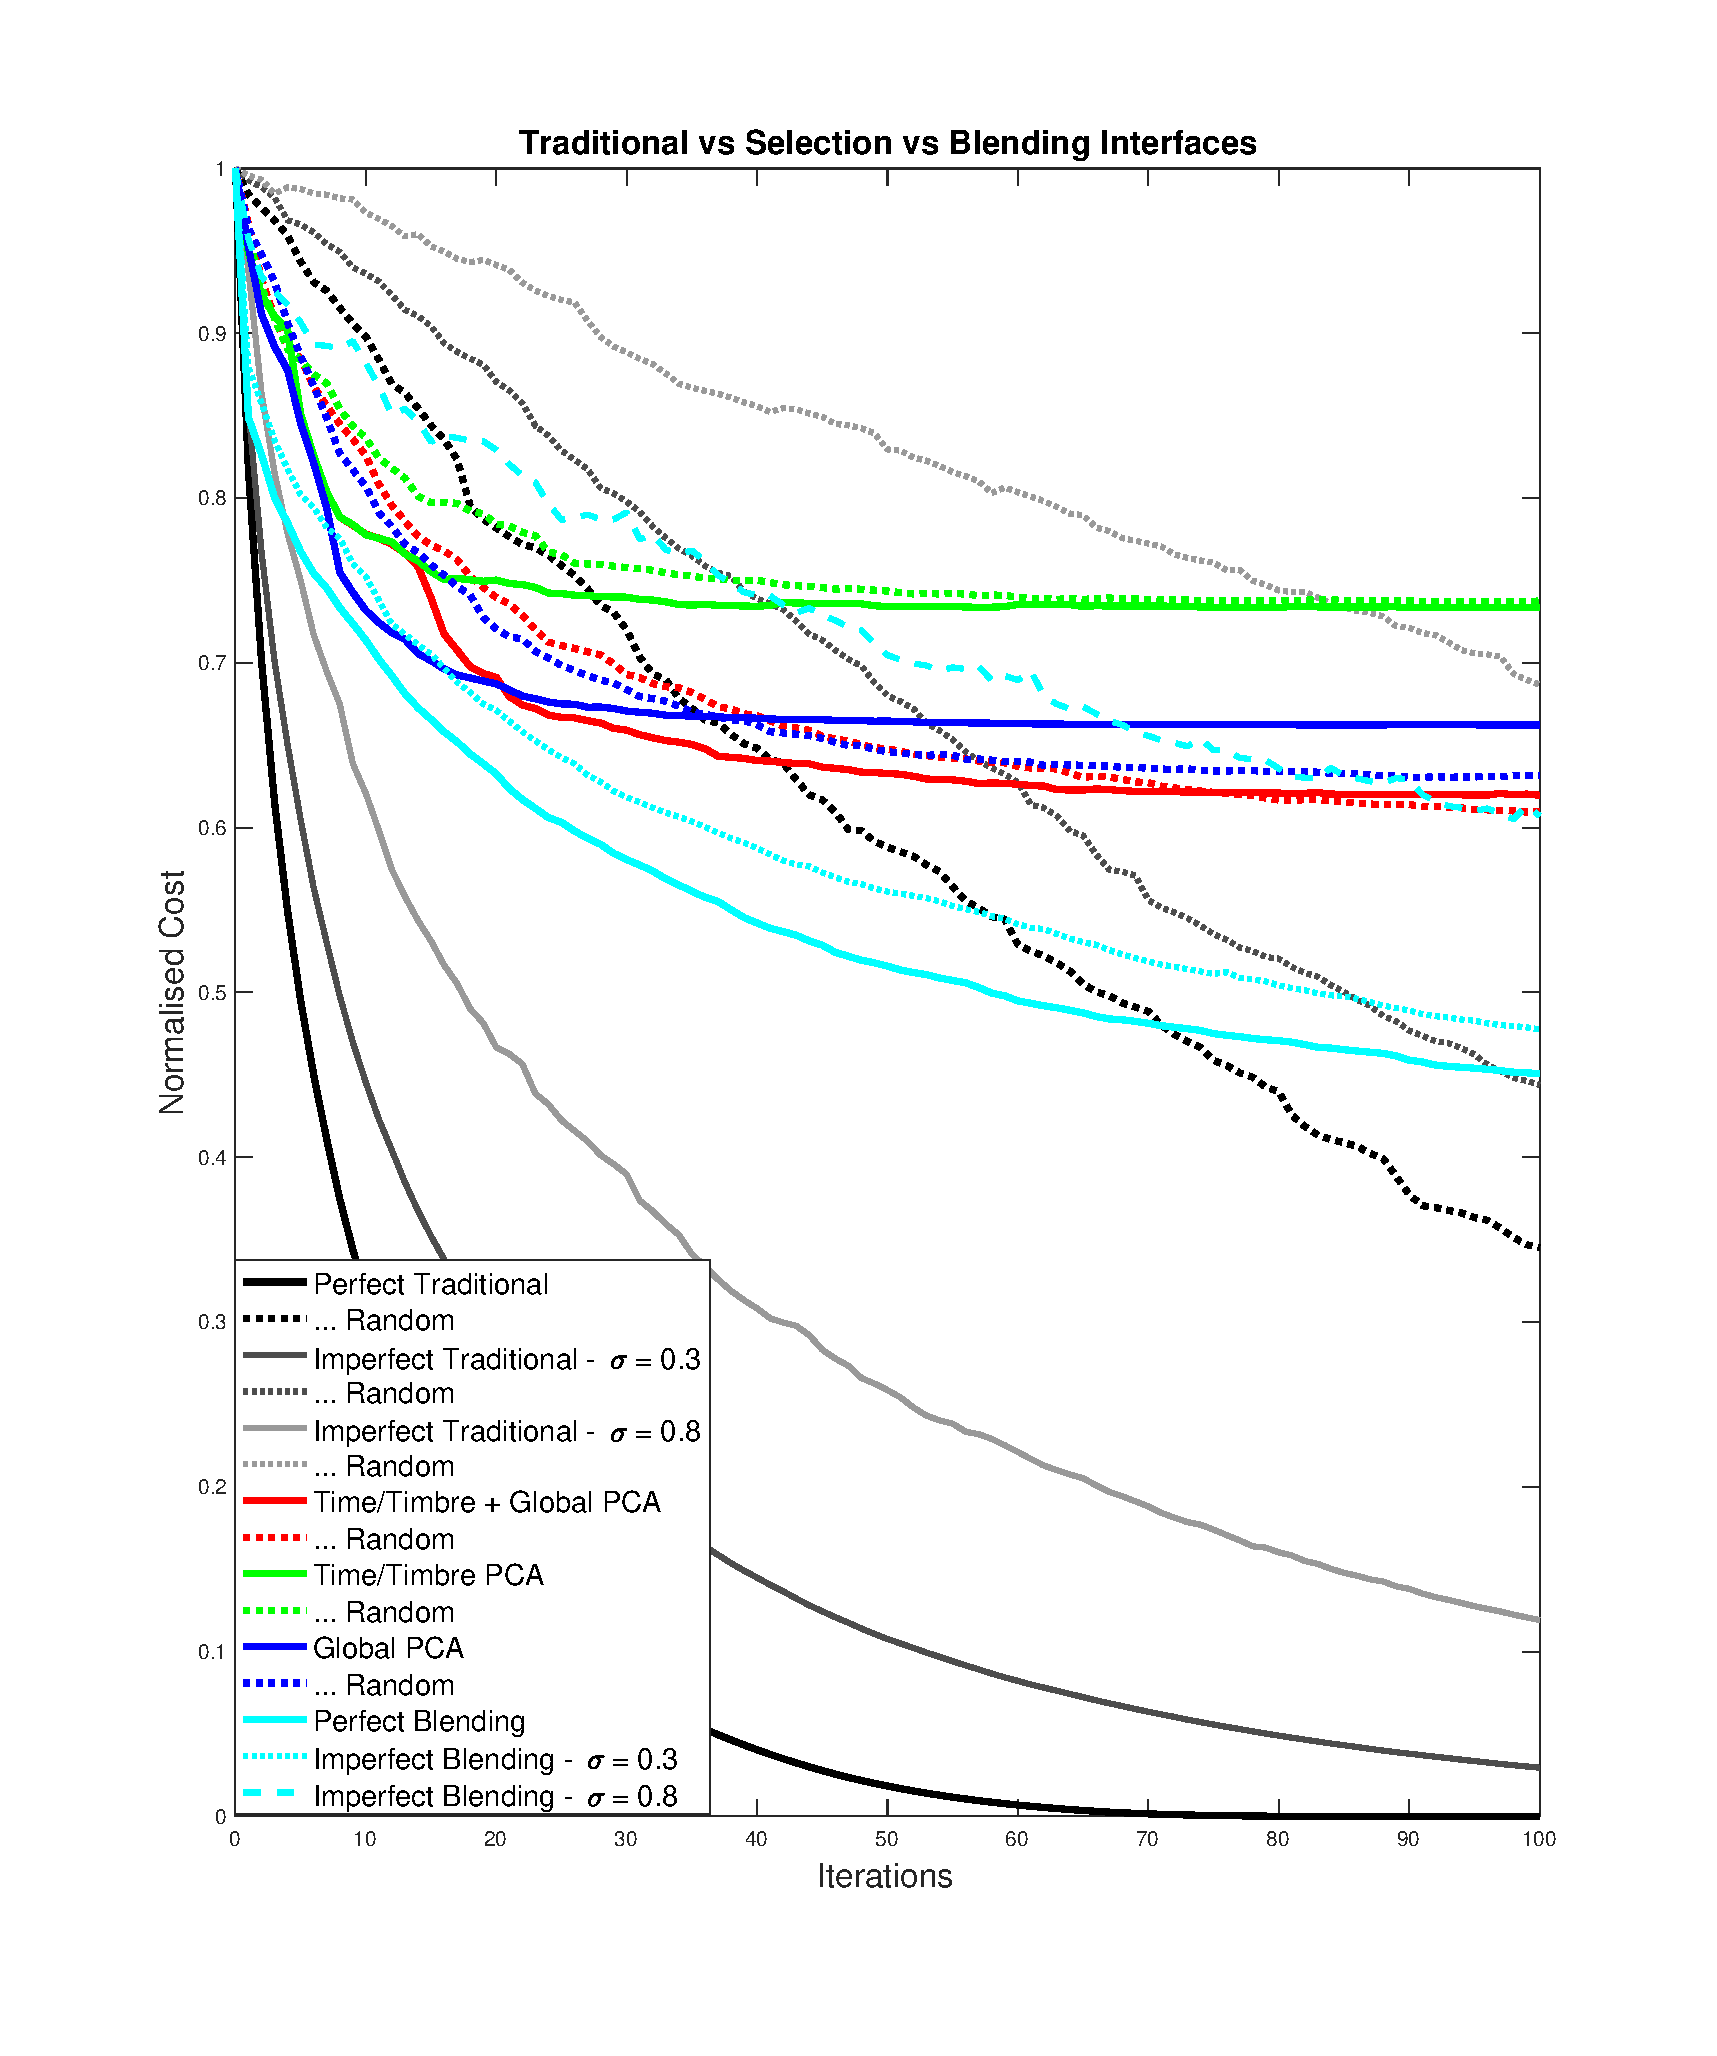
\includegraphics[trim = {0, 2cm, 0, 0}, clip, width = 7.6in]{comparisonOfAllInterfaceGraph3.eps}
	\caption{Comparison of Interfaces - The Blending Interface, and Selection Interface both have initial rates of error reduction faster than the traditional interface with random order (WRITE MORE DESCRIPTION HERE)}
	\label{fig:CombinedTest1}
	%	\vspace{-30pt}
\end{figure}

\section{EARS-model based evaluation of interface}\label{sec:EARS}
In Table \ref{tab:EARStable}, the three interfaces are evaluated in terms of the EARS model from Section \ref{sec:Tubb} \cite{TubbThesis}.
A conclusion which can be drawn is that the interfaces enables Exploratory, Algorithmic, and Reflective process well, but is not suited to skilled interactions. One of the interfaces could be redisigned with this in mind, or a fourth interface could be introduced.  It should be designed for use with multidimensional controllers, and involve moving through a parameter space consisting solely of the nice sounds of the synthesiser. An Interactive Machine Learning system such as the \emph{Wekinator} \cite{Wekinator} would be well suited to this task, however more work needs to be done to integrate this approach with the other 3 interfaces.
\begin{table}[h]
	\hspace{-1cm}
	\begin{tabular}{|l|l|l|l|l|L|}
		\hline
		\rowcolor[HTML]{EFEFEF} 
		Interface                           & Exploratory & Algorithmic & Reflective & Skilled & Comments                                                                                                                                                                                                                                                                                                                                                                       \\ \hline
		\cellcolor[HTML]{EFEFEF}Traditional & Maybe        & Yes          & No          & No       & Can be used for exploratory and algorithmic depending on the skill level of the user                                                                                                                                                                                                                                                                \\ \hline
		\cellcolor[HTML]{EFEFEF}Selection   & Yes          & No           & Yes         & No       & \begin{tabular}[c]{@{}L@{}}Exploration by browsing and varying presets. \\ Reflective as easy comparison of presets with combined and varied presets.\end{tabular}                                                                                                                                                                                                            \\ \hline
		\cellcolor[HTML]{EFEFEF}Blending    & Yes          & Maybe        & Yes         & Maybe    & \begin{tabular}[c]{@{}L@{}}Well suited to exploratory, due to simple interface and preset generation. \\ May be used algorithmically due to parameter freezing.\\ The Selection History graph enables reflective comparison and combination.\\ May be used as a skilled strategy, but is not optimised for this approach. Too low dimensional and unpredictable.\end{tabular} \\ \hline
	\end{tabular}
\caption{EARS Model evaluation of synthesiser interfaces}
\label{tab:EARStable}
\end{table}



%\chapter{User tests and Interviews}
%A rigourous user study would require time and resourses that this project is incapable of, however the interface has been shown to a number of musicians, and some feedback shown below:
%
%NEED TO DO THESE INTERVIEWS
%...

\chapter{Conclusion}
The interface proposed in this project has many benefits over a traditional synthinterface, as has been designed following design heuristics from the fields of Human Computer Interaction and Creative Cognition. Based on simulated user studies, the interface has at least as good performance as a traditional interface when carrying out search based tasks, and based on real user feedback it has many advantages in terms of creativity (If don't have interviews CANT INCLUDE). \\
Synth preset datasets are not random, and information can definitely be learned from them. PCA combined with Histogram Equalisation has been identified as a useful dimensionality reduction tool for synthesiser parameters, and several preset generation algorithms have been developed and tested. \\
The interface has also been tested in a different domain, Image Filtering, with promising results. It could easily be applied to many other use cases, such as stage lighting design, or parametric 3D design, as each has a high dimensional parameter set which can be readily controlled over interfaces such as OSC.
\section{Further Work}
The evaluation of this interface was only carried out on a single synth, due to the project's time constraints. An immediate goal is to validate the conclusions from this work on several other synths. The next synths to test should be from other categories, such as \emph{subtractive}, \emph{additive} and \emph{physical modelling} syntheses. It is non-trivial to extend this work to modular synths, as there is neither a fixed number of parameters, nor a fixed achitecture, so different presets may be uncomparable with any common error metric.

The interface has been designed to be as general purpose as possible, allowing it to control arbitrary synths over the OSC protocol, but due to a lack of standardisation between soft synths, and lack of implementation time, more work needs to be done to create a truly general purpose soft-synth controller. As many soft-synths are in the \emph{Virtual Studio Technology (VST)} format, making a version of the interface with acts as a \emph{VST host}, and uses the parameter retrieval and preset storage functionality of VSTs is a good next goal if this project is continued.

The interface has been designed with touch-screen contollers in mind, so it would be interesting to implement the interface on a touch screen. Either a dedicated app could be made, or the customisable OSC controllers \emph{Lemur} or \emph{Mira} could be used. The interface could be further extended by taking into consideration the \emph{multi-touch} capabilities of modern touchscreens.

When the Blending Interface is used, the user carries out a large number of interactions, all of which show a users preference over hyperplanes of parameter settings. If recorded, it may be possible to use these interactions to form a training set for more sophisticated preset generation algorithms, using techniques such as bayseian optimisation which require large ammount of training data when used in high dimensional problems \cite{PreferenceGallery}. As each interaction finds the optimum in a hyperplane, the interactions have the potentially to be more information dense than binary choices.

Aside from the initial confiuration of presets A, B and C, the Blending Interface currently does not use the preset dataset in its preset generation algorithm. Due to the effectiveness of using this dataset in the Selection Interface, the inclusion of this data is a worthwhile area of further research.

In typical synths, the parameters have a hierarchical nature, as the synthesis algorithm is usally made up of several modules, each with their own parameters and/or sub modules. Many synths store their presets in the \emph{Javascript Object Notation (JSON)} format, and use such hierarchies to make clean data structures. It may be possible to make use of this hierarchical parameter structure to deduce covariances between parameters, as those in the same module are likely to be much more co-dependant than those in seperate modules. This could be used to refine the preset generation and comparison algorithms, and help to detect and correct cases of permutation ambiguity. However this approach has several challenges, most importantly there is a lack of standardisation of preset storage hierarchies.

%The Native Kontrol Standard, is a standardard

\begin{thebibliography}{9}
\singlespacing

\bibitem{Wavetable}
Ableton.com. (2018). \emph{Wavetable | Ableton}. [online] Available at: \url{https://www.ableton.com/en/packs/wavetable/} [Accessed 18 Apr. 2018].

\bibitem{AppleSynth}
Documentation.apple.com. (2009). \emph{A Brief History of the Synthesiser}. [online] Available at: \url{https://documentation.apple.com/en/logicstudio/instruments/index.html#chapter=A\%26section=5\%26tasks=true} [Accessed 20 Apr. 2018].

\bibitem{PreferenceGallery}
Brochu, E. et al. 2010. \emph{A Bayesian interactive optimization approach to procedural animation design}. Proceedings of the 2010 ACM SIGGRAPH/Eurographics Symposium on Computer Animation (SCA '10). Eurographics Association, Goslar, Germany, 103-112.

\bibitem{FM}
Chowming, J.M. (1977). \emph{The Synthesis of Complex Audio Spectra by Means of Frequency Modulation}.

\bibitem{Voronoi}
Dobrin, A. (2005). \emph{A review of properties and variations of Voronoi diagrams}. 

%\bibitem{SY22}
%Encyclotronic. (2018). \emph{Yamaha SY22 Vector Synthesizer}. [online] Available at: \url{https://encyclotronic.com/synthesizers/yamaha/sy22-r345/} [Accessed 18 Apr. 2018].

\bibitem{InfiniteDrum}
Experiments.withgoogle.com. (2017). \emph{The Infinite Drum Machine by Manny Tan \& Kyle McDonald} - AI Experiments. [online] Available at: \url{https://experiments.withgoogle.com/ai/drum-machine} [Accessed 18 Apr. 2018].

\bibitem{Wekinator}
Fiebrink, R. et al. (2010). \emph{The Wekinator: A System for Real-time, Interactive Machine Learning in Music}. Proceedings of The Eleventh International Society for Music Information Retrieval Conference (ISMIR 2010). 

\bibitem{ICMC}
Hantrakul, L. and Kaczmarek, K. (2014). \emph{Implementations of the Leap Motion in sound synthesis, effects modulation and assistive performance tools}. In: International Computer Music Conference. 

\bibitem{RatingRanking}
Harzing, A et al. 2009. \emph{Rating versus ranking: What is the best way to reduce response and language bias in cross-national research?}.
International Business Review,
ISSN 0969-5931

\bibitem{MappingStrategies}
Hunt, A. \& Kirk, R. 2000. \emph{Mapping Strategies for Musical Performance}. Trends in Gestural Control of Music

\bibitem{EvolutionaryInteractive}
J\'{o}nsson B et al. 2015. \emph{Interactively Evolving Compositional Sound Synthesis Networks}. In Proceedings of the 2015 Annual Conference on Genetic and Evolutionary Computation (GECCO '15), New York. DOI: \url{http://dx.doi.org/10.1145/2739480.2754796}

\bibitem{UGen}
Kersten, S. \emph{skUG SuperCollider UGen library}, 2008. \url{http://space.k- hornz.de/software/skug/}.

\bibitem{LinnKeynote}
Linn, R. \emph{Keynote}.  Audio Developer Conference, 2016. \url{https://www.youtube.com/watch?v=3bHGeSv37rU} [at 19:00]

\bibitem{Interpolation}
Marier, M. (2012). \emph{Designing Mappings for Musical Interfaces Using Preset Interpolation}. NIME.

\bibitem{NonOrthogonal}
Miguel (https://math.stackexchange.com/users/95625/miguel), \emph{Equation for non-orthogonal projection of a point onto two vectors representing the isometric axis?}, (version: 2017-03-07): \url{https://math.stackexchange.com/q/1123586}

\bibitem{Massive}
Native-instruments.com. (2007). \emph{MASSIVE}. [online] Available at: \url{https://www.native-instruments.com/en/products/komplete/synths/massive/} [Accessed 18 Apr. 2018].

\bibitem{SynthTypes}
Nicol, C. (2005). \emph{Development and Exploration of a Timbre Space Representation of Audio}. Ph.D. University of Glasgow.
References

\bibitem{OSC}
Opensoundcontrol.org. (2002). \emph{Introduction to OSC} [online] Available at: \url{http://opensoundcontrol.org/introduction-osc} [Accessed 18 Apr. 2018].

\bibitem{IphoneProducer}
Pierce, D. (2017). \emph{The hot new hip-hop producer who does everything on his iPhone}. [online] WIRED. Available at: \url{https://www.wired.com/2017/04/steve-lacy-iphone-producer/} [Accessed 20 Apr. 2018].

\bibitem{GenSynth}
Rice, David. (2015). \emph{GenSynth: Collaboratively Evolving Novel Synthetic Musical Instruments}. 10.13140/RG.2.1.4691.6001. 

\bibitem{ActiveLearning}
Settles, Burr. (2010). \emph{Active Learning Literature Survey}. University of Wisconsin, Madison.

\bibitem{PCA}
Shlens, D. (2014). \emph{A Tutorial on Principal Component Analysis}. arXiv:1404.1100 [cs.LG]

%\bibitem{SoftTube}
%Softube.com. (2016). Softube - Modular. [online] Available at: \url{https://www.softube.com/modular} [Accessed 18 Apr. 2018].

\bibitem{EvolvedAudioEffects}
Smith, B.D. (2017) \emph{Play it Again: Evolved Audio Effects and Synthesizer Programming}. In: Computational Intelligence in Music, Sound, Art and Design. EvoMUSART 2017. Lecture Notes in Computer Science, vol 10198. Springer, Cham.

\bibitem{TubbThesis}
Tubb, R. (2016). \emph{Creativity, Exploration and Control in Musical Parameter Spaces}. Ph.D. Queen Mary University of London.

\bibitem{Synth}
Vail, M. (2014). \emph{The Synthesizer}. New York, NY: Oxford University Press.

\bibitem{FS1R}
Vintagesynth.com. (2012). \emph{Yamaha FS1R | Vintage Synth Explorer}. [online] Available at: \url{http://www.vintagesynth.com/yamaha/fs1r.php} [Accessed 18 Apr. 2018].

\bibitem{BayesOptDimensionality}
Wang, Z. et al. 2016. \emph{Bayesian Optimization in a Billion Dimensions via Random Embeddings}. arXiv:1301.1942 [stat.ML]

\bibitem{YeeKing}
Yee-King, M. (2011). \emph{Automatic Sound Synthesizer Programming: Techniques and Applications}. Ph.D. University of Sussex.

\bibitem{GenComparison}
Yee-King, M J. 2016. \emph{The Use of Interactive Genetic Algorithms in Sound Design: A Comparison Study}. Computers in Entertainmnent, 14(3), [Article]

\bibitem{NSynth} \emph{Neural Audio Synthesis of Musical Notes with WaveNet Autoencoders}. Engel, J., Resnick, C., Roberts, A., et al.\ 2017, arXiv:1704.01279 

\bibitem{HistogramEqualisation}
Singh, P. et al. (2015). \emph{Histogram Equalization: A Strong Technique for Image Enhancement}. International Journal of Signal Processing, Image Processing and Pattern Recognition. %8. 345-352. 10.14257/ijsip.2015.8.8.35. 

\bibitem{ExplorationExploitation}
Besbes, O. et al. 2014.\emph{Optimal Exploration-Exploitation in a Multi-Armed-Bandit Problem with Non-stationary Rewards}.	arXiv:1405.3316

\end{thebibliography}
\end{document}  